%%%%%%%%%%%%%%%%%%%%%%%%%%%%%%%%%%%%%%%%%%%%%%
% The Python Digraph module doc version 1..0
% R.Bisdorff March 2006
% Current revision $Revision: 1.18 $
%%%%%%%%%%%%%%%%%%%%%%%%%%%%%%%%%%%%%%%%%%%%%%
\documentclass{article}
\usepackage{hyperlatex}
\usepackage{xspace}
\usepackage{verbatim}
%% Comment out the following line if you do not have Babel
\usepackage[english]{babel}
\W\usepackage{longtable}
\W\usepackage{makeidx}
\W\usepackage{frames}
\T\usepackage{graphicx}
% \W\usepackage{hyperxml}

%\newcommand{\new}{\htmlimg{new.png}{NEW}}

\newcommand{\printindex}{%
  \htmlonly{\HlxSection{-5}{}*{\indexname}\label{hlxindex}}%
  \texorhtml{%%%%%%%%%%%%%%%%%%%%%%%%%%%%%%%%%%%%%%%%%%%%%%
% The Python Digraph module doc version 1..0
% R.Bisdorff March 2006
% Current revision $Revision: 1.18 $
%%%%%%%%%%%%%%%%%%%%%%%%%%%%%%%%%%%%%%%%%%%%%%
\documentclass{article}
\usepackage{hyperlatex}
\usepackage{xspace}
\usepackage{verbatim}
%% Comment out the following line if you do not have Babel
\usepackage[english]{babel}
\W\usepackage{longtable}
\W\usepackage{makeidx}
\W\usepackage{frames}
\T\usepackage{graphicx}
% \W\usepackage{hyperxml}

%\newcommand{\new}{\htmlimg{new.png}{NEW}}

\newcommand{\printindex}{%
  \htmlonly{\HlxSection{-5}{}*{\indexname}\label{hlxindex}}%
  \texorhtml{%%%%%%%%%%%%%%%%%%%%%%%%%%%%%%%%%%%%%%%%%%%%%%
% The Python Digraph module doc version 1..0
% R.Bisdorff March 2006
% Current revision $Revision: 1.18 $
%%%%%%%%%%%%%%%%%%%%%%%%%%%%%%%%%%%%%%%%%%%%%%
\documentclass{article}
\usepackage{hyperlatex}
\usepackage{xspace}
\usepackage{verbatim}
%% Comment out the following line if you do not have Babel
\usepackage[english]{babel}
\W\usepackage{longtable}
\W\usepackage{makeidx}
\W\usepackage{frames}
\T\usepackage{graphicx}
% \W\usepackage{hyperxml}

%\newcommand{\new}{\htmlimg{new.png}{NEW}}

\newcommand{\printindex}{%
  \htmlonly{\HlxSection{-5}{}*{\indexname}\label{hlxindex}}%
  \texorhtml{%%%%%%%%%%%%%%%%%%%%%%%%%%%%%%%%%%%%%%%%%%%%%%
% The Python Digraph module doc version 1..0
% R.Bisdorff March 2006
% Current revision $Revision: 1.18 $
%%%%%%%%%%%%%%%%%%%%%%%%%%%%%%%%%%%%%%%%%%%%%%
\documentclass{article}
\usepackage{hyperlatex}
\usepackage{xspace}
\usepackage{verbatim}
%% Comment out the following line if you do not have Babel
\usepackage[english]{babel}
\W\usepackage{longtable}
\W\usepackage{makeidx}
\W\usepackage{frames}
\T\usepackage{graphicx}
% \W\usepackage{hyperxml}

%\newcommand{\new}{\htmlimg{new.png}{NEW}}

\newcommand{\printindex}{%
  \htmlonly{\HlxSection{-5}{}*{\indexname}\label{hlxindex}}%
  \texorhtml{\input{digraphsdoc.ind}}{\htmlprintindex}}

%\usepackage{simplepanels}
\htmlpanelfield{Contents}{hlxcontents}
\htmlpanelfield{Index}{hlxindex}

\W\begin{iftex}
\sloppy
%% These definitions work reasonably for A4 and letter paper
\oddsidemargin 0mm
\evensidemargin 0mm
\topmargin 0mm
\textwidth 15cm
\textheight 22cm
\advance\textheight by -\topskip
\count255=\textheight\divide\count255 by \baselineskip
\textheight=\the\count255\baselineskip
\advance\textheight by \topskip
\W\end{iftex}

%% Html declarations: Output directory and filenames, node title
\htmltitle{The Python digraphs module for Rubis}
\htmldirectory{.}
\htmladdress{Raymond Bisdorff, \today}

\xmlattributes{body}{bgcolor="#ffffe6"}
\xmlattributes{table}{border="1"}

%\setcounter{secnumdepth}{3}
\setcounter{htmldepth}{3}

%% two useful shortcuts: \+, \*
\newcommand{\+}{\verb+}
\renewcommand{\*}{\back{}}

%% General macros
\newcommand{\Html}{\textsc{Html}\xspace }
\newcommand{\Xhtml}{\textsc{Xhtml}\xspace }
\newcommand{\Xml}{\textsc{Xml}\xspace }
\newcommand{\latex}{\LaTeX\xspace }
\newcommand{\latexinfo}{\texttt{latexinfo}\xspace }
\newcommand{\texinfo}{\texttt{texinfo}\xspace }
\newcommand{\dvi}{\textsc{Dvi}\xspace }
\newcommand{\Ruby}{{\texorhtml{\sc{Rubis}}{\emph{Rubis}}}\xspace }
\newcommand{\Dg}{\texttt{digraphs}\xspace }
\newcommand{\Py}{\emph{Python}\xspace }

\makeindex

\title{The Python \Dg module for \Ruby}
\author{Raymond Bisdorff}
\date{}

\begin{document}

\W\begin{center}
  \maketitle
\T\begin{center}
  {\small\bf Computer Sciences and Communication Research Unit}\\[-0.7ex]
  {\small\bf Faculty of Sciences, Technology and Communication}\\[-0.7ex]
  {\small\bf University of Luxembourg}
\end{center}

\T\section{Introduction}

This Manual ( $Revision: 1.18 $) describes the \Py implementation of a generic \Dg module  for computing kernels and other qualified choices in bipolar-valued outranking digraphs. This computing ressource is useful in the context of the testing of the \Ruby decision support method \cite{Bisdorff05}.

Developping the \Ruby decision support methodology is an ongoing research project of \xlink{Raymond Bisdorff}{http://charles-sanders-peirce.uni.lu/bisdorff/}, University of Luxembourg.

The \Py \Dg module is based on the optimized in-built \texttt{set} class and therefore requires at least  version 2.4.0 of \Py 

\label{philosophy}
The basic idea of the \Dg Python module is to make easy python interactive sessions or write short Python scripts for computing all kind of results from a bipolar valued outranking digraph. These include such features as maximal independent or irredundant choices, maximal dominant or absorbent choices etc. 

The \Py development of these computing ressources offers the advantage of an easy to write and maintain OOP source code as expected from a performing scripting language without loosing on efficiency in execution times compared to compiled languages such as C++ or Java. 

\htmlmenu{1}

\section{Purpose of the \Dg module}
{\label{sec:purpose}}
This document describes how to use the \Py \Dg module for computing qualified choices in bipolar valued digraphs and explains some computational results you may expect to get from this computing resource. 

It does not teach you \emph{how} to write \Py scripts and source code in general. There are \Py tutorials and user manuals available at the official \xlink{\Py web site}{http://www.python.org/}, which you might want to consult the need given.

The \Py \Dg module source code is \link{copyrighted.}{sec:copyright}

\section{Download and installation of the \Dg module}
\label{sec:install}
\index{install the software}

Using the \Dg module is easy. You only need to have a \Py system
installed of version 2.4 and later. By default, \Py 2.7+
is supposed to be installed. However, the installation procedure proposes
also a conversion to \Py 3+  (see below). Notice
  that the recent \Py 3.3 version implements very efficiently
  \code{Decimals} in C. Now, \code{Decimals} are mainly used in the digraph valuation
  functions, which makes this last python version much faster (more
  than twice as fast) when extensive digraph operations are
  performed.

Two download options are given: 
\begin{enumerate}
\item Either (easiest under Linux or Mac OS
  X), access the subversion repository with the following command:\\
  \code{..\$svn co http://leopold-loewenheim.uni.lu/svn/repos/Digraph},\\
  extract it somewhere and \code{cd} to the \code{Digraph} directory;
\item Or, download from the \code{http://ernst-schroeder.uni.lu/Digraph} web
  page the distribution file \xlink{\file{Digraph:Revision:
      1.xxx}}{../dist} into your home directory, say \+\$HOME+ for
  instance. Extracting the zip file installs a working directory
  \+\$HOME/Digraph+ with all necessary files.
\end{enumerate}
Following \code{make} options are available:
\begin{itemize}
\item \code{.. /Digraph\$ make docHTML}\\ generates the HTML documentation in
  the \code{./doc} subdirectory (hyperlatex needed \code{..\$ apt-get install hyperlatex});
\item \code{.. /Digraph\$ make docPDF}\\ generates a PDF document in the \code{./doc}  subdirectory;
\item \code{ .. /Digraph\$ make tests}\\ runs a nose test suite in the
  \code{./test} directory (python nose package required \code{.. \$ easy\_install nose} );
\item \code{.. /Digraph\$ make verboseTests}\\ runs a verbose (with \code{stdout} not
  captured) nose test suite;
\item \code{../Digraph\$ make install}\\ installs (with \code{sudo} !!) the digraphs module in the current running python environment;
\item \code{../Digraph\$ make 2to3}\\ converts automatically the \Py 2 sources to
  \Py 3 and saves them into the \code{py3} directory;
\item \code{../Digraph\$ sudo make install3}\\ installs (with
  \code{sudo} !!) the digraphs \Py 3 module in the corresponding environment, the case given.  
\end{itemize}

You may test your \Py installations \index{test the installation} by simply running the \+digraphs.py+ source code as a batch \Py program.\footnote{If the source code file \file{digraphs.py} is made excutable with \code{chmod x digraphs.py}, it will be possible to run the file directly from the command line with \code{[\$HOME/Digraph/]\$ ./digraphs.py [<filename>]} . A valid digraph specification file may be given as optional argument. Try \code{./digraphs.py -?} for usage instructions. It may be necessary to adapt the \Py version in the first line.}
\begin{example}
[\$HOME/Digraph]\$ python digraphs.py
\end{example}
Simple execution will show a list of results concerning a randomly generated digraph.\footnote{To make directly executable the \Py code source, you will have to adapt, the case given, the first line of the source code accordingly to the location of your \Py 2.5 or 2.4  installation directory. See the \xlink{\Py documentation pages}{http://www.python.org/doc} in case of troubles.} 
\begin{example}
\begin{verbatim}
[$Home/Digraph]$ ./digraphs.py
****************************************************
* Python digraphs module                           *
* $Revision: 1.18 $                               *
* Copyright (C) 2006-2007 University of Luxembourg *
* The module comes with ABSOLUTELY NO WARRANTY     *
* to the extent permitted by the applicable law.   *
* This is free software, and you are welcome to    *
* redistribute it if it remains free software.     *
****************************************************
*-------- Testing classes and methods -------
==>> Testing RandomDigraph() class instantiation 
*----- show detail -------------*
Digraph          : randomDigraph
*---- Actions ----*
['1', '2', '3', '4', '5']
*---- Characteristic valuation domain ----*
{'med': Decimal("0.5"), 'min': Decimal("0"), 'max': Decimal("1.0")}
* ---- Relation Table -----
 S   |  '1',  '2',  '3',  '4',  '5',  
-----|------------------------------------------------------------
'1' |  0.00  0.00  0.00  1.00  0.00 
'2' |  0.00  0.00  1.00  1.00  1.00 
'3' |  1.00  1.00  0.00  1.00  1.00 
'4' |  0.00  1.00  1.00  0.00  1.00 
'5' |  0.00  1.00  0.00  0.00  0.00 


*--- Connected Components ---*
1: ['1', '2', '3', '4', '5']
Neighborhoods:
Neighborhoods:
  Gamma     :
'1': in => set(['3']), out => set(['4'])
'2': in => set(['3', '4', '5']), out => set(['3', '4', '5'])
'3': in => set(['2', '4']), out => set(['1', '2', '4', '5'])
'4': in => set(['1', '2', '3']), out => set(['2', '3', '5'])
'5': in => set(['2', '3', '4']), out => set(['2'])
  Not Gamma :
'1': in => set(['2', '4', '5']), out => set(['2', '3', '5'])
'2': in => set(['1']), out => set(['1'])
'3': in => set(['1', '5']), out => set([])
'4': in => set(['5']), out => set(['1'])
'5': in => set(['1']), out => set(['1', '3', '4'])
*------------------*
If you see this line all tests were passed successfully :-)

Enjoy !
*************************************
* R.B. September 2008               *
* $Revision: 1.18 $                *
*************************************

\end{verbatim}
\end{example}

Extensive verbose tests may be run with the following command (see the \xlink{\file{makefile}}{../make} file): 
\begin{example}
  [\$HOME/Digraph]\$ make verboseTests  
\end{example}

This user manual may also be downloaded under pdf format: \xlink{\file{digraphsdoc.pdf}}{http://ernst-schroeder.uni.lu/Digraph/doc/digraphsdoc.pdf}. 

%%%%%%%%%%%%%%%%%%%%%%%%%%
\section{Interactive use of the \Dg module methods}
\label{sec:interactive}
\index{interactive use}

You may also start an interactive \Py session for exploring the classes and methods provided by the \file{digraphs.py} ressource.

To do so, enter the \Py commands following the session prompts marqued with \code{>>>}. The lines without the prompt are output from the \Py interpreter. 
\begin{example}
\begin{verbatim}
[\$HOME/Digraph]\$ python
Python 2.7.3 (v2.7.3:70274d53c1dd, Apr  9 2012, 20:52:43) 
[GCC 4.2.1 (Apple Inc. build 5666) (dot 3)] on darwin
Type "help", "copyright", "credits" or "license" for more information.
>>> from digraphs import Digraph
>>> g = Digraph('test/testdigraph')
>>> g.showShort()
*----- show short --------------*
Digraph          : testdigraph
Actions          : ['1', '2', '3', '4', '5']
Valuation domain : {'med': 0, 'max': 10, 'min': -10}
*--- Connected Components ---*
1: ['1', '2', '3', '4', '5']
>>> ...
\end{verbatim}
\end{example}
The \code{Digraph.showshort()} \index{Method}\index{Method!Digraph.showshort()} method output reveals us that the default digraph \+testdigraph.py+ is a connected digraph of order five evaluated in a valuation domain from $-10$ to $10$, where arcs with credibility degrees above 0 are considered to be \emph{more or less present}, arcs with credibility degrees below 0\% are considered to be \emph{more or less absent}. Arcs evaluated with a credibility degree of 0 are considered to be \emph{undetermined} with respect to their presence or absence in the given digraph.

Some simple methods are easily applicable to this instantiated \code{Digraph} object \+g+, like the following \code{Digraph.showStatistics()} method \index{Method!Digraph.showStatistics()}:
\begin{example}
\begin{verbatim}
>>> g.showStatistics()
*----- general statistics -------------*
for digraph             : <testdigraph.py>
order                   :  5 nodes
size                    :  9 arcs
# undetermined          :  0 arcs
arc density             : 45.00
# components            :  1
                        :  [0, 1, 2, 3, 4]
outdegrees distribution :  [0, 2, 2, 1, 0]
indegrees distribution  :  [0, 2, 2, 1, 0]
degrees distribution    :  [0, 4, 4, 2, 0]
mean degree : 1.80
                                  :  [0, 1, 2, 3, 4, 'inf']
neighbourhood-depths distribution :  [0, 0, 2, 2, 1, 0]
mean neighbourhood depth : 2.80
digraph diameter :  4
agglomeration distribution :
1 : 50.00
2 : 0.00
3 : 16.67
4 : 50.00
5 : 50.00
agglomeration coefficient : 33.33
>>> ...
\end{verbatim}
\end{example}
Similarly, computing all dominant and absorbent kernels in the same digraph \+testdigraph.py+ for instance is immediate via the \code{Digraph.showPreKernels()} method \index{Method!Digraph.showPreKernels()}:
\begin{example}
\begin{verbatim}
>>> g.showPreKernels()
*--- Computing preKernels ---*
Dominant preKernels :
['1', '3']
   independence :  10
   dominance    :  10
   absorbency   :  10
['2', '4']
   independence :  10
   dominance    :  10
   absorbency   :  -10
Absorbent preKernels :
['1', '3']
   independence :  10
   dominance    :  10
   absorbency   :  10
['1', '2']
   independence :  10
   dominance    :  -10
   absorbency   :  10
*----- statistics -----
graph name:  testdigraph
number of solutions
 dominant kernels :  2
 absorbent kernels:  2
cardinality frequency distributions
cardinality     :  [0, 1, 2, 3, 4, 5]
dominant kernel :  [0, 0, 2, 0, 0, 0]
absorbent kernel:  [0, 0, 2, 0, 0, 0]
Execution time  : 0.00013 sec.
Results in sets: dompreKernels and abspreKernels.
>>> print g.dompreKernels
set([frozenset(['1', '3']), frozenset(['2', '4'])])
>>> print g.abspreKernels
set([frozenset(['1', '3']), frozenset(['1', '2'])])
>>> ...
\end{verbatim}
\end{example}
Timing such a result is straight forward too in interactive \Py: \footnote{It might be important to start the \Py session with the \code{-O} flag in order to avoid the debugging overhead otherwise included by default. The interactive timing results are in this latter case identical with direct batch running of the \Py source code file.}
\begin{example}
\begin{verbatim}
>>> import time
>>> t0 = time.time(); g.computePreKernels();\
    print 'Execution time: %.5f seconds' % (time.time() - t0)
Execution time: 0.00015 seconds
>>> ...
\end{verbatim}
\end{example}

%%%%%%%%%%%%%%%%%%%%%%%%%%
\section{Solving a \Ruby decision aiding problem}
\label{sec:ruby}
\index{RuBy}

\subsection{The example choice decision problem}
Let us consider four decision actions $A=\{a,b,c,d\}$ evaluated on a coherent family $F=\{C_1,C_2,C_3,C_4,C_5\}$ of five criteria of equal significance\footnote{The problem has been submitted for discussion by B. Roy (private communication, 2005).}. On each criterion we apply a preference scale from $0$ to $100$ with an indifference threshold of $10$, a preference threshold of $14$, and a veto threshold of $50$. The following performance tableau is given:

\begin{table}[htp]
  \T\caption{Performance tableau}
  \begin{center}{\label{tab:roy}}
    \begin{tabular}{c|ccccc}
      \htmlcaption{Performance tableau}
      \hline
      actions	& $C_1$ & $C_2$  & $C_3$ & $C_4$ & $C_5$ \\
      \hline
      $a$ & 30 & 85 & 80 & 60 & 70 \\
      $b$ & 40 & 60 & 60 & 80	& 75 \\
      $c$ & 75 & 60 & 60 & 25	& 75 \\
      $d$ & 85 & 40 & 70 & 60	& 55 \T\\
      \hline
    \end{tabular}
  \end{center}
\end{table}

Based on the performance tableau~\ref{tab:roy}, the decision maker is faced with the problem of choosing a single best decision action from $A$. 

What could be a convincing choice recommendation ?

\subsection{The example \Py data file}

The previous data is gathered in the following \Py file:
\begin{example}
\begin{verbatim}
#******************************************
# Example choice problem data
# (B. Roy du 4 novembre 2005)
# Filename: samplePerformanceTableau.py
#******************************************
actions = [ 'a', 'b', 'c','d']
criteria = {
'C_1':{
    'scale':[0,100],
    'thresholds':{ 'ind':(10.0, 0.0), 'pref':(14.0,0.0),
          'weakveto':(50.0,0.0), 'veto':(50.0,0.0)},
    'weight': 1.0,
    },
'C_2': {
    'scale':[0,100],
    'thresholds':{ 'ind':(10.0, 0.0), 'pref':(14.0,0.0),
          'weakveto':(50.0,0.0), 'veto':(50.0,0.0)},
    'weight': 1.0,
    },
'C_3':{
    'scale':[0,100],
    'thresholds':{ 'ind':(10.0, 0.0), 'pref':(14.0,0.0),
          'weakveto':(50.0,0.0), 'veto':(50.0,0.0)},
    'weight': 1.0,
    },
'C_4':{
    'scale':[0,100],
    'thresholds':{ 'ind':(10.0, 0.0), 'pref':(14.0,0.0),
          'weakveto':(50.0,0.0), 'veto':(50.0,0.0)},
    'weight': 1.0,
    },
'C_5':{
    'scale':[0,100],
    'thresholds':{ 'ind':(10.0, 0.0), 'pref':(14.0,0.0),
          'weakveto':(50.0,0.0), 'veto':(50.0,0.0)},
    'weight': 1.0,
    },
}

evaluation = {
'C_1': 
{'a': 30.0, 'b': 40.0, 'c': 75.0, 'd': 85.0},
'C_2': 
{'a': 85.0, 'b': 60.0, 'c': 60.0, 'd': 40.0},
'C_3': 
{'a': 80.0, 'b': 60.0, 'c': 60.0, 'd': 70.0},
'C_4': 
{'a': 60.0, 'b': 80.0, 'c': 25.0, 'd': 60.0},
'C_5': 
{'a': 70.0, 'b': 75.0, 'c': 75.0, 'd': 55.0},
}
\end{verbatim}
\end{example}

\subsection{Computing the \Ruby choice recommendation} 

An interactive \Py  session, importing all classes and methods of our \Dg module,  allows to easily compute the \Ruby choice recommendation for this example data file.
\begin{example}
\begin{verbatim}
[\$HOME/Digraph]\$ python
Python 2.4 (#4, Sep 10 2005, 14:42:42)
[GCC 3.4.4 20050721 (Red Hat 3.4.4-2)] on linux2
Type "help", "copyright", "credits" or "license" for more information.
>>> from digraphs import *
>>> t = PerformanceTableau('examples/samplePerformanceTableau')
>>> g = BipolarOutrankingDigraph(t)
>>> g.showRubyChoice()
***********************
RuBy choice recommendation
*--- weak cordless odd circuits ---*
a --> ?
c --> ?
b --> ?
d --> ?
result: 0 weak circuit(s)
set([])
  No weak circuits added !
* ---- Relation Table -----
 S   |   'a'      'b'      'c'      'd'  
-----|-----------------------------------
'a'  |    0.00    60.00    60.00  -100.00 
'b'  |   20.00     0.00    60.00    60.00 
'c'  |  -20.00  -100.00     0.00    60.00 
'd'  |   20.00   -20.00    20.00     0.00 

* --- Ruby best choice recommendation(s) ---*
  (in decreasing order of determinateness)   
Credibility domain:  {'med': 0.0, 'max': 100.0, 'min': -100.0}
 === >> potential BCR 
* choice           : ['b']
  +-irredundancy   : 100.00
  independence     : 100.00
  dominance        : 20.00
  absorbency       : 0.00
  determinateness  : 0.20
  - characteristic vector = [ 'a': -20.00, 'b': 20.00, \
                              'c': -20.00, 'd': -20.00, ]

>>> 
...
\end{verbatim}
\end{example}

The bipolar outranking digraph constructed from this example data file, does not show any cordless odd circuit, and alternative $b$ is recommended as best decision candidate. 

\subsection{Illustration of the \Ruby recommendation}

The performance tableau below shows indeed that this alternative is the only alternative that is performing at least as good as all the other remaining alternatives.
\begin{example}
\begin{verbatim}
...
>>> g.showPerformanceTableau()
*----  performance tableau -----*
criteria  |   'a'     'b'     'c'    'd'   
--------- | ------------------------------
   'C_1'  |  30.0,   40.0,   75.0,   85.0, 
   'C_3'  |  80.0,   60.0,   60.0,   70.0, 
   'C_2'  |  85.0,   60.0,   60.0,   40.0, 
   'C_5'  |  70.0,   75.0,   75.0,   55.0, 
   'C_4'  |  60.0,   80.0,   25.0,   60.0, 
\end{verbatim}
\end{example}

The discrimination thresholds observed on the family of criteria may be inspected with the \code{showCriteria()} method of the \code{BipolarOutrankingDigraph} object \code{g}. 

\begin{example}
\begin{verbatim}

>>> g.showCriteria()
*----  criteria -----*
C_1 ''
  Scale = [0, 100]
  Weight = 0.200 
  Threshold ind : 10.00 + 0.00x ; percentile:  0.33
  Threshold veto : 50.00 + 0.00x ; percentile:  0.83
  Threshold pref : 14.00 + 0.00x ; percentile:  0.33
  Threshold weakveto : 50.00 + 0.00x ; percentile:  0.83

C_2 ''
  Scale = [0, 100]
  Weight = 0.200 
  Threshold ind : 10.00 + 0.00x ; percentile:  0.167
  Threshold veto : 50.00 + 0.00x ; percentile:  1.0
  Threshold pref : 14.00 + 0.00x ; percentile:  0.167
  Threshold weakveto : 50.00 + 0.00x ; percentile:  1.0

C_3 ''
  Scale = [0, 100]
  Weight = 0.200 
  Threshold ind : 10.00 + 0.00x ; percentile:  0.67
  Threshold veto : 50.00 + 0.00x ; percentile:  1.0
  Threshold pref : 14.00 + 0.00x ; percentile:  0.67
  Threshold weakveto : 50.00 + 0.00x ; percentile:  1.0

C_4 ''
  Scale = [0, 100]
  Weight = 0.200 
  Threshold ind : 10.00 + 0.00x ; percentile:  0.167
  Threshold veto : 50.00 + 0.00x ; percentile:  0.83
  Threshold pref : 14.00 + 0.00x ; percentile:  0.167
  Threshold weakveto : 50.00 + 0.00x ; percentile:  0.83

C_5 ''
  Scale = [0, 100]
  Weight = 0.200 
  Threshold ind : 10.00 + 0.00x ; percentile:  0.5
  Threshold veto : 50.00 + 0.00x ; percentile:  1.0
  Threshold pref : 14.00 + 0.00x ; percentile:  0.5
  Threshold weakveto : 50.00 + 0.00x ; percentile:  1.0

\end{verbatim}
\end{example}

And the following \code{exportGraphViz()} command generates a graph image (see Figure~\ref{fig:ruby}) of the outranking relation on $A$ \Ruby choice recommendation: 
\begin{example}
\begin{verbatim}
...
>>> g.exportGraphViz(bestChoice=g.bestChoice,worstChoice=g.worstChoice)
*---- exporting a dot file dor GraphViz tools ---------*
Exporting to rel_rubyExample.dot
dot -Grankdir=BT -Tpng rel_rubyExample.dot -o rel_rubyExample.png
>>> 
...
\end{verbatim}
\end{example}
\begin{figure}
    \begin{center}{\label{fig:ruby}}
       \T{\includegraphics[height=4cm]{rel_rubyExample.eps}}
       \W{\htmlimg{rel_rubyExample.png}}
     \caption{The example outranking digraph}
   \end{center}
\end{figure}

The next section introduces the design of the \Ruby digraph implementation.

%%%%%%%%%%%%%%%%%%%%%%%%%%%%%%%%%%
\section{About bipolar valued digraphs}
\label{sec:digraphs}
\index{bipolar outranking graph}
In this section we shall introduce bipolar valued digraphs and illustrate a \Py implementation design for persistent storage of such objects. We conclude the section with the presentation of a method for generating diferent kinds of random digraphs.

\subsection{Persistent storage of digraphs}
\index{persistent storage}

A bipolar valued digraph $G$ consists of a set of vertices, generally called actions and denoted $A$. The presence or absence of an arc $(x,y)$ between two vertices $x$ and $y$ in $A(G)$, is evaluated via a characteristic relation function $R$ that takes its values in a discrete valuation domain $L = \{-m, m-1, ..., -1, 0, 1, ..., m-1, m\}$. For $R(x,y) > 0$ we consider that the arc $(x,y)$ is \emph{more present than absent}, when  $R(x,y) < 0$, we consider that the arc in question is \emph{more absent than present}.  If $R(x,y) = m$, the arc $(x,y)$ is \emph{certainly present}, if $R(x,y) = -m$, the arc in question is \emph{certainly absent}. In case $R(x,y) = 0$ we dont decide whether the arc is actually present or absent.\footnote{This design feature allows to easily model only partially characterized graphs.}  

This way, three values of the characteristic domain $L$ are distinguished: -- the minimum value $-m$ signifying \emph{warranted absence},  -- the maximum value $m$ signifying \emph{warranted presence}, and, --  the median value $0$ signifying \emph{undeterminedness} of existence of an arc in the given digraph.
\begin{table}[htp]
    \T\caption{A crisp digraph characterisation}
    \begin{center}{\label{tab:example1}}
    \begin{tabular}{c|ccccc}
    \htmlcaption{A crisp digraph characterisation}
    \hline
     $R(x,y)$ & a  & b & c & d & e     \\
    \hline
    a  & -m  & -m & -m &  m  & -m  \\
    b  & -m  & -m &  m & -m  & -m  \\
    c  & -m  &  m & -m & -m  &  m  \\
    d  &  m  & -m &  m & -m  &  m  \\
    e  &  m  & -m &  m & -m  & -m  \T\\
    \hline
    \end{tabular}
    \end{center}
    \end{table}

A bipolar valued digraph such that only values $m$ and $-m$ are used by the characteristic function $R$ is called a \emph{crisp digraph}. To any bipolar $[-m,m]$-valued digraph, we may also associate a solely positive or null characteristic valuation. Commonly a 2 digits percent transformation such as the following: $(R(x,y) + m)/2m \times 100$ is used therefore. Conversely any bipolar valuation may be normalized to a standard [$-m,m$] valuation domain by the inverse transformation $(R(x,y)/100 \times 2m) - m$.  

The \emph{order} $n$ of a given bipolar graph $G$ corresponds to the number of vertices in $V(G)$. Obviously we only may work with digraphs of finite order. The \emph{size} $s(G)$ of the digraph $G$ is given by the number of more present than absent arcs characterised via $R$. The ratio of the size over the maximum possible number of arcs, which is $n \times n$, represents the arc density or the fill rate of the digraph.\footnote{Please notice that we ignore in the fill rate statistic the trivially present reflexive arcs!}

The example digraph \code{testdigraph.py} distributed with the \Dg module is characterised as shown in table~(\ref{tab:example1}).

In \xlink{nauty}{http://cs.anu.edu.au/\~{}bdm/nauty/} format, the same digraph may be represented as:
\begin{example}
\begin{verbatim}
n=5 \$=1 d g
1: 4 ;
2: 3 ;
3: 2 5 ;
4: 1 3 5 ;
5: 1 3 ;
\end{verbatim}
\end{example}
with help of the \code{g.showdre()} method\index{Method!Digraph.showdre()}.

In order to be able to treat valued digraphs of medium or even large sized order -- of up to several thousands of vertices -- we store the persistent definition of a given digraph in a \Py dictionary format that guarantees the best possible access times to any individual arc's charateristic value. The \Py \code{dictionary} object representation, based on a hashed key-based access mechanism, gives here the best possible performance. 

Below we show the \Py representation of the same example digraph. The actions (vertices) of the graph are represented  as a listobject \+actions+ from a list of keys in the format of quoted strings \+['1','2','3','4','5',]+. The characteristic relation function $R$ is implemented as a two-dimensional \Py \+dictionary+ object, which allows efficient access to the charactistic value of a given arc $(x,y)$ via the call \+relation[x][y]+. 
\begin{example}
\begin{verbatim}
actions = ['1','2','3','4','5',]
valuationdomain = \{'min':-10.0, 'med':0.0, 'max':10.0\}
relation = \{
'1': \{'1':-10.0, '2':-10.0, '3':-10.0, '4': 10.0, '5':-10.0\},
'2': \{'1':-10.0, '2':-10.0, '3': 10.0, '4':-10.0, '5':-10.0\},
'3': \{'1':-10.0, '2': 10.0, '3':-10.0, '4':-10.0, '5': 10.0\},
'4': \{'1': 10.0, '2':-10.0, '3': 10.0, '4':-10.0, '5': 10.0\},
'5': \{'1': 10.0, '2':-10.0, '3': 10.0, '4':-10.0, '5':-10.0\},
\}
\end{verbatim}
\end{example}

In the interactive \Py session we may explore this example digraph as illustrated below:
\begin{example}
\begin{verbatim}
>>> g = Digraph('test/testdigraph')
>>> g.actions
['1', '2', '3', '4', '5']
>>> g.valuationdomain
\{'med': 0, 'max': 10.0 'min': -10.0\}
>>> g.relation
\{'1': \{'1': -10.0, '3': -10.0, '2': -10.0, '5': -10.0, '4':  10\}, 
 '3': \{'1': -10.0, '3': -10.0, '2':  10.0, '5':  10.0, '4': -10\}, 
 '2': \{'1': -10.0, '3':  10.0, '2': -10.0, '5': -10.0, '4': -10\}, 
 '5': \{'1':  10.0, '3':  10.0, '2': -10.0, '5': -10.0, '4': -10\}, 
 '4': \{'1':  10.0, '3':  10.0, '2': -10.0, '5':  10.0, '4': -10\}\}
>>> ...
\end{verbatim}
\end{example}
Please notice that the keys of the actions list are not in general alphanumerically ordered in the relation dictionary . The access order is undetermined as is formally required for the dictionary as well as for the generalset object. The \code{showAll(self)} method\index{Method!Digraph.showAll()} method outputs all the definition data of a given digraph. 
\begin{example}
\begin{verbatim}
>>> g.showAll()
********************
Digraph          : reltest
Actions          : ['1', '2', '3', '4', '5']
Valuation domain : \{'med': 0.0, 'max': 10.0 'min': -10.0\}
Relation         : \{
'1': \{'1': -10.0, '3': -10.0, '2': -10.0, '5': -10.0, '4':  10\}, 
'3': \{'1': -10.0, '3': -10.0, '2':  10.0, '5':  10.0, '4': -10\}, 
'2': \{'1': -10.0, '3':  10.0, '2': -10.0, '5': -10.0, '4': -10\}, 
'5': \{'1':  10.0, '3':  10.0, '2': -10.0, '5': -10.0, '4': -10\}, 
'4': \{'1':  10.0, '3':  10.0, '2': -10.0, '5':  10.0, '4': -10\}
\}
Connected Components:
1: set['1', '3', '2', '5', '4']
Neighborhoods:
Gamma        : \{
'1': (set(['4']), set(['5', '4'])), 
'3': (set(['2', '5']), set(['2', '5', '4'])), 
'2': (set(['3']), set(['3'])), 
'5': (set(['1', '3']), set(['3', '4'])), 
'4': (set(['1', '3', '5']), set(['1']))
\}
Not Gamma    : \{
'1': (set(['3', '2', '5']), set(['3', '2'])), 
'3': (set(['1', '4']), set(['1'])), 
'2': (set(['1', '5', '4']), set(['1', '5', '4'])), 
'5': (set(['2', '4']), set(['1', '2'])), 
'4': (set(['2']), set(['3', '2', '5']))
\}

*-------------------*
>>> ...

\end{verbatim}
\end{example}

The neighborhoods of a given action in a digraph are represented as dictionaries and may be accessed via the \code{gammaSets(self)} and \code{notGammaSets(self)} methods\index{Method!Digraph.gammaSets()}\index{Method!Digraph.notGammaSets()}:
\begin{example}
\begin{verbatim}
>>> g.gammaSets()
\{'1': (set(['4']), set(['5', '4'])), 
'3': (set(['2', '5']), set(['2', '5', '4'])), 
'2': (set(['3']), set(['3'])), 
'5': (set(['1', '3']), set(['3', '4'])), 
'4': (set(['1', '3', '5']), set(['1']))\}
>>> g.notGammaSets()
\{'1': (set(['3', '2', '5']), set(['3', '2'])), 
'3': (set(['1', '4']), set(['1'])), 
'2': (set(['1', '5', '4']), set(['1', '5', '4'])), 
'5': (set(['2', '4']), set(['1', '2'])), 
'4': (set(['2']), set(['3', '2', '5']))\}
>>> ...
\end{verbatim}
\end{example}
Implementing a specific \code{g.notGammaSets()} method is necessary here because of the three-folded bipolar characteristic function, which in the presence of undetermined arcs, doesn't allow to access the negation of a characterisation via simple complementation of arc sets as is natural to do in the classic Boolean bi-valued setting.

Finally, the connected components of a given digraph \code{g} may be computed and accessed as a list of sets of actions with the help of the \code{g.components()} method\index{Method!Digraph.components()}:
\begin{example}
\begin{verbatim}
>>> g.components()
[set(['1', '3', '2', '5', '4'])]
>>> ...
\end{verbatim}
\end{example}
\subsection{Working with random digraphs}
\index{random digraphs}

In order to experiment with various exploitation techniques of outranking graphs, the \Dg module provides a random generator for bipolar $[0,100]$-valued digraphs instances following the standard model of random graphs \cite[see Chapter 2]{Bollobas}. 

\begin{example}
\begin{verbatim}
>>> from digraphs import RandomDigraph
>>> g = RandomDigraph(order=10,arcProbability=0.20)
>>> g.showStatistics()
*----- general statistics -------------*
for digraph              : <randomDigraph.py>
order                    :  10 nodes
size                     :  20 arcs
# undetermined           :  0 arcs
determinateness          : 1.00
arc density              : 0.22
double arc density       : 0.02
single arc density       : 0.40
absence density          : 0.58
strict single arc density: 0.40
strict absence density   : 0.58
# components             :  1
# strong components      :  6
transitivity degree      : 0.41
                         :  [0, 1, 2, 3, 4, 5, 6, 7, 8, 9, 10]
outdegrees distribution  :  [1, 3, 4, 0, 1, 1, 0, 0, 0, 0, 0]
indegrees distribution   :  [1, 3, 2, 3, 1, 0, 0, 0, 0, 0, 0]
mean outdegree           : 2.00
mean indegree            : 2.00
                         :  [0, 1, 2, 3, 4, 5, 6, 7, 8, 9, 10,\
                             11, 12, 13, 14, 15, 16, 17, 18, 19, 20]
symmetric degrees dist.  :  [0, 1, 0, 3, 0, 6, 0, 0, 0, 0,  0,\
                              0,  0,  0,  0,  0,  0,  0,  0,  0,  0]
mean symmetric degree    : 4.00
outdegrees concentration index   : 0.3700
indegrees concentration index    : 0.3300
symdegrees concentration index   : 0.1650
                                 :  [0, 1, 2, 3, 4, 5, 6, 7, 8, 9, 'inf']
neighbourhood depths distribution:  [0, 0, 4, 6, 0, 0, 0, 0, 0, 0, 0]
mean neighbourhood depth         : 2.60 
digraph diameter                 :  3
agglomeration distribution       : 
1 : 50.00
2 : 25.00
3 : 20.00
4 : 33.33
5 : 0.00
6 : 0.00
7 : 30.00
8 : 16.67
9 : 25.00
10 : 15.00
agglomeration coefficient        : 21.50
>>> ...
\end{verbatim}
\end{example}

Please note that the \code{RandomDigraph}\index{Class!RandomDigraph} class constructor renders irreflexive digraphs instances, i.e. all reflexive \code{relation[x][x]} are in fact put to certainly false by default. Indeed, in the context of outranking relations the reflexive part of the preference structure is trivially given and we opted for ignoring in general this part of the outranking graph.\footnote{In this sense we are somehow compatible with the idea of 'simple' digraphs similar to simple graphs.} Therefore the fill rate shown here above is not taking into account the reflexive part of the relation.  

\subsection{Saving \Dg class instances}
\index{saving digraphs}

We finish our presentation of the \Dg implementation of digraphs with showing the method \code{save(self,filename)}\index{Method!Digraph.save()} for persistently store a \Dg class instance.

Continuing the previous example session:
\begin{example}
\begin{verbatim}
[Continue ...]
>>> g.save(fileName='random10-20')
*--- Saving digraph in file: <random10-20.py> ---*
>>> h = Digraph('random10-20')
>>> h.showShort()
*----- show short --------------*
Digraph          : random10-20
Actions          : ['1', '2', '3', '4', '5', '6', '7', '8', '9', '10']
Valuation domain : {'med': Decimal('0.5'), 
                    'max': Decimal('1.0'), 
                    'min': Decimal('0')}
*--- Connected Components ---*
1: ['1', '10', '2', '3', '4', '5', '6', '7', '8', '9']

>>>   ...
\end{verbatim}
\end{example}
Omitting the \+fileName+ argument, produces an automatic saving with the default filename \+<tempdigraph.py>+. 
 
\subsection{Storing digraphs as XML documents}
\index{XML storage}

In order to allow easy access to stored digraphs, we have also implemented procedures for saving and accessing digraph description under the XML standard of the \xlink{Decision-Deck}{http://www.decision-deck.org} project. Given a Digraph class instance \code{g}, we may generate a XMCDA-20 description as follows:

\begin{example}
\begin{verbatim}
>>> g.saveXMCDA2(fileName='sampleDigraph',\
                 category='general',\
                 subcategory='general',\
                 author='R. Bisdorff', \
                 reference='Test XML implementation')
*----- saving digraph in XML format  -------------*
File: testdigraph.xmcda saved !
>>> ...
\end{verbatim}
\end{example}

The \code{category} and \code{subcategory} are useful for spezialising the \code{self.showAll()} procedure when reading in a XML description. The resulting \xlink{\code{XMCDA-2.0\index{XMCDA-2.0}}}{http://www.decision-deck.org/xmcda} description is stored in the \code{sampleDigraph.xml} file you may inspect hereafter:
\begin{example}
\begin{verbatim}
<?xml version="1.0" encoding="UTF-8"?>
<?xml-stylesheet type="text/xsl" href="xmcda2Rubis.xsl"?>
<xmcda:XMCDA xmlns:xsi="http://www.w3.org/2001/XMLSchema-instance" 
             xsi:schemaLocation="http://www.decision-deck.org/2009/XMCDA-2.0.0
             file:../XMCDA-2.0.0.xsd" 
             xmlns:xmcda="http://www.decision-deck.org/2009/XMCDA-2.0.0">
<projectReference id="testdigraph" name="randomDigraph">
<title>Valued Digraph in XMCDA-2.0 format</title>
<user>R. Bisdorff</user>
<version>Test XML implementation</version>
</projectReference>
<alternatives mcdaConcept="Digraph nodes">
<description>
<title>Nodes of the digraph</title>
<comment>Set of nodes of the digraph.</comment>
</description>
<alternative id="1" name="nameless">
<description>
<comment>No comment</comment>
</description>
<type>real</type>
<active>true</active>
<reference>false</reference>
</alternative>
<alternative id="2" name="nameless">
<description>
<comment>No comment</comment>
</description>
<type>real</type>
<active>true</active>
<reference>false</reference>
</alternative>
...
...
<alternative id="10" name="nameless">
<description>
<comment>No comment</comment>
</description>
<type>real</type>
<active>true</active>
<reference>false</reference>
</alternative>
</alternatives>
<alternativesComparisons id="1" name="R">
<description>
<title>Randomly Valued Binary Relation</title>
<comment>general general Digraph</comment>
</description>
<scale name="valuationDomain">
<description>
<subTitle>Valuation Domain</subTitle>
</description>
<quantitative><minimum><real>0.00</real></minimum>
<maximum><real>1.00</real></maximum>
</quantitative>
</scale>
<comparisonType>R</comparisonType>
<pairs>
<description>
<subTitle>Valued Adjacency Table</subTitle>
<comment>general general Digraph</comment>
</description>
<pair>
<initial><alternativeID>1</alternativeID></initial>
<terminal><alternativeID>1</alternativeID></terminal>
<value><real>0.00</real></value>
</pair>
<pair>
<initial><alternativeID>1</alternativeID></initial>
<terminal><alternativeID>2</alternativeID></terminal>
<value><real>0.00</real></value>
</pair>
...
...
<pair>
<initial><alternativeID>10</alternativeID></initial>
<terminal><alternativeID>10</alternativeID></terminal>
<value><real>0.00</real></value>
</pair>
</pairs>
</alternativesComparisons>
</xmcda:XMCDA>
\end{verbatim}
\end{example}

The validating XML Schema Definition is stored in the joined \xlink{XMCDA-2.0.0.xsd}{http://ernst-schroeder.uni.lu/UMCDA-ML-2.0/XMCDA-2.0.0.xsd} file. Such XML description of digraphs like \code{sampleDigraph.xmcda2} may be conveniently accessed with an XML enhanced browser via a joined XSL stylesheet \xlink{xmcda2Rubis.xsl}{http://ernst-schroeder.uni.lu/UMCDA-ML-2.0/lib/xmcda2Rubis.xsl}.

The resulting HTML visualition of the testdigraph instance is illustrated when clicking on the following link: \xlink{sampleDigraph.xml}{../examples/sampleDigraph.xml}. It is worthwhile having a look at the frame source code which will reproduce the highlighted XML source code for this web page.

\subsection{Reading XML encoded digraph files}

An XMCDA-2.0 encoded digraph file, such as the \code{sampleDigraph.xml} file shown above, may be instantiated as a normal digraph object via the \code{XMCDA2Digraph} class constructor.
\begin{example}
\begin{verbatim}
>>> g = XMCDA2Digraph('sampleDigraph')
>>> g.showshort()
*----- show short --------------*
Digraph          : sampleDigraph
Actions          : ['a1', 'a2', 'a3']
Valuation domain : {'max': 1.0, 'med': 0.0, 'min': -1.0}
*--- Connected Components ---*
1: ['a1', 'a2', 'a3']
>>> ...
\end{verbatim}
\end{example} 

%%%%%%%%%%%%%%%%%%%%%%%
\section{The \Dg module design (v.1.402)}
\label{sec:classdesign}

The \Dg module contains two initial classes: the \code{Digraph}\index{Class!Digraph} and the \code{PerformanceTableau}\index{Class!PerformanceTableau} classess. The subclass hierarchy (for versions 1.400+) is shown hereafter.
\begin{example}
CLASSES
       Digraph
            AsymmetricPartialDigraph
            CirculantDigraph
            CocaDigraph
            CompleteDigraph
            CondorcetDigraph
            DualDigraph
            EmptyDigraph
            GridDigraph
            IndeterminateDigraph
            KneserDigraph
            MedianExtendedDigraph
            OutrankingDigraph(Digraph, PerformanceTableau)
                BipolarOutrankingDigraph(OutrankingDigraph, PerformanceTableau)
                    BipolarIntegerOutrankingDigraph(BipolarOutrankingDigraph, 
                                                    PerformanceTableau)
                    MedianBipolarOutrankingDigraph(BipolarOutrankingDigraph, 
                                                   PerformanceTableau)
                    RandomBipolarOutrankingDigraph(BipolarOutrankingDigraph, 
                                                   PerformanceTableau)
                        RandomOutrankingDigraph
                    RobustOutrankingDigraph(BipolarOutrankingDigraph, 
                                            PerformanceTableau)
                DissimilarityOutrankingDigraph(OutrankingDigraph, 
                                               PerformanceTableau)
                Electre3OutrankingDigraph(OutrankingDigraph, 
                                          PerformanceTableau)
                    RandomElectre3OutrankingDigraph(Electre3OutrankingDigraph, 
                                                    PerformanceTableau)
                OrdinalOutrankingDigraph(OutrankingDigraph, 
                                         PerformanceTableau)
                UnanimousOutrankingDigraph(OutrankingDigraph, 
                                           PerformanceTableau)
            PolarisedDigraph
                PolarisedOutrankingDigraph(PolarisedDigraph, 
                                           OutrankingDigraph, 
                                           PerformanceTableau)
            RandomDigraph
            RandomFixedDegreeSequenceDigraph
            RandomFixedSizeDigraph
            RandomRegularDigraph
            RandomTournament
            RandomValuationDigraph
            RandomWeakTournament
            SymmetricPartialDigraph
            WeakCocaDigraph
            XMCDA2Digraph
            XMCDADigraph
            XMLDigraph
            XMLDigraph24
            XORDigraph
            kChoicesDigraph
        PerformanceTableau
            FullRandomPerformanceTableau
            OldXMCDAPerformanceTableau
            RandomCBPerformanceTableau
            RandomPerformanceTableau
            RandomS3PerformanceTableau
            XMCDA2PerformanceTableau
            XMCDAPerformanceTableau
            XMLPerformanceTableau
            XMLRubisPerformanceTableau
        VotingProfile
        ApprovalVotingProfile
            RandomApprovalVotingProfile


\end{example}

In an interactive \Py shell, it is possible to browse the methods attached to each class with the \code{help(X)} where \code{X} is any class name in the list above. 

\subsection{The main Digraph class}
The \code{Digraph}\index{Class!Digraph} class is the principal object of the \Dg module. The constructor  \code{\_\_init\_\_} either creates a \code{RandomValuationDigraph} instance or instantiates a \code{Digraph} object from a permantly stored version of the following format: 
\begin{example}
\begin{verbatim}
actionset = [<action1Name>,<action2Name>,...]
valuationdomain = {'min':<minimum>,'med':<median value>,'max':<maximum>}
relation = {
<action1Name>: { 
<action1Name>: <value in valuationdoain>,
<action2Name>: <value in valuationdoain>,
...
},
<action2Name>: { 
<action1Name>: <value in valuationdoain>,
<action2Name>: <value in valuationdoain>,
...
},
...

}
\end{verbatim}
\end{example}

The digraph stored object is composed of a list of actions, a valuation domain dictionary and a relation dictionary. The constructor adds to these three basic information, a list of precomputed data, such as the name and the order of the digraph, the dominated neighbours (gamma), the dominating neighbours (notgamma). If available, digraph automorphism generators are added to the digraph object.
\begin{example}
\begin{verbatim}
    def __init__(self,file=None):
        import digraphs,sys,copy
        if file == None:
            g = digraphs.RandomValuationDigraph(order=9)
            self.name = g.name
            self.actions = copy.deepcopy(g.actions)
            self.order = len(self.actions)
            self.valuationdomain = copy.deepcopy(g.valuationdomain)
            self.relation = copy.deepcopy(g.relation)
            self.gamma = self.gammaSets()
            self.notGamma = self.notGammaSets()          
        else:
            fileName = file+'.py'
            execfile(fileName)
            self.name = file
            self.actions = locals()['actionset']
            self.order = len(self.actions)
            self.valuationdomain = locals()['valuationdomain']
            self.relation = locals()['relation']
            self.gamma = self.gammaSets()
            self.notGamma = self.notGammaSets()
        try:
            self.reflections = locals['reflections']
            self.rotations = locals['rotations']
        except:
            pass
\end{verbatim}
\end{example}

All other digraph classes are specializations of this initial \code{Digraph}\index{Class!Digraph} class. The \code{CompleteDigraph}\index{Class!CompleteDigraph} or the \code{EmptyDigraph}\index{Class!EmptyDigraph} class give access to such instances of given order.

To discover the full features of these classes, it is useful and instructive to look at the source code of the \Dg module. A special test part at the end of the source code illustrates how variety of digraphs of all types can be generated and how their characteristics and properties may be computed and printed.

\subsection{The BipolarOutrankingDigraph class}
The \code{BipolarOutrankingDigraph}\index{Class!BipolarOutrankingDigraph} class instantiates a digraph on the basis of a stored or a randomly generated performance tableau.
 
\begin{example}
\begin{verbatim}
class BipolarOutrankingDigraph(OutrankingDigraph,PerformanceTableau):
    """
    Parameters: performanceTableau (fileName of valid py code)
                optional, coalition (sublist of criteria)
    Specialization of the standard OutrankingDigraph class for generating
    new bipolar ordinal-valued outranking digraphs.
    """
    def __init__(self,argPerfTab=None,coalition=None,NoVeto=False):
        import copy
        if isinstance(argPerfTab, (PerformanceTableau,\
                                   RandomPerformanceTableau,\
                                   FullRandomPerformanceTableau)):
            perfTab = argPerfTab
        else:
            if argPerfTab == None:
                perfTab = RandomPerformanceTableau()
            else:
                perfTab = PerformanceTableau(argPerfTab)
        self.name = 'rel_' + perfTab.name
        self.actions = copy.deepcopy(perfTab.actions)
        Min =   Decimal('-100.0')
        Med =   Decimal('0.0')
        Max =   Decimal('100.0')
        self.valuationdomain = {'min':Min,'med':Med,'max':Max}
        if coalition == None:
            criteria = copy.deepcopy(perfTab.criteria)
        else:
            criteria = {}
            for g in coalition:
                criteria[g] = copy.deepcopy(perfTab.criteria[g])
        self.criteria = criteria
        self.convertWeightFloatToDecimal()

        self.relation = self.constructRelation(criteria,\
                                               perfTab.evaluation,\
                                               NoVeto=NoVeto)
        self.evaluation = copy.deepcopy(perfTab.evaluation)
        self.convertEvaluationFloatToDecimal()
        try:
            self.description = copy.deepcopy(perfTab.description)
        except:
            pass
        methodData = {}
        try:
            valuationType = perfTab.parameter['valuationType']
            variant = perfTab.parameter['variant']
        except:
            valuationType = 'bipolar'
            variant = 'standard'
        methodData['parameter'] = {'valuationType': valuationType,\
                                   'variant': variant}
        self.methodData = methodData
        self.order = len(self.actions)
        self.gamma = self.gammaSets()
        self.notGamma = self.notGammaSets()
\end{verbatim}
\end{example}
In both cases, the digraph instance inheritates the objects and methods of the given performance tableau instance and all general outranking digraphs specific methods gathered under the abstract \code{OutrankingDigraph}\index{Class!OutrankingDigraph} class (or namespace).

\subsection{The PerformanceTableau class}
The \code{PerformanceTableau}\index{Class!PerformanceTableau} class handles decision problem datas such as decision actions and criteria.
\begin{example}
\begin{verbatim}
class PerformanceTableau(__builtin__.object)
   performanceTableau (fileName of valid py code)
   A general class for performance tableaus
   
   Methods defined here:   
   __init__(self, filePerfTab='testnewperftab') 
       computeWeightPreorder(self)
       renders the weight preorder following from the given
       criteria weights in a list of increasing equivalence
       lists of criteria.
   save(self, fileName='tempperftab')
       Persistant storage of Performance Tableaux.
   
   showPerformanceTableau(self, sorted=True)
       Print the performance Tableau.
   
   showAll(self)
       Show fonction for performance tableau
\end{verbatim}
\end{example}
An template \Py file of a performance tableau\index{Performance Tableau} data file is given below.
\begin{example}
\begin{verbatim}
##########################################
# performance tableau data file template #
##########################################
actions = ['a1', 'a2', 'a3', 'a4', ... ]
criteria = {
'g1':{
    'scale':[0,10],
    'thresholds':{ 'ind':(1.0, 0.0), 'pref':(2.0,0.0), \
          'weakveto':(6.0,0.0)}, 'veto':(8.0,0.0)},
    'weight': 2.0,
    },
'g2':{
    'scale':[0,10],
    'thresholds':{ 'ind':(1.0, 0.0), 'pref':(2.0,0.0), \
          'weakveto':(6.0,0.0)}, 'veto':(8.0,0.0)},
    'weight': 1.0,
    },
...
}
evaluation = {
'g1' : {'a1' : 1.0, 'a2' : 5.0, 'a3' : 7.0, 'a4' : 1.0, ... },
'g2' : {'a1' : 8.0, 'a2' : 6.0, 'a3' : 2.0, 'a4' : 0.0, ... },
...
}
\end{verbatim}
\end{example}
 
%%%%%%%%%%%%%%%%%%%%%
\section{Writing \Py scripts using the \Dg module}
\label{sec:writingscripts}
The \Dg module allows to easily write \Py scripts for specific purposes. We shall illustrate this use with some example of statistical investigation of random digraphs.
\begin{example}
\begin{verbatim}
#!/usr/bin/env python
# Example of Digraph module usage
# R.B. May 2009
#################################
import sys,random,copy,array
from digraphs import *
narg = len(sys.argv)
if narg < 2:
    fileoutName = 'densitytest.csv'
    sample = 100
    arcProbability = 0.6
else:
    fileoutName = str(sys.argv[1])
    sample = eval(sys.argv[2])
    arcProbability = eval(sys.argv[3])


fo = open(fileoutName, 'w')
fo.write('# Random Digraphs Statistics \n')
fo.write('# sample = %s, arc probability = %s\n' % (sample,arcProbability))
fo.write('"order", "size", "undeterm", "dgini", "double",\
          "single", "absence"\n')
for i in range(sample):
    print 'i = ', i,
    sorder = random.randint(10,31)
    g = RandomDigraph(sorder,arcProbability)
    concentDegrees = g.computeConcentrationIndex(range(g.order),\
                               list(g.outDegreesDistribution()))
    print ' sorder', sorder
    size,undeterm,arcDensity = g.sizeSubGraph(g.actions)
    density = g.computeAllDensities(g.actions)
    fo.write('%d, %d, %d, %2.3f, %2.3f, %2.3f, %2.3f\n' \
                 % (sorder,size,undeterm,concentDegrees,\
           density['double'],density['single'],density['absence']))
fo.close()
\end{verbatim}
\end{example}

The resulting comma separated data file \code{densitytest.csv} may be easily explored with \code{gretl} or the statistical package \code{R} for instance.

\section{Version comments}
\label{sec:changes}

\paragraph{Features to come}
\begin{menu}
\item Decision aid process supporting methods.
\end{menu}

\paragraph{Release 1.402}

Provided features:
\begin{menu}
\item Deprecating warnings for the old bipolar Kendall correlation and distance methods.
\item Added CoceDigraph class for generating chordless odd circuits eliminated digraph instances.
\item Added bipolar correlation with bipolar equivalence counts.
\item Added ordinal correlation computation with the standard Kemeny index.
\item Added strict and weak Condorcet Winners detecters.
\item Added outrankingDigraphs module to auto sphinx documentation mode.
\item Added ranking-by-choosing method.
\item Added flatChoice method.
\item GPL version 3 licensing installed.
\item Added pairwise cluster comparison computation on Digraph class.
\item Added Spinx auto source code documentation.
\item Added digrap2Graph method.
\item Added agrum directory with C++ sources for chordless circuits enumeration and detection.
\item Added RandomRankPerformanceTableau class for linear orderings aggregation tests.
\item Added hasOddWeightsAlgebra() method to the PerformanceTableau class.
\item Added difference valuation digraph class.
\item Added KemenyOrder class.
\item Added NormalizedPerformanceTableau class.
\item Refactored old version ....RubyChoice() to ...RubisBestChoiceRecommendation()
\item Added linear order graphviz drawing.
\item Added RankedPairsOrder class.
\item Added Slater's ranking rule.
\item Added rankedPairs and Kemeny order generation to the Digraph class.
\item Added computeWeightedAveragePerformances method to the PerformanceTableau class.
\item Added omax and omin operator to Digraph class instances.
\item Added ExtendedPrudentDigraph class.
\item Refactored VotingProfile and ApprovalVotingProfile Classes
\item Added normalizeEvaluations method to PerformanceTableau class.
\item Added RandomTree Class and adapted exportGraphViz method fwith neato for tree layout
\item Introduced the omax operator with a Couceiro-Grabisch rule for handling the non associativity
\item Added robust Condorcet sorting.
\item Added SortingDigraph class for multiple criteria based sorting into ordered categories.
\item Added actions correlation analysis.
\item Using abstract env paths for calmat and R subroutines.
\item Added coveringIndex computation to choices in Digraph instances
\item Added hasVeto flag (default = True) to the PerformanceTableau:saveXMCDA2() method.
\item Added html output to showCriteriaCorrelationTable()
\item Taking consistently into account missing evaluations in XMCDA2 conversion and back
\item Added html output to showPairwiseComparison method.
\item Added stringInput to XMCDA2PerformanceTableau() constructor
\item Added beta generator to Random- and FullRandomPerformanceTableau generator. 
\item Added equivalent weightDistribution mode
\item Added htmlPerformaceTable rendering (for D4)
\item Added isColored flag to htmlRelationTable().
\item Added htmlRelationTable generator.
\item Added isMemoryMapped flag to saveXMCDA2 method for PerforamnceTableau instances.
\item Added EquiSignificanceMajorityDigraph() class
\item Added separated criteria weights and thresholds initialisation for XMCDA2PerformanceTableau files
\item Added extreme performances count to bipolar outranking digraph constructor. The showRelationTable() method has now a hasLPDDenotation Flag.
\item Added MultiCriteriaDissimilarityDigraph class
\item Added Random and Round Grid graphs for testing the chordless circuits enumeration.
\item Launching R via env for Mac OS X compatibility.
\item Added hasBipolarVeto Flag to BipolarIntegerOutrankingDigraph.
\item New definition of bipolar outranking relation with hasBipolarVeto Flag.
\item Added CoDualDigraph class and introduced the bipolar veto concept for bipolar outranking digraphs.
\item Added Digraph.showActions() method for strongComponentCollapsedDigraph presentation support.
\item Added StrongComponentCollapsedDigraph class
\item showall() converted to showAll() and refactored.
\item Added nose tests separated file.
\item Refactored CocaDigraph construction.
\item Added RandomTournament() Class.
\item Optimised chordless circuits extraction.
\item Refactored documentation and nose test suites.
\item Added refined robustness analysis.
\item Abandonned jaxml as not unicode compliant.
\item Refactored chordlessCircuits extraction with following major debugging
\item Added saveXMCDA2RubisChoiceRecommendation()
\item XMCDA2PerformanceTableau Class added.
\item Added NoVeto Flag to Electre3 and Bipolar Outranking Digraph constructor.
\item Added XMCDA2 input and output methods.
\item Added saveXMCDA2 method to Digraph class and XMCDA2Digraph class for reading XMCDA 2.0 digraph instances.
\item Added jaxml supported XMCDA-2.0 encoding of generic digraphs
\item Added AMPL Data File for RobustOutrankingDigraph class.
\item Added criterionRelationTable show and compute methods.
\item Added integer weights display to showCriteria method
\item RandomPartitions added to RandomS3PerformanceTableau() generator.
\item Added Threshold percentile computing for variable thresholds.
\item Added Three Coalitions design to Random S3 Performance Tableau.
\item Added OrdinalScales option to RandomS3PerformanceTableau constructor.
\item Added beta law to random S3 performance tableau generator
\item Added S3 generators and threshold percentile method.
\item Added Alphacut T/F option to PolarisedDigraph constructor.
\item Added new random Cost-Benefit performance tableau generator.
\item Added Python 3 compatibility
\item Added percentile to MedianBipolarOutrankingDigraph.
\item Added K-Correlation index, XOR-Digraph and Median Bipolar Outranking Digraphs.
\item Changed obsolete RandomOutrankingDigraph to
\item Extended Kendall tau distance defined on compatible digraphs via the XORDigraph class.
\item Added showSingletonRanking method and parametrised showRelationTable for subsets of actions or nodes.
\item Added computeSingletonRanking to the OutrankingDigraph class.
\item Compute default thresholds from quantiles of performance differences per criterion.
\item Allow xml and xmcda extension for XMLRubisPerformance input.
\item Digraph empty initialisation gives a RandomValuationDigraph of order 9.
\item Added ODistance between digraph valuations.
\item Changed coca actions naming and solved CocaDigraph generation problem, at least partly.
\item !! Major refactoring by changing all float computations to exact Decimal
\item Abandonning weak coca digraph construction.
\item Added RandomWeakTournamentDigraph class.
\item Added random Cost-Benefit Performance tableaux generator.
\item Added preference direction for evaluations and threshold slopes.
\item Added optional (weak) veto to the OrdinalOutrankingDigraph class constructor.
\item Added description and methodData to RobustOutrankingDigraph class.
\item Included pdf device for export3dPlot in R.
\item Added export3Dplot --verbose to debug R session.
\item CaseReference passed on from XMCDAPerformanceTableau to OutrankingDigraph and XMCDA Rubis Choice Recommendation.
\item Integer Valuation activated on XMCDA digraph encoding.
\item Installed nose unit tests for new public version.
\item Added export 3d plot of Criteria Correlation for D3
\item Added XMCDA import and export methods.
\item Refined PCA component of export3dplot from criteria correlation index.
\item Refined the criteria clustering show.
\item Changed data import mechanism by using execfile builtin. The new approach allows to reload a modified data set in a same Python session or programm execution. Theoretically this allows to dynamically change the running executable code !!
\item Load and save XMCDA-2.0 encoded performance tableaux instances.
\item Load and save XMCDA-2.0 encoded digraph instances of all kinds.
\item Various random performance tableaux and digraphs generator.
\item GraphViz export for digraphs.
\item Rubis choice recommendation generators for the Rubis Web services.
\item Different showing methods and statistics.
\item Generators and generating methods for various kinds of choices like maximum independent choices, maximal irredundant choices, minimal dominant or absorbent choices, as well as dominant and absorbent kernels.
\item RuBy choice decision solutions generator.
\item Automorphism generators.
\item Non-isomorphic choice exploration for digraphs.
\item And loads of various tools and methods.
\end{menu}

\section{Acknowledgments}
\label{sec:acknowledgments}

Thanks to everybody who reported bugs or who suggested (or even
implemented!) useful new features.

\xname{digraph_copyright}
\section{Copyright}
\label{sec:copyright}

The \Dg module code source is ``free,'' this means that everyone is free to use it and
free to redistribute it on certain conditions. The \Dg module is not in
the public domain; it is copyrighted and there are restrictions on its
distribution as follows:
  
Copyright \copyright{} 2006--2013 Raymond Bisdorff (University of Luxembourg)
  
This \Py source code is free software; you can redistribute it and/or modify
it under the terms of the \textsc{Gnu} General Public License as published by
the Free Software Foundation; either version 2 of the License, or (at
your option) any later version.
     
This resource is distributed in the hope that it will be useful, but
\emph{without any warranty}; without even the implied warranty of
\emph{merchantability} or \emph{fitness for a particular purpose}.
See the \xlink{\textsc{Gnu} General Public
  License}{http://www.gnu.org/copyleft/gpl.html} for more details.
\begin{iftex}
  A copy of the \textsc{Gnu} General Public License is available on the
  World Wide web.\footnote{at
    \texttt{http://www.gnu.org/copyleft/gpl.html}} You
  can also obtain it by writing to the Free Software Foundation, Inc.,
  675 Mass Ave, Cambridge, MA 02139, USA.
\end{iftex}

\begin{thebibliography}{99}

\bibitem{Bisdorff05} Raymond Bisdorff, Marc Pirlot and Marc Roubens, \cit{On Choices and kernels in bipolar valued digraphs}. \emph{European Journal of Operational Research (EJOR)}, 175 (2006) 155-170.

\bibitem{Meyer06} Raymond Bisdorff, Patrick Meyer, Marc Roubens, \cit{RuBy: a bipolar valued outranking methodology for the best choice decision problem}, SMA Preprints 02 version 01, University of Luxembourg (2006), \xlink{\file{PDF}}{http://sma.uni.lu/sma/pub/pm-pp-06-02-v01.pdf}.

\bibitem{Bisdorff09} Raymond Bisdorff, Patrick Meyer and Thomas Veneziano, \cit{Quick dive into XMCDA-2.0}. Decision Deck Consortium Specificiation Committee, 2009.
 
\bibitem{Bollobas} B\'ela Bollob\'as, \cit{Random Graphs} (2nd edition). Cambridge University Press, 2001.
 
\end{thebibliography}

\printindex

\tableofcontents

\end{document}

%%%%%%%%%%%%%%%%%%%%%%%%%%%
% Log record for changes:
% $Log: digraphsdoc.tex,v $
% Revision 1.18  2012/07/16 08:36:53  bisi
% minor
%
% Revision 1.17  2011/12/25 08:43:52  bisi
% sync
%
% Revision 1.16  2009/08/04 03:34:17  bisi
% minor
%
% Revision 1.15  2009/07/12 11:03:23  bisi
% Added CoDualDigraph class and introduced the bipolar veto concept for bipolar outranking digraphs
%
% Revision 1.14  2009/05/18 06:42:12  bisi
% minor
%
% Revision 1.13  2009/05/18 06:27:56  bisi
% minor
%
% Revision 1.12  2009/05/18 06:22:28  bisi
% minor
%
% Revision 1.11  2009/05/18 05:59:35  bisi
% minor
%
% Revision 1.5  2009/05/17 10:48:48  bisi
% showall(9 converted to showAll() and refactored
%
% Revision 1.4  2009/05/17 10:17:37  bisi
% minor
%
% Revision 1.3  2009/05/17 10:16:07  bisi
% minor
%
% Revision 1.2  2009/05/17 09:40:16  bisi
% Added examples directory
%
% Revision 1.37  2009/05/08 08:19:32  bisi
% Optimised chordlessCircuits extraction with visisted P2's marking
%
% Revision 1.36  2009/05/07 07:56:43  bisi
% minor
%
% Revision 1.35  2009/05/06 20:50:24  bisi
% Refactoring documentation
%
% Revision 1.34  2009/05/06 14:01:14  bisi
% reworking digraphs documentation
%
% Revision 1.33  2008/04/09 19:42:37  bisi
% Get rid of the blank page of the pdf version of the digraphsdoc manual.
%
% Revision 1.32  2008/04/09 10:38:17  bisi
% Raccord entre la version sur sma et la nouvelle version sur ES.
%
% Revision 1.31  2008/02/24 10:40:56  bisi
% Added a zoomValuation procedure to the Digraph class.
%
% Revision 1.30  2008/02/19 16:48:03  bisi
% Ernst-Schroeder Version for digraphsdoc.
%
% Revision 1.29  2008/02/19 16:06:31  bisi
%
% Added hyperlatex replacement of png files in the Digraph directory.
%
% Revision 1.28  2007/10/27 08:15:51  bisi
% Updating digraphsdoc.tex file for ernst-schroeder application server.
%
% Revision 1.27  2007/05/09 06:49:52  bisi
% Changed the download instructions in digraphsdoc.tex
%
% Revision 1.26  2007/04/19 07:05:08  bisi
% debugging digraphsdoc.
%
% Revision 1.25  2007/04/13 08:08:51  bisi
% Minor debugging Ruby example.
%
% Revision 1.24  2007/03/22 14:13:52  bisi
% Added Ruby session for illustration.
%
% Revision 1.23  2007/02/12 20:23:56  bisi
% Adapted the digraphs user manual.
%
% Revision 1.22  2006/12/29 07:40:25  bisi
% Arranged the user manual about xml resources.
%
% Revision 1.21  2006/12/28 22:20:16  bisi
% Added XML resources description to the Digraph user manual.
%
% Revision 1.20  2006/10/06 08:18:05  bisi
% added reference to ruby 4OR article.
%
% Revision 1.18  2006/06/24 11:39:35  bisi
% Writing the Digraph Manual.
%
% Revision 1.17  2006/06/24 07:54:28  bisi
% Writing digraphsdoc and debugging digraphs module.
%
% Revision 1.16  2006/06/23 15:24:23  bisi
% Debugging and writing digraphsdoc manual.
%
% Revision 1.15  2006/06/23 13:57:35  bisi
% Added Class description to Digraph Manual.
%
% Revision 1.14  2006/04/27 06:20:04  bisi
% debugging minor errors.
%
% Revision 1.13  2006/04/26 15:01:13  bisi
% Starting to rewrite on digraphsdoc.
% Added recodevaluation method.
%
% Revision 1.12  2006/04/23 10:55:18  bisi
% Updating before integrating the Ronda modifications
%
% Revision 1.11  2006/04/07 12:38:50  bisi
% Debugging and testing.
%
% Revision 1.10  2006/04/07 12:26:04  bisi
% Preparing new release.
%
%%%%%%%%%%%%%%%%%%%%%%%%%%
}{\htmlprintindex}}

%\usepackage{simplepanels}
\htmlpanelfield{Contents}{hlxcontents}
\htmlpanelfield{Index}{hlxindex}

\W\begin{iftex}
\sloppy
%% These definitions work reasonably for A4 and letter paper
\oddsidemargin 0mm
\evensidemargin 0mm
\topmargin 0mm
\textwidth 15cm
\textheight 22cm
\advance\textheight by -\topskip
\count255=\textheight\divide\count255 by \baselineskip
\textheight=\the\count255\baselineskip
\advance\textheight by \topskip
\W\end{iftex}

%% Html declarations: Output directory and filenames, node title
\htmltitle{The Python digraphs module for Rubis}
\htmldirectory{.}
\htmladdress{Raymond Bisdorff, \today}

\xmlattributes{body}{bgcolor="#ffffe6"}
\xmlattributes{table}{border="1"}

%\setcounter{secnumdepth}{3}
\setcounter{htmldepth}{3}

%% two useful shortcuts: \+, \*
\newcommand{\+}{\verb+}
\renewcommand{\*}{\back{}}

%% General macros
\newcommand{\Html}{\textsc{Html}\xspace }
\newcommand{\Xhtml}{\textsc{Xhtml}\xspace }
\newcommand{\Xml}{\textsc{Xml}\xspace }
\newcommand{\latex}{\LaTeX\xspace }
\newcommand{\latexinfo}{\texttt{latexinfo}\xspace }
\newcommand{\texinfo}{\texttt{texinfo}\xspace }
\newcommand{\dvi}{\textsc{Dvi}\xspace }
\newcommand{\Ruby}{{\texorhtml{\sc{Rubis}}{\emph{Rubis}}}\xspace }
\newcommand{\Dg}{\texttt{digraphs}\xspace }
\newcommand{\Py}{\emph{Python}\xspace }

\makeindex

\title{The Python \Dg module for \Ruby}
\author{Raymond Bisdorff}
\date{}

\begin{document}

\W\begin{center}
  \maketitle
\T\begin{center}
  {\small\bf Computer Sciences and Communication Research Unit}\\[-0.7ex]
  {\small\bf Faculty of Sciences, Technology and Communication}\\[-0.7ex]
  {\small\bf University of Luxembourg}
\end{center}

\T\section{Introduction}

This Manual ( $Revision: 1.18 $) describes the \Py implementation of a generic \Dg module  for computing kernels and other qualified choices in bipolar-valued outranking digraphs. This computing ressource is useful in the context of the testing of the \Ruby decision support method \cite{Bisdorff05}.

Developping the \Ruby decision support methodology is an ongoing research project of \xlink{Raymond Bisdorff}{http://charles-sanders-peirce.uni.lu/bisdorff/}, University of Luxembourg.

The \Py \Dg module is based on the optimized in-built \texttt{set} class and therefore requires at least  version 2.4.0 of \Py 

\label{philosophy}
The basic idea of the \Dg Python module is to make easy python interactive sessions or write short Python scripts for computing all kind of results from a bipolar valued outranking digraph. These include such features as maximal independent or irredundant choices, maximal dominant or absorbent choices etc. 

The \Py development of these computing ressources offers the advantage of an easy to write and maintain OOP source code as expected from a performing scripting language without loosing on efficiency in execution times compared to compiled languages such as C++ or Java. 

\htmlmenu{1}

\section{Purpose of the \Dg module}
{\label{sec:purpose}}
This document describes how to use the \Py \Dg module for computing qualified choices in bipolar valued digraphs and explains some computational results you may expect to get from this computing resource. 

It does not teach you \emph{how} to write \Py scripts and source code in general. There are \Py tutorials and user manuals available at the official \xlink{\Py web site}{http://www.python.org/}, which you might want to consult the need given.

The \Py \Dg module source code is \link{copyrighted.}{sec:copyright}

\section{Download and installation of the \Dg module}
\label{sec:install}
\index{install the software}

Using the \Dg module is easy. You only need to have a \Py system
installed of version 2.4 and later. By default, \Py 2.7+
is supposed to be installed. However, the installation procedure proposes
also a conversion to \Py 3+  (see below). Notice
  that the recent \Py 3.3 version implements very efficiently
  \code{Decimals} in C. Now, \code{Decimals} are mainly used in the digraph valuation
  functions, which makes this last python version much faster (more
  than twice as fast) when extensive digraph operations are
  performed.

Two download options are given: 
\begin{enumerate}
\item Either (easiest under Linux or Mac OS
  X), access the subversion repository with the following command:\\
  \code{..\$svn co http://leopold-loewenheim.uni.lu/svn/repos/Digraph},\\
  extract it somewhere and \code{cd} to the \code{Digraph} directory;
\item Or, download from the \code{http://ernst-schroeder.uni.lu/Digraph} web
  page the distribution file \xlink{\file{Digraph:Revision:
      1.xxx}}{../dist} into your home directory, say \+\$HOME+ for
  instance. Extracting the zip file installs a working directory
  \+\$HOME/Digraph+ with all necessary files.
\end{enumerate}
Following \code{make} options are available:
\begin{itemize}
\item \code{.. /Digraph\$ make docHTML}\\ generates the HTML documentation in
  the \code{./doc} subdirectory (hyperlatex needed \code{..\$ apt-get install hyperlatex});
\item \code{.. /Digraph\$ make docPDF}\\ generates a PDF document in the \code{./doc}  subdirectory;
\item \code{ .. /Digraph\$ make tests}\\ runs a nose test suite in the
  \code{./test} directory (python nose package required \code{.. \$ easy\_install nose} );
\item \code{.. /Digraph\$ make verboseTests}\\ runs a verbose (with \code{stdout} not
  captured) nose test suite;
\item \code{../Digraph\$ make install}\\ installs (with \code{sudo} !!) the digraphs module in the current running python environment;
\item \code{../Digraph\$ make 2to3}\\ converts automatically the \Py 2 sources to
  \Py 3 and saves them into the \code{py3} directory;
\item \code{../Digraph\$ sudo make install3}\\ installs (with
  \code{sudo} !!) the digraphs \Py 3 module in the corresponding environment, the case given.  
\end{itemize}

You may test your \Py installations \index{test the installation} by simply running the \+digraphs.py+ source code as a batch \Py program.\footnote{If the source code file \file{digraphs.py} is made excutable with \code{chmod x digraphs.py}, it will be possible to run the file directly from the command line with \code{[\$HOME/Digraph/]\$ ./digraphs.py [<filename>]} . A valid digraph specification file may be given as optional argument. Try \code{./digraphs.py -?} for usage instructions. It may be necessary to adapt the \Py version in the first line.}
\begin{example}
[\$HOME/Digraph]\$ python digraphs.py
\end{example}
Simple execution will show a list of results concerning a randomly generated digraph.\footnote{To make directly executable the \Py code source, you will have to adapt, the case given, the first line of the source code accordingly to the location of your \Py 2.5 or 2.4  installation directory. See the \xlink{\Py documentation pages}{http://www.python.org/doc} in case of troubles.} 
\begin{example}
\begin{verbatim}
[$Home/Digraph]$ ./digraphs.py
****************************************************
* Python digraphs module                           *
* $Revision: 1.18 $                               *
* Copyright (C) 2006-2007 University of Luxembourg *
* The module comes with ABSOLUTELY NO WARRANTY     *
* to the extent permitted by the applicable law.   *
* This is free software, and you are welcome to    *
* redistribute it if it remains free software.     *
****************************************************
*-------- Testing classes and methods -------
==>> Testing RandomDigraph() class instantiation 
*----- show detail -------------*
Digraph          : randomDigraph
*---- Actions ----*
['1', '2', '3', '4', '5']
*---- Characteristic valuation domain ----*
{'med': Decimal("0.5"), 'min': Decimal("0"), 'max': Decimal("1.0")}
* ---- Relation Table -----
 S   |  '1',  '2',  '3',  '4',  '5',  
-----|------------------------------------------------------------
'1' |  0.00  0.00  0.00  1.00  0.00 
'2' |  0.00  0.00  1.00  1.00  1.00 
'3' |  1.00  1.00  0.00  1.00  1.00 
'4' |  0.00  1.00  1.00  0.00  1.00 
'5' |  0.00  1.00  0.00  0.00  0.00 


*--- Connected Components ---*
1: ['1', '2', '3', '4', '5']
Neighborhoods:
Neighborhoods:
  Gamma     :
'1': in => set(['3']), out => set(['4'])
'2': in => set(['3', '4', '5']), out => set(['3', '4', '5'])
'3': in => set(['2', '4']), out => set(['1', '2', '4', '5'])
'4': in => set(['1', '2', '3']), out => set(['2', '3', '5'])
'5': in => set(['2', '3', '4']), out => set(['2'])
  Not Gamma :
'1': in => set(['2', '4', '5']), out => set(['2', '3', '5'])
'2': in => set(['1']), out => set(['1'])
'3': in => set(['1', '5']), out => set([])
'4': in => set(['5']), out => set(['1'])
'5': in => set(['1']), out => set(['1', '3', '4'])
*------------------*
If you see this line all tests were passed successfully :-)

Enjoy !
*************************************
* R.B. September 2008               *
* $Revision: 1.18 $                *
*************************************

\end{verbatim}
\end{example}

Extensive verbose tests may be run with the following command (see the \xlink{\file{makefile}}{../make} file): 
\begin{example}
  [\$HOME/Digraph]\$ make verboseTests  
\end{example}

This user manual may also be downloaded under pdf format: \xlink{\file{digraphsdoc.pdf}}{http://ernst-schroeder.uni.lu/Digraph/doc/digraphsdoc.pdf}. 

%%%%%%%%%%%%%%%%%%%%%%%%%%
\section{Interactive use of the \Dg module methods}
\label{sec:interactive}
\index{interactive use}

You may also start an interactive \Py session for exploring the classes and methods provided by the \file{digraphs.py} ressource.

To do so, enter the \Py commands following the session prompts marqued with \code{>>>}. The lines without the prompt are output from the \Py interpreter. 
\begin{example}
\begin{verbatim}
[\$HOME/Digraph]\$ python
Python 2.7.3 (v2.7.3:70274d53c1dd, Apr  9 2012, 20:52:43) 
[GCC 4.2.1 (Apple Inc. build 5666) (dot 3)] on darwin
Type "help", "copyright", "credits" or "license" for more information.
>>> from digraphs import Digraph
>>> g = Digraph('test/testdigraph')
>>> g.showShort()
*----- show short --------------*
Digraph          : testdigraph
Actions          : ['1', '2', '3', '4', '5']
Valuation domain : {'med': 0, 'max': 10, 'min': -10}
*--- Connected Components ---*
1: ['1', '2', '3', '4', '5']
>>> ...
\end{verbatim}
\end{example}
The \code{Digraph.showshort()} \index{Method}\index{Method!Digraph.showshort()} method output reveals us that the default digraph \+testdigraph.py+ is a connected digraph of order five evaluated in a valuation domain from $-10$ to $10$, where arcs with credibility degrees above 0 are considered to be \emph{more or less present}, arcs with credibility degrees below 0\% are considered to be \emph{more or less absent}. Arcs evaluated with a credibility degree of 0 are considered to be \emph{undetermined} with respect to their presence or absence in the given digraph.

Some simple methods are easily applicable to this instantiated \code{Digraph} object \+g+, like the following \code{Digraph.showStatistics()} method \index{Method!Digraph.showStatistics()}:
\begin{example}
\begin{verbatim}
>>> g.showStatistics()
*----- general statistics -------------*
for digraph             : <testdigraph.py>
order                   :  5 nodes
size                    :  9 arcs
# undetermined          :  0 arcs
arc density             : 45.00
# components            :  1
                        :  [0, 1, 2, 3, 4]
outdegrees distribution :  [0, 2, 2, 1, 0]
indegrees distribution  :  [0, 2, 2, 1, 0]
degrees distribution    :  [0, 4, 4, 2, 0]
mean degree : 1.80
                                  :  [0, 1, 2, 3, 4, 'inf']
neighbourhood-depths distribution :  [0, 0, 2, 2, 1, 0]
mean neighbourhood depth : 2.80
digraph diameter :  4
agglomeration distribution :
1 : 50.00
2 : 0.00
3 : 16.67
4 : 50.00
5 : 50.00
agglomeration coefficient : 33.33
>>> ...
\end{verbatim}
\end{example}
Similarly, computing all dominant and absorbent kernels in the same digraph \+testdigraph.py+ for instance is immediate via the \code{Digraph.showPreKernels()} method \index{Method!Digraph.showPreKernels()}:
\begin{example}
\begin{verbatim}
>>> g.showPreKernels()
*--- Computing preKernels ---*
Dominant preKernels :
['1', '3']
   independence :  10
   dominance    :  10
   absorbency   :  10
['2', '4']
   independence :  10
   dominance    :  10
   absorbency   :  -10
Absorbent preKernels :
['1', '3']
   independence :  10
   dominance    :  10
   absorbency   :  10
['1', '2']
   independence :  10
   dominance    :  -10
   absorbency   :  10
*----- statistics -----
graph name:  testdigraph
number of solutions
 dominant kernels :  2
 absorbent kernels:  2
cardinality frequency distributions
cardinality     :  [0, 1, 2, 3, 4, 5]
dominant kernel :  [0, 0, 2, 0, 0, 0]
absorbent kernel:  [0, 0, 2, 0, 0, 0]
Execution time  : 0.00013 sec.
Results in sets: dompreKernels and abspreKernels.
>>> print g.dompreKernels
set([frozenset(['1', '3']), frozenset(['2', '4'])])
>>> print g.abspreKernels
set([frozenset(['1', '3']), frozenset(['1', '2'])])
>>> ...
\end{verbatim}
\end{example}
Timing such a result is straight forward too in interactive \Py: \footnote{It might be important to start the \Py session with the \code{-O} flag in order to avoid the debugging overhead otherwise included by default. The interactive timing results are in this latter case identical with direct batch running of the \Py source code file.}
\begin{example}
\begin{verbatim}
>>> import time
>>> t0 = time.time(); g.computePreKernels();\
    print 'Execution time: %.5f seconds' % (time.time() - t0)
Execution time: 0.00015 seconds
>>> ...
\end{verbatim}
\end{example}

%%%%%%%%%%%%%%%%%%%%%%%%%%
\section{Solving a \Ruby decision aiding problem}
\label{sec:ruby}
\index{RuBy}

\subsection{The example choice decision problem}
Let us consider four decision actions $A=\{a,b,c,d\}$ evaluated on a coherent family $F=\{C_1,C_2,C_3,C_4,C_5\}$ of five criteria of equal significance\footnote{The problem has been submitted for discussion by B. Roy (private communication, 2005).}. On each criterion we apply a preference scale from $0$ to $100$ with an indifference threshold of $10$, a preference threshold of $14$, and a veto threshold of $50$. The following performance tableau is given:

\begin{table}[htp]
  \T\caption{Performance tableau}
  \begin{center}{\label{tab:roy}}
    \begin{tabular}{c|ccccc}
      \htmlcaption{Performance tableau}
      \hline
      actions	& $C_1$ & $C_2$  & $C_3$ & $C_4$ & $C_5$ \\
      \hline
      $a$ & 30 & 85 & 80 & 60 & 70 \\
      $b$ & 40 & 60 & 60 & 80	& 75 \\
      $c$ & 75 & 60 & 60 & 25	& 75 \\
      $d$ & 85 & 40 & 70 & 60	& 55 \T\\
      \hline
    \end{tabular}
  \end{center}
\end{table}

Based on the performance tableau~\ref{tab:roy}, the decision maker is faced with the problem of choosing a single best decision action from $A$. 

What could be a convincing choice recommendation ?

\subsection{The example \Py data file}

The previous data is gathered in the following \Py file:
\begin{example}
\begin{verbatim}
#******************************************
# Example choice problem data
# (B. Roy du 4 novembre 2005)
# Filename: samplePerformanceTableau.py
#******************************************
actions = [ 'a', 'b', 'c','d']
criteria = {
'C_1':{
    'scale':[0,100],
    'thresholds':{ 'ind':(10.0, 0.0), 'pref':(14.0,0.0),
          'weakveto':(50.0,0.0), 'veto':(50.0,0.0)},
    'weight': 1.0,
    },
'C_2': {
    'scale':[0,100],
    'thresholds':{ 'ind':(10.0, 0.0), 'pref':(14.0,0.0),
          'weakveto':(50.0,0.0), 'veto':(50.0,0.0)},
    'weight': 1.0,
    },
'C_3':{
    'scale':[0,100],
    'thresholds':{ 'ind':(10.0, 0.0), 'pref':(14.0,0.0),
          'weakveto':(50.0,0.0), 'veto':(50.0,0.0)},
    'weight': 1.0,
    },
'C_4':{
    'scale':[0,100],
    'thresholds':{ 'ind':(10.0, 0.0), 'pref':(14.0,0.0),
          'weakveto':(50.0,0.0), 'veto':(50.0,0.0)},
    'weight': 1.0,
    },
'C_5':{
    'scale':[0,100],
    'thresholds':{ 'ind':(10.0, 0.0), 'pref':(14.0,0.0),
          'weakveto':(50.0,0.0), 'veto':(50.0,0.0)},
    'weight': 1.0,
    },
}

evaluation = {
'C_1': 
{'a': 30.0, 'b': 40.0, 'c': 75.0, 'd': 85.0},
'C_2': 
{'a': 85.0, 'b': 60.0, 'c': 60.0, 'd': 40.0},
'C_3': 
{'a': 80.0, 'b': 60.0, 'c': 60.0, 'd': 70.0},
'C_4': 
{'a': 60.0, 'b': 80.0, 'c': 25.0, 'd': 60.0},
'C_5': 
{'a': 70.0, 'b': 75.0, 'c': 75.0, 'd': 55.0},
}
\end{verbatim}
\end{example}

\subsection{Computing the \Ruby choice recommendation} 

An interactive \Py  session, importing all classes and methods of our \Dg module,  allows to easily compute the \Ruby choice recommendation for this example data file.
\begin{example}
\begin{verbatim}
[\$HOME/Digraph]\$ python
Python 2.4 (#4, Sep 10 2005, 14:42:42)
[GCC 3.4.4 20050721 (Red Hat 3.4.4-2)] on linux2
Type "help", "copyright", "credits" or "license" for more information.
>>> from digraphs import *
>>> t = PerformanceTableau('examples/samplePerformanceTableau')
>>> g = BipolarOutrankingDigraph(t)
>>> g.showRubyChoice()
***********************
RuBy choice recommendation
*--- weak cordless odd circuits ---*
a --> ?
c --> ?
b --> ?
d --> ?
result: 0 weak circuit(s)
set([])
  No weak circuits added !
* ---- Relation Table -----
 S   |   'a'      'b'      'c'      'd'  
-----|-----------------------------------
'a'  |    0.00    60.00    60.00  -100.00 
'b'  |   20.00     0.00    60.00    60.00 
'c'  |  -20.00  -100.00     0.00    60.00 
'd'  |   20.00   -20.00    20.00     0.00 

* --- Ruby best choice recommendation(s) ---*
  (in decreasing order of determinateness)   
Credibility domain:  {'med': 0.0, 'max': 100.0, 'min': -100.0}
 === >> potential BCR 
* choice           : ['b']
  +-irredundancy   : 100.00
  independence     : 100.00
  dominance        : 20.00
  absorbency       : 0.00
  determinateness  : 0.20
  - characteristic vector = [ 'a': -20.00, 'b': 20.00, \
                              'c': -20.00, 'd': -20.00, ]

>>> 
...
\end{verbatim}
\end{example}

The bipolar outranking digraph constructed from this example data file, does not show any cordless odd circuit, and alternative $b$ is recommended as best decision candidate. 

\subsection{Illustration of the \Ruby recommendation}

The performance tableau below shows indeed that this alternative is the only alternative that is performing at least as good as all the other remaining alternatives.
\begin{example}
\begin{verbatim}
...
>>> g.showPerformanceTableau()
*----  performance tableau -----*
criteria  |   'a'     'b'     'c'    'd'   
--------- | ------------------------------
   'C_1'  |  30.0,   40.0,   75.0,   85.0, 
   'C_3'  |  80.0,   60.0,   60.0,   70.0, 
   'C_2'  |  85.0,   60.0,   60.0,   40.0, 
   'C_5'  |  70.0,   75.0,   75.0,   55.0, 
   'C_4'  |  60.0,   80.0,   25.0,   60.0, 
\end{verbatim}
\end{example}

The discrimination thresholds observed on the family of criteria may be inspected with the \code{showCriteria()} method of the \code{BipolarOutrankingDigraph} object \code{g}. 

\begin{example}
\begin{verbatim}

>>> g.showCriteria()
*----  criteria -----*
C_1 ''
  Scale = [0, 100]
  Weight = 0.200 
  Threshold ind : 10.00 + 0.00x ; percentile:  0.33
  Threshold veto : 50.00 + 0.00x ; percentile:  0.83
  Threshold pref : 14.00 + 0.00x ; percentile:  0.33
  Threshold weakveto : 50.00 + 0.00x ; percentile:  0.83

C_2 ''
  Scale = [0, 100]
  Weight = 0.200 
  Threshold ind : 10.00 + 0.00x ; percentile:  0.167
  Threshold veto : 50.00 + 0.00x ; percentile:  1.0
  Threshold pref : 14.00 + 0.00x ; percentile:  0.167
  Threshold weakveto : 50.00 + 0.00x ; percentile:  1.0

C_3 ''
  Scale = [0, 100]
  Weight = 0.200 
  Threshold ind : 10.00 + 0.00x ; percentile:  0.67
  Threshold veto : 50.00 + 0.00x ; percentile:  1.0
  Threshold pref : 14.00 + 0.00x ; percentile:  0.67
  Threshold weakveto : 50.00 + 0.00x ; percentile:  1.0

C_4 ''
  Scale = [0, 100]
  Weight = 0.200 
  Threshold ind : 10.00 + 0.00x ; percentile:  0.167
  Threshold veto : 50.00 + 0.00x ; percentile:  0.83
  Threshold pref : 14.00 + 0.00x ; percentile:  0.167
  Threshold weakveto : 50.00 + 0.00x ; percentile:  0.83

C_5 ''
  Scale = [0, 100]
  Weight = 0.200 
  Threshold ind : 10.00 + 0.00x ; percentile:  0.5
  Threshold veto : 50.00 + 0.00x ; percentile:  1.0
  Threshold pref : 14.00 + 0.00x ; percentile:  0.5
  Threshold weakveto : 50.00 + 0.00x ; percentile:  1.0

\end{verbatim}
\end{example}

And the following \code{exportGraphViz()} command generates a graph image (see Figure~\ref{fig:ruby}) of the outranking relation on $A$ \Ruby choice recommendation: 
\begin{example}
\begin{verbatim}
...
>>> g.exportGraphViz(bestChoice=g.bestChoice,worstChoice=g.worstChoice)
*---- exporting a dot file dor GraphViz tools ---------*
Exporting to rel_rubyExample.dot
dot -Grankdir=BT -Tpng rel_rubyExample.dot -o rel_rubyExample.png
>>> 
...
\end{verbatim}
\end{example}
\begin{figure}
    \begin{center}{\label{fig:ruby}}
       \T{\includegraphics[height=4cm]{rel_rubyExample.eps}}
       \W{\htmlimg{rel_rubyExample.png}}
     \caption{The example outranking digraph}
   \end{center}
\end{figure}

The next section introduces the design of the \Ruby digraph implementation.

%%%%%%%%%%%%%%%%%%%%%%%%%%%%%%%%%%
\section{About bipolar valued digraphs}
\label{sec:digraphs}
\index{bipolar outranking graph}
In this section we shall introduce bipolar valued digraphs and illustrate a \Py implementation design for persistent storage of such objects. We conclude the section with the presentation of a method for generating diferent kinds of random digraphs.

\subsection{Persistent storage of digraphs}
\index{persistent storage}

A bipolar valued digraph $G$ consists of a set of vertices, generally called actions and denoted $A$. The presence or absence of an arc $(x,y)$ between two vertices $x$ and $y$ in $A(G)$, is evaluated via a characteristic relation function $R$ that takes its values in a discrete valuation domain $L = \{-m, m-1, ..., -1, 0, 1, ..., m-1, m\}$. For $R(x,y) > 0$ we consider that the arc $(x,y)$ is \emph{more present than absent}, when  $R(x,y) < 0$, we consider that the arc in question is \emph{more absent than present}.  If $R(x,y) = m$, the arc $(x,y)$ is \emph{certainly present}, if $R(x,y) = -m$, the arc in question is \emph{certainly absent}. In case $R(x,y) = 0$ we dont decide whether the arc is actually present or absent.\footnote{This design feature allows to easily model only partially characterized graphs.}  

This way, three values of the characteristic domain $L$ are distinguished: -- the minimum value $-m$ signifying \emph{warranted absence},  -- the maximum value $m$ signifying \emph{warranted presence}, and, --  the median value $0$ signifying \emph{undeterminedness} of existence of an arc in the given digraph.
\begin{table}[htp]
    \T\caption{A crisp digraph characterisation}
    \begin{center}{\label{tab:example1}}
    \begin{tabular}{c|ccccc}
    \htmlcaption{A crisp digraph characterisation}
    \hline
     $R(x,y)$ & a  & b & c & d & e     \\
    \hline
    a  & -m  & -m & -m &  m  & -m  \\
    b  & -m  & -m &  m & -m  & -m  \\
    c  & -m  &  m & -m & -m  &  m  \\
    d  &  m  & -m &  m & -m  &  m  \\
    e  &  m  & -m &  m & -m  & -m  \T\\
    \hline
    \end{tabular}
    \end{center}
    \end{table}

A bipolar valued digraph such that only values $m$ and $-m$ are used by the characteristic function $R$ is called a \emph{crisp digraph}. To any bipolar $[-m,m]$-valued digraph, we may also associate a solely positive or null characteristic valuation. Commonly a 2 digits percent transformation such as the following: $(R(x,y) + m)/2m \times 100$ is used therefore. Conversely any bipolar valuation may be normalized to a standard [$-m,m$] valuation domain by the inverse transformation $(R(x,y)/100 \times 2m) - m$.  

The \emph{order} $n$ of a given bipolar graph $G$ corresponds to the number of vertices in $V(G)$. Obviously we only may work with digraphs of finite order. The \emph{size} $s(G)$ of the digraph $G$ is given by the number of more present than absent arcs characterised via $R$. The ratio of the size over the maximum possible number of arcs, which is $n \times n$, represents the arc density or the fill rate of the digraph.\footnote{Please notice that we ignore in the fill rate statistic the trivially present reflexive arcs!}

The example digraph \code{testdigraph.py} distributed with the \Dg module is characterised as shown in table~(\ref{tab:example1}).

In \xlink{nauty}{http://cs.anu.edu.au/\~{}bdm/nauty/} format, the same digraph may be represented as:
\begin{example}
\begin{verbatim}
n=5 \$=1 d g
1: 4 ;
2: 3 ;
3: 2 5 ;
4: 1 3 5 ;
5: 1 3 ;
\end{verbatim}
\end{example}
with help of the \code{g.showdre()} method\index{Method!Digraph.showdre()}.

In order to be able to treat valued digraphs of medium or even large sized order -- of up to several thousands of vertices -- we store the persistent definition of a given digraph in a \Py dictionary format that guarantees the best possible access times to any individual arc's charateristic value. The \Py \code{dictionary} object representation, based on a hashed key-based access mechanism, gives here the best possible performance. 

Below we show the \Py representation of the same example digraph. The actions (vertices) of the graph are represented  as a listobject \+actions+ from a list of keys in the format of quoted strings \+['1','2','3','4','5',]+. The characteristic relation function $R$ is implemented as a two-dimensional \Py \+dictionary+ object, which allows efficient access to the charactistic value of a given arc $(x,y)$ via the call \+relation[x][y]+. 
\begin{example}
\begin{verbatim}
actions = ['1','2','3','4','5',]
valuationdomain = \{'min':-10.0, 'med':0.0, 'max':10.0\}
relation = \{
'1': \{'1':-10.0, '2':-10.0, '3':-10.0, '4': 10.0, '5':-10.0\},
'2': \{'1':-10.0, '2':-10.0, '3': 10.0, '4':-10.0, '5':-10.0\},
'3': \{'1':-10.0, '2': 10.0, '3':-10.0, '4':-10.0, '5': 10.0\},
'4': \{'1': 10.0, '2':-10.0, '3': 10.0, '4':-10.0, '5': 10.0\},
'5': \{'1': 10.0, '2':-10.0, '3': 10.0, '4':-10.0, '5':-10.0\},
\}
\end{verbatim}
\end{example}

In the interactive \Py session we may explore this example digraph as illustrated below:
\begin{example}
\begin{verbatim}
>>> g = Digraph('test/testdigraph')
>>> g.actions
['1', '2', '3', '4', '5']
>>> g.valuationdomain
\{'med': 0, 'max': 10.0 'min': -10.0\}
>>> g.relation
\{'1': \{'1': -10.0, '3': -10.0, '2': -10.0, '5': -10.0, '4':  10\}, 
 '3': \{'1': -10.0, '3': -10.0, '2':  10.0, '5':  10.0, '4': -10\}, 
 '2': \{'1': -10.0, '3':  10.0, '2': -10.0, '5': -10.0, '4': -10\}, 
 '5': \{'1':  10.0, '3':  10.0, '2': -10.0, '5': -10.0, '4': -10\}, 
 '4': \{'1':  10.0, '3':  10.0, '2': -10.0, '5':  10.0, '4': -10\}\}
>>> ...
\end{verbatim}
\end{example}
Please notice that the keys of the actions list are not in general alphanumerically ordered in the relation dictionary . The access order is undetermined as is formally required for the dictionary as well as for the generalset object. The \code{showAll(self)} method\index{Method!Digraph.showAll()} method outputs all the definition data of a given digraph. 
\begin{example}
\begin{verbatim}
>>> g.showAll()
********************
Digraph          : reltest
Actions          : ['1', '2', '3', '4', '5']
Valuation domain : \{'med': 0.0, 'max': 10.0 'min': -10.0\}
Relation         : \{
'1': \{'1': -10.0, '3': -10.0, '2': -10.0, '5': -10.0, '4':  10\}, 
'3': \{'1': -10.0, '3': -10.0, '2':  10.0, '5':  10.0, '4': -10\}, 
'2': \{'1': -10.0, '3':  10.0, '2': -10.0, '5': -10.0, '4': -10\}, 
'5': \{'1':  10.0, '3':  10.0, '2': -10.0, '5': -10.0, '4': -10\}, 
'4': \{'1':  10.0, '3':  10.0, '2': -10.0, '5':  10.0, '4': -10\}
\}
Connected Components:
1: set['1', '3', '2', '5', '4']
Neighborhoods:
Gamma        : \{
'1': (set(['4']), set(['5', '4'])), 
'3': (set(['2', '5']), set(['2', '5', '4'])), 
'2': (set(['3']), set(['3'])), 
'5': (set(['1', '3']), set(['3', '4'])), 
'4': (set(['1', '3', '5']), set(['1']))
\}
Not Gamma    : \{
'1': (set(['3', '2', '5']), set(['3', '2'])), 
'3': (set(['1', '4']), set(['1'])), 
'2': (set(['1', '5', '4']), set(['1', '5', '4'])), 
'5': (set(['2', '4']), set(['1', '2'])), 
'4': (set(['2']), set(['3', '2', '5']))
\}

*-------------------*
>>> ...

\end{verbatim}
\end{example}

The neighborhoods of a given action in a digraph are represented as dictionaries and may be accessed via the \code{gammaSets(self)} and \code{notGammaSets(self)} methods\index{Method!Digraph.gammaSets()}\index{Method!Digraph.notGammaSets()}:
\begin{example}
\begin{verbatim}
>>> g.gammaSets()
\{'1': (set(['4']), set(['5', '4'])), 
'3': (set(['2', '5']), set(['2', '5', '4'])), 
'2': (set(['3']), set(['3'])), 
'5': (set(['1', '3']), set(['3', '4'])), 
'4': (set(['1', '3', '5']), set(['1']))\}
>>> g.notGammaSets()
\{'1': (set(['3', '2', '5']), set(['3', '2'])), 
'3': (set(['1', '4']), set(['1'])), 
'2': (set(['1', '5', '4']), set(['1', '5', '4'])), 
'5': (set(['2', '4']), set(['1', '2'])), 
'4': (set(['2']), set(['3', '2', '5']))\}
>>> ...
\end{verbatim}
\end{example}
Implementing a specific \code{g.notGammaSets()} method is necessary here because of the three-folded bipolar characteristic function, which in the presence of undetermined arcs, doesn't allow to access the negation of a characterisation via simple complementation of arc sets as is natural to do in the classic Boolean bi-valued setting.

Finally, the connected components of a given digraph \code{g} may be computed and accessed as a list of sets of actions with the help of the \code{g.components()} method\index{Method!Digraph.components()}:
\begin{example}
\begin{verbatim}
>>> g.components()
[set(['1', '3', '2', '5', '4'])]
>>> ...
\end{verbatim}
\end{example}
\subsection{Working with random digraphs}
\index{random digraphs}

In order to experiment with various exploitation techniques of outranking graphs, the \Dg module provides a random generator for bipolar $[0,100]$-valued digraphs instances following the standard model of random graphs \cite[see Chapter 2]{Bollobas}. 

\begin{example}
\begin{verbatim}
>>> from digraphs import RandomDigraph
>>> g = RandomDigraph(order=10,arcProbability=0.20)
>>> g.showStatistics()
*----- general statistics -------------*
for digraph              : <randomDigraph.py>
order                    :  10 nodes
size                     :  20 arcs
# undetermined           :  0 arcs
determinateness          : 1.00
arc density              : 0.22
double arc density       : 0.02
single arc density       : 0.40
absence density          : 0.58
strict single arc density: 0.40
strict absence density   : 0.58
# components             :  1
# strong components      :  6
transitivity degree      : 0.41
                         :  [0, 1, 2, 3, 4, 5, 6, 7, 8, 9, 10]
outdegrees distribution  :  [1, 3, 4, 0, 1, 1, 0, 0, 0, 0, 0]
indegrees distribution   :  [1, 3, 2, 3, 1, 0, 0, 0, 0, 0, 0]
mean outdegree           : 2.00
mean indegree            : 2.00
                         :  [0, 1, 2, 3, 4, 5, 6, 7, 8, 9, 10,\
                             11, 12, 13, 14, 15, 16, 17, 18, 19, 20]
symmetric degrees dist.  :  [0, 1, 0, 3, 0, 6, 0, 0, 0, 0,  0,\
                              0,  0,  0,  0,  0,  0,  0,  0,  0,  0]
mean symmetric degree    : 4.00
outdegrees concentration index   : 0.3700
indegrees concentration index    : 0.3300
symdegrees concentration index   : 0.1650
                                 :  [0, 1, 2, 3, 4, 5, 6, 7, 8, 9, 'inf']
neighbourhood depths distribution:  [0, 0, 4, 6, 0, 0, 0, 0, 0, 0, 0]
mean neighbourhood depth         : 2.60 
digraph diameter                 :  3
agglomeration distribution       : 
1 : 50.00
2 : 25.00
3 : 20.00
4 : 33.33
5 : 0.00
6 : 0.00
7 : 30.00
8 : 16.67
9 : 25.00
10 : 15.00
agglomeration coefficient        : 21.50
>>> ...
\end{verbatim}
\end{example}

Please note that the \code{RandomDigraph}\index{Class!RandomDigraph} class constructor renders irreflexive digraphs instances, i.e. all reflexive \code{relation[x][x]} are in fact put to certainly false by default. Indeed, in the context of outranking relations the reflexive part of the preference structure is trivially given and we opted for ignoring in general this part of the outranking graph.\footnote{In this sense we are somehow compatible with the idea of 'simple' digraphs similar to simple graphs.} Therefore the fill rate shown here above is not taking into account the reflexive part of the relation.  

\subsection{Saving \Dg class instances}
\index{saving digraphs}

We finish our presentation of the \Dg implementation of digraphs with showing the method \code{save(self,filename)}\index{Method!Digraph.save()} for persistently store a \Dg class instance.

Continuing the previous example session:
\begin{example}
\begin{verbatim}
[Continue ...]
>>> g.save(fileName='random10-20')
*--- Saving digraph in file: <random10-20.py> ---*
>>> h = Digraph('random10-20')
>>> h.showShort()
*----- show short --------------*
Digraph          : random10-20
Actions          : ['1', '2', '3', '4', '5', '6', '7', '8', '9', '10']
Valuation domain : {'med': Decimal('0.5'), 
                    'max': Decimal('1.0'), 
                    'min': Decimal('0')}
*--- Connected Components ---*
1: ['1', '10', '2', '3', '4', '5', '6', '7', '8', '9']

>>>   ...
\end{verbatim}
\end{example}
Omitting the \+fileName+ argument, produces an automatic saving with the default filename \+<tempdigraph.py>+. 
 
\subsection{Storing digraphs as XML documents}
\index{XML storage}

In order to allow easy access to stored digraphs, we have also implemented procedures for saving and accessing digraph description under the XML standard of the \xlink{Decision-Deck}{http://www.decision-deck.org} project. Given a Digraph class instance \code{g}, we may generate a XMCDA-20 description as follows:

\begin{example}
\begin{verbatim}
>>> g.saveXMCDA2(fileName='sampleDigraph',\
                 category='general',\
                 subcategory='general',\
                 author='R. Bisdorff', \
                 reference='Test XML implementation')
*----- saving digraph in XML format  -------------*
File: testdigraph.xmcda saved !
>>> ...
\end{verbatim}
\end{example}

The \code{category} and \code{subcategory} are useful for spezialising the \code{self.showAll()} procedure when reading in a XML description. The resulting \xlink{\code{XMCDA-2.0\index{XMCDA-2.0}}}{http://www.decision-deck.org/xmcda} description is stored in the \code{sampleDigraph.xml} file you may inspect hereafter:
\begin{example}
\begin{verbatim}
<?xml version="1.0" encoding="UTF-8"?>
<?xml-stylesheet type="text/xsl" href="xmcda2Rubis.xsl"?>
<xmcda:XMCDA xmlns:xsi="http://www.w3.org/2001/XMLSchema-instance" 
             xsi:schemaLocation="http://www.decision-deck.org/2009/XMCDA-2.0.0
             file:../XMCDA-2.0.0.xsd" 
             xmlns:xmcda="http://www.decision-deck.org/2009/XMCDA-2.0.0">
<projectReference id="testdigraph" name="randomDigraph">
<title>Valued Digraph in XMCDA-2.0 format</title>
<user>R. Bisdorff</user>
<version>Test XML implementation</version>
</projectReference>
<alternatives mcdaConcept="Digraph nodes">
<description>
<title>Nodes of the digraph</title>
<comment>Set of nodes of the digraph.</comment>
</description>
<alternative id="1" name="nameless">
<description>
<comment>No comment</comment>
</description>
<type>real</type>
<active>true</active>
<reference>false</reference>
</alternative>
<alternative id="2" name="nameless">
<description>
<comment>No comment</comment>
</description>
<type>real</type>
<active>true</active>
<reference>false</reference>
</alternative>
...
...
<alternative id="10" name="nameless">
<description>
<comment>No comment</comment>
</description>
<type>real</type>
<active>true</active>
<reference>false</reference>
</alternative>
</alternatives>
<alternativesComparisons id="1" name="R">
<description>
<title>Randomly Valued Binary Relation</title>
<comment>general general Digraph</comment>
</description>
<scale name="valuationDomain">
<description>
<subTitle>Valuation Domain</subTitle>
</description>
<quantitative><minimum><real>0.00</real></minimum>
<maximum><real>1.00</real></maximum>
</quantitative>
</scale>
<comparisonType>R</comparisonType>
<pairs>
<description>
<subTitle>Valued Adjacency Table</subTitle>
<comment>general general Digraph</comment>
</description>
<pair>
<initial><alternativeID>1</alternativeID></initial>
<terminal><alternativeID>1</alternativeID></terminal>
<value><real>0.00</real></value>
</pair>
<pair>
<initial><alternativeID>1</alternativeID></initial>
<terminal><alternativeID>2</alternativeID></terminal>
<value><real>0.00</real></value>
</pair>
...
...
<pair>
<initial><alternativeID>10</alternativeID></initial>
<terminal><alternativeID>10</alternativeID></terminal>
<value><real>0.00</real></value>
</pair>
</pairs>
</alternativesComparisons>
</xmcda:XMCDA>
\end{verbatim}
\end{example}

The validating XML Schema Definition is stored in the joined \xlink{XMCDA-2.0.0.xsd}{http://ernst-schroeder.uni.lu/UMCDA-ML-2.0/XMCDA-2.0.0.xsd} file. Such XML description of digraphs like \code{sampleDigraph.xmcda2} may be conveniently accessed with an XML enhanced browser via a joined XSL stylesheet \xlink{xmcda2Rubis.xsl}{http://ernst-schroeder.uni.lu/UMCDA-ML-2.0/lib/xmcda2Rubis.xsl}.

The resulting HTML visualition of the testdigraph instance is illustrated when clicking on the following link: \xlink{sampleDigraph.xml}{../examples/sampleDigraph.xml}. It is worthwhile having a look at the frame source code which will reproduce the highlighted XML source code for this web page.

\subsection{Reading XML encoded digraph files}

An XMCDA-2.0 encoded digraph file, such as the \code{sampleDigraph.xml} file shown above, may be instantiated as a normal digraph object via the \code{XMCDA2Digraph} class constructor.
\begin{example}
\begin{verbatim}
>>> g = XMCDA2Digraph('sampleDigraph')
>>> g.showshort()
*----- show short --------------*
Digraph          : sampleDigraph
Actions          : ['a1', 'a2', 'a3']
Valuation domain : {'max': 1.0, 'med': 0.0, 'min': -1.0}
*--- Connected Components ---*
1: ['a1', 'a2', 'a3']
>>> ...
\end{verbatim}
\end{example} 

%%%%%%%%%%%%%%%%%%%%%%%
\section{The \Dg module design (v.1.402)}
\label{sec:classdesign}

The \Dg module contains two initial classes: the \code{Digraph}\index{Class!Digraph} and the \code{PerformanceTableau}\index{Class!PerformanceTableau} classess. The subclass hierarchy (for versions 1.400+) is shown hereafter.
\begin{example}
CLASSES
       Digraph
            AsymmetricPartialDigraph
            CirculantDigraph
            CocaDigraph
            CompleteDigraph
            CondorcetDigraph
            DualDigraph
            EmptyDigraph
            GridDigraph
            IndeterminateDigraph
            KneserDigraph
            MedianExtendedDigraph
            OutrankingDigraph(Digraph, PerformanceTableau)
                BipolarOutrankingDigraph(OutrankingDigraph, PerformanceTableau)
                    BipolarIntegerOutrankingDigraph(BipolarOutrankingDigraph, 
                                                    PerformanceTableau)
                    MedianBipolarOutrankingDigraph(BipolarOutrankingDigraph, 
                                                   PerformanceTableau)
                    RandomBipolarOutrankingDigraph(BipolarOutrankingDigraph, 
                                                   PerformanceTableau)
                        RandomOutrankingDigraph
                    RobustOutrankingDigraph(BipolarOutrankingDigraph, 
                                            PerformanceTableau)
                DissimilarityOutrankingDigraph(OutrankingDigraph, 
                                               PerformanceTableau)
                Electre3OutrankingDigraph(OutrankingDigraph, 
                                          PerformanceTableau)
                    RandomElectre3OutrankingDigraph(Electre3OutrankingDigraph, 
                                                    PerformanceTableau)
                OrdinalOutrankingDigraph(OutrankingDigraph, 
                                         PerformanceTableau)
                UnanimousOutrankingDigraph(OutrankingDigraph, 
                                           PerformanceTableau)
            PolarisedDigraph
                PolarisedOutrankingDigraph(PolarisedDigraph, 
                                           OutrankingDigraph, 
                                           PerformanceTableau)
            RandomDigraph
            RandomFixedDegreeSequenceDigraph
            RandomFixedSizeDigraph
            RandomRegularDigraph
            RandomTournament
            RandomValuationDigraph
            RandomWeakTournament
            SymmetricPartialDigraph
            WeakCocaDigraph
            XMCDA2Digraph
            XMCDADigraph
            XMLDigraph
            XMLDigraph24
            XORDigraph
            kChoicesDigraph
        PerformanceTableau
            FullRandomPerformanceTableau
            OldXMCDAPerformanceTableau
            RandomCBPerformanceTableau
            RandomPerformanceTableau
            RandomS3PerformanceTableau
            XMCDA2PerformanceTableau
            XMCDAPerformanceTableau
            XMLPerformanceTableau
            XMLRubisPerformanceTableau
        VotingProfile
        ApprovalVotingProfile
            RandomApprovalVotingProfile


\end{example}

In an interactive \Py shell, it is possible to browse the methods attached to each class with the \code{help(X)} where \code{X} is any class name in the list above. 

\subsection{The main Digraph class}
The \code{Digraph}\index{Class!Digraph} class is the principal object of the \Dg module. The constructor  \code{\_\_init\_\_} either creates a \code{RandomValuationDigraph} instance or instantiates a \code{Digraph} object from a permantly stored version of the following format: 
\begin{example}
\begin{verbatim}
actionset = [<action1Name>,<action2Name>,...]
valuationdomain = {'min':<minimum>,'med':<median value>,'max':<maximum>}
relation = {
<action1Name>: { 
<action1Name>: <value in valuationdoain>,
<action2Name>: <value in valuationdoain>,
...
},
<action2Name>: { 
<action1Name>: <value in valuationdoain>,
<action2Name>: <value in valuationdoain>,
...
},
...

}
\end{verbatim}
\end{example}

The digraph stored object is composed of a list of actions, a valuation domain dictionary and a relation dictionary. The constructor adds to these three basic information, a list of precomputed data, such as the name and the order of the digraph, the dominated neighbours (gamma), the dominating neighbours (notgamma). If available, digraph automorphism generators are added to the digraph object.
\begin{example}
\begin{verbatim}
    def __init__(self,file=None):
        import digraphs,sys,copy
        if file == None:
            g = digraphs.RandomValuationDigraph(order=9)
            self.name = g.name
            self.actions = copy.deepcopy(g.actions)
            self.order = len(self.actions)
            self.valuationdomain = copy.deepcopy(g.valuationdomain)
            self.relation = copy.deepcopy(g.relation)
            self.gamma = self.gammaSets()
            self.notGamma = self.notGammaSets()          
        else:
            fileName = file+'.py'
            execfile(fileName)
            self.name = file
            self.actions = locals()['actionset']
            self.order = len(self.actions)
            self.valuationdomain = locals()['valuationdomain']
            self.relation = locals()['relation']
            self.gamma = self.gammaSets()
            self.notGamma = self.notGammaSets()
        try:
            self.reflections = locals['reflections']
            self.rotations = locals['rotations']
        except:
            pass
\end{verbatim}
\end{example}

All other digraph classes are specializations of this initial \code{Digraph}\index{Class!Digraph} class. The \code{CompleteDigraph}\index{Class!CompleteDigraph} or the \code{EmptyDigraph}\index{Class!EmptyDigraph} class give access to such instances of given order.

To discover the full features of these classes, it is useful and instructive to look at the source code of the \Dg module. A special test part at the end of the source code illustrates how variety of digraphs of all types can be generated and how their characteristics and properties may be computed and printed.

\subsection{The BipolarOutrankingDigraph class}
The \code{BipolarOutrankingDigraph}\index{Class!BipolarOutrankingDigraph} class instantiates a digraph on the basis of a stored or a randomly generated performance tableau.
 
\begin{example}
\begin{verbatim}
class BipolarOutrankingDigraph(OutrankingDigraph,PerformanceTableau):
    """
    Parameters: performanceTableau (fileName of valid py code)
                optional, coalition (sublist of criteria)
    Specialization of the standard OutrankingDigraph class for generating
    new bipolar ordinal-valued outranking digraphs.
    """
    def __init__(self,argPerfTab=None,coalition=None,NoVeto=False):
        import copy
        if isinstance(argPerfTab, (PerformanceTableau,\
                                   RandomPerformanceTableau,\
                                   FullRandomPerformanceTableau)):
            perfTab = argPerfTab
        else:
            if argPerfTab == None:
                perfTab = RandomPerformanceTableau()
            else:
                perfTab = PerformanceTableau(argPerfTab)
        self.name = 'rel_' + perfTab.name
        self.actions = copy.deepcopy(perfTab.actions)
        Min =   Decimal('-100.0')
        Med =   Decimal('0.0')
        Max =   Decimal('100.0')
        self.valuationdomain = {'min':Min,'med':Med,'max':Max}
        if coalition == None:
            criteria = copy.deepcopy(perfTab.criteria)
        else:
            criteria = {}
            for g in coalition:
                criteria[g] = copy.deepcopy(perfTab.criteria[g])
        self.criteria = criteria
        self.convertWeightFloatToDecimal()

        self.relation = self.constructRelation(criteria,\
                                               perfTab.evaluation,\
                                               NoVeto=NoVeto)
        self.evaluation = copy.deepcopy(perfTab.evaluation)
        self.convertEvaluationFloatToDecimal()
        try:
            self.description = copy.deepcopy(perfTab.description)
        except:
            pass
        methodData = {}
        try:
            valuationType = perfTab.parameter['valuationType']
            variant = perfTab.parameter['variant']
        except:
            valuationType = 'bipolar'
            variant = 'standard'
        methodData['parameter'] = {'valuationType': valuationType,\
                                   'variant': variant}
        self.methodData = methodData
        self.order = len(self.actions)
        self.gamma = self.gammaSets()
        self.notGamma = self.notGammaSets()
\end{verbatim}
\end{example}
In both cases, the digraph instance inheritates the objects and methods of the given performance tableau instance and all general outranking digraphs specific methods gathered under the abstract \code{OutrankingDigraph}\index{Class!OutrankingDigraph} class (or namespace).

\subsection{The PerformanceTableau class}
The \code{PerformanceTableau}\index{Class!PerformanceTableau} class handles decision problem datas such as decision actions and criteria.
\begin{example}
\begin{verbatim}
class PerformanceTableau(__builtin__.object)
   performanceTableau (fileName of valid py code)
   A general class for performance tableaus
   
   Methods defined here:   
   __init__(self, filePerfTab='testnewperftab') 
       computeWeightPreorder(self)
       renders the weight preorder following from the given
       criteria weights in a list of increasing equivalence
       lists of criteria.
   save(self, fileName='tempperftab')
       Persistant storage of Performance Tableaux.
   
   showPerformanceTableau(self, sorted=True)
       Print the performance Tableau.
   
   showAll(self)
       Show fonction for performance tableau
\end{verbatim}
\end{example}
An template \Py file of a performance tableau\index{Performance Tableau} data file is given below.
\begin{example}
\begin{verbatim}
##########################################
# performance tableau data file template #
##########################################
actions = ['a1', 'a2', 'a3', 'a4', ... ]
criteria = {
'g1':{
    'scale':[0,10],
    'thresholds':{ 'ind':(1.0, 0.0), 'pref':(2.0,0.0), \
          'weakveto':(6.0,0.0)}, 'veto':(8.0,0.0)},
    'weight': 2.0,
    },
'g2':{
    'scale':[0,10],
    'thresholds':{ 'ind':(1.0, 0.0), 'pref':(2.0,0.0), \
          'weakveto':(6.0,0.0)}, 'veto':(8.0,0.0)},
    'weight': 1.0,
    },
...
}
evaluation = {
'g1' : {'a1' : 1.0, 'a2' : 5.0, 'a3' : 7.0, 'a4' : 1.0, ... },
'g2' : {'a1' : 8.0, 'a2' : 6.0, 'a3' : 2.0, 'a4' : 0.0, ... },
...
}
\end{verbatim}
\end{example}
 
%%%%%%%%%%%%%%%%%%%%%
\section{Writing \Py scripts using the \Dg module}
\label{sec:writingscripts}
The \Dg module allows to easily write \Py scripts for specific purposes. We shall illustrate this use with some example of statistical investigation of random digraphs.
\begin{example}
\begin{verbatim}
#!/usr/bin/env python
# Example of Digraph module usage
# R.B. May 2009
#################################
import sys,random,copy,array
from digraphs import *
narg = len(sys.argv)
if narg < 2:
    fileoutName = 'densitytest.csv'
    sample = 100
    arcProbability = 0.6
else:
    fileoutName = str(sys.argv[1])
    sample = eval(sys.argv[2])
    arcProbability = eval(sys.argv[3])


fo = open(fileoutName, 'w')
fo.write('# Random Digraphs Statistics \n')
fo.write('# sample = %s, arc probability = %s\n' % (sample,arcProbability))
fo.write('"order", "size", "undeterm", "dgini", "double",\
          "single", "absence"\n')
for i in range(sample):
    print 'i = ', i,
    sorder = random.randint(10,31)
    g = RandomDigraph(sorder,arcProbability)
    concentDegrees = g.computeConcentrationIndex(range(g.order),\
                               list(g.outDegreesDistribution()))
    print ' sorder', sorder
    size,undeterm,arcDensity = g.sizeSubGraph(g.actions)
    density = g.computeAllDensities(g.actions)
    fo.write('%d, %d, %d, %2.3f, %2.3f, %2.3f, %2.3f\n' \
                 % (sorder,size,undeterm,concentDegrees,\
           density['double'],density['single'],density['absence']))
fo.close()
\end{verbatim}
\end{example}

The resulting comma separated data file \code{densitytest.csv} may be easily explored with \code{gretl} or the statistical package \code{R} for instance.

\section{Version comments}
\label{sec:changes}

\paragraph{Features to come}
\begin{menu}
\item Decision aid process supporting methods.
\end{menu}

\paragraph{Release 1.402}

Provided features:
\begin{menu}
\item Deprecating warnings for the old bipolar Kendall correlation and distance methods.
\item Added CoceDigraph class for generating chordless odd circuits eliminated digraph instances.
\item Added bipolar correlation with bipolar equivalence counts.
\item Added ordinal correlation computation with the standard Kemeny index.
\item Added strict and weak Condorcet Winners detecters.
\item Added outrankingDigraphs module to auto sphinx documentation mode.
\item Added ranking-by-choosing method.
\item Added flatChoice method.
\item GPL version 3 licensing installed.
\item Added pairwise cluster comparison computation on Digraph class.
\item Added Spinx auto source code documentation.
\item Added digrap2Graph method.
\item Added agrum directory with C++ sources for chordless circuits enumeration and detection.
\item Added RandomRankPerformanceTableau class for linear orderings aggregation tests.
\item Added hasOddWeightsAlgebra() method to the PerformanceTableau class.
\item Added difference valuation digraph class.
\item Added KemenyOrder class.
\item Added NormalizedPerformanceTableau class.
\item Refactored old version ....RubyChoice() to ...RubisBestChoiceRecommendation()
\item Added linear order graphviz drawing.
\item Added RankedPairsOrder class.
\item Added Slater's ranking rule.
\item Added rankedPairs and Kemeny order generation to the Digraph class.
\item Added computeWeightedAveragePerformances method to the PerformanceTableau class.
\item Added omax and omin operator to Digraph class instances.
\item Added ExtendedPrudentDigraph class.
\item Refactored VotingProfile and ApprovalVotingProfile Classes
\item Added normalizeEvaluations method to PerformanceTableau class.
\item Added RandomTree Class and adapted exportGraphViz method fwith neato for tree layout
\item Introduced the omax operator with a Couceiro-Grabisch rule for handling the non associativity
\item Added robust Condorcet sorting.
\item Added SortingDigraph class for multiple criteria based sorting into ordered categories.
\item Added actions correlation analysis.
\item Using abstract env paths for calmat and R subroutines.
\item Added coveringIndex computation to choices in Digraph instances
\item Added hasVeto flag (default = True) to the PerformanceTableau:saveXMCDA2() method.
\item Added html output to showCriteriaCorrelationTable()
\item Taking consistently into account missing evaluations in XMCDA2 conversion and back
\item Added html output to showPairwiseComparison method.
\item Added stringInput to XMCDA2PerformanceTableau() constructor
\item Added beta generator to Random- and FullRandomPerformanceTableau generator. 
\item Added equivalent weightDistribution mode
\item Added htmlPerformaceTable rendering (for D4)
\item Added isColored flag to htmlRelationTable().
\item Added htmlRelationTable generator.
\item Added isMemoryMapped flag to saveXMCDA2 method for PerforamnceTableau instances.
\item Added EquiSignificanceMajorityDigraph() class
\item Added separated criteria weights and thresholds initialisation for XMCDA2PerformanceTableau files
\item Added extreme performances count to bipolar outranking digraph constructor. The showRelationTable() method has now a hasLPDDenotation Flag.
\item Added MultiCriteriaDissimilarityDigraph class
\item Added Random and Round Grid graphs for testing the chordless circuits enumeration.
\item Launching R via env for Mac OS X compatibility.
\item Added hasBipolarVeto Flag to BipolarIntegerOutrankingDigraph.
\item New definition of bipolar outranking relation with hasBipolarVeto Flag.
\item Added CoDualDigraph class and introduced the bipolar veto concept for bipolar outranking digraphs.
\item Added Digraph.showActions() method for strongComponentCollapsedDigraph presentation support.
\item Added StrongComponentCollapsedDigraph class
\item showall() converted to showAll() and refactored.
\item Added nose tests separated file.
\item Refactored CocaDigraph construction.
\item Added RandomTournament() Class.
\item Optimised chordless circuits extraction.
\item Refactored documentation and nose test suites.
\item Added refined robustness analysis.
\item Abandonned jaxml as not unicode compliant.
\item Refactored chordlessCircuits extraction with following major debugging
\item Added saveXMCDA2RubisChoiceRecommendation()
\item XMCDA2PerformanceTableau Class added.
\item Added NoVeto Flag to Electre3 and Bipolar Outranking Digraph constructor.
\item Added XMCDA2 input and output methods.
\item Added saveXMCDA2 method to Digraph class and XMCDA2Digraph class for reading XMCDA 2.0 digraph instances.
\item Added jaxml supported XMCDA-2.0 encoding of generic digraphs
\item Added AMPL Data File for RobustOutrankingDigraph class.
\item Added criterionRelationTable show and compute methods.
\item Added integer weights display to showCriteria method
\item RandomPartitions added to RandomS3PerformanceTableau() generator.
\item Added Threshold percentile computing for variable thresholds.
\item Added Three Coalitions design to Random S3 Performance Tableau.
\item Added OrdinalScales option to RandomS3PerformanceTableau constructor.
\item Added beta law to random S3 performance tableau generator
\item Added S3 generators and threshold percentile method.
\item Added Alphacut T/F option to PolarisedDigraph constructor.
\item Added new random Cost-Benefit performance tableau generator.
\item Added Python 3 compatibility
\item Added percentile to MedianBipolarOutrankingDigraph.
\item Added K-Correlation index, XOR-Digraph and Median Bipolar Outranking Digraphs.
\item Changed obsolete RandomOutrankingDigraph to
\item Extended Kendall tau distance defined on compatible digraphs via the XORDigraph class.
\item Added showSingletonRanking method and parametrised showRelationTable for subsets of actions or nodes.
\item Added computeSingletonRanking to the OutrankingDigraph class.
\item Compute default thresholds from quantiles of performance differences per criterion.
\item Allow xml and xmcda extension for XMLRubisPerformance input.
\item Digraph empty initialisation gives a RandomValuationDigraph of order 9.
\item Added ODistance between digraph valuations.
\item Changed coca actions naming and solved CocaDigraph generation problem, at least partly.
\item !! Major refactoring by changing all float computations to exact Decimal
\item Abandonning weak coca digraph construction.
\item Added RandomWeakTournamentDigraph class.
\item Added random Cost-Benefit Performance tableaux generator.
\item Added preference direction for evaluations and threshold slopes.
\item Added optional (weak) veto to the OrdinalOutrankingDigraph class constructor.
\item Added description and methodData to RobustOutrankingDigraph class.
\item Included pdf device for export3dPlot in R.
\item Added export3Dplot --verbose to debug R session.
\item CaseReference passed on from XMCDAPerformanceTableau to OutrankingDigraph and XMCDA Rubis Choice Recommendation.
\item Integer Valuation activated on XMCDA digraph encoding.
\item Installed nose unit tests for new public version.
\item Added export 3d plot of Criteria Correlation for D3
\item Added XMCDA import and export methods.
\item Refined PCA component of export3dplot from criteria correlation index.
\item Refined the criteria clustering show.
\item Changed data import mechanism by using execfile builtin. The new approach allows to reload a modified data set in a same Python session or programm execution. Theoretically this allows to dynamically change the running executable code !!
\item Load and save XMCDA-2.0 encoded performance tableaux instances.
\item Load and save XMCDA-2.0 encoded digraph instances of all kinds.
\item Various random performance tableaux and digraphs generator.
\item GraphViz export for digraphs.
\item Rubis choice recommendation generators for the Rubis Web services.
\item Different showing methods and statistics.
\item Generators and generating methods for various kinds of choices like maximum independent choices, maximal irredundant choices, minimal dominant or absorbent choices, as well as dominant and absorbent kernels.
\item RuBy choice decision solutions generator.
\item Automorphism generators.
\item Non-isomorphic choice exploration for digraphs.
\item And loads of various tools and methods.
\end{menu}

\section{Acknowledgments}
\label{sec:acknowledgments}

Thanks to everybody who reported bugs or who suggested (or even
implemented!) useful new features.

\xname{digraph_copyright}
\section{Copyright}
\label{sec:copyright}

The \Dg module code source is ``free,'' this means that everyone is free to use it and
free to redistribute it on certain conditions. The \Dg module is not in
the public domain; it is copyrighted and there are restrictions on its
distribution as follows:
  
Copyright \copyright{} 2006--2013 Raymond Bisdorff (University of Luxembourg)
  
This \Py source code is free software; you can redistribute it and/or modify
it under the terms of the \textsc{Gnu} General Public License as published by
the Free Software Foundation; either version 2 of the License, or (at
your option) any later version.
     
This resource is distributed in the hope that it will be useful, but
\emph{without any warranty}; without even the implied warranty of
\emph{merchantability} or \emph{fitness for a particular purpose}.
See the \xlink{\textsc{Gnu} General Public
  License}{http://www.gnu.org/copyleft/gpl.html} for more details.
\begin{iftex}
  A copy of the \textsc{Gnu} General Public License is available on the
  World Wide web.\footnote{at
    \texttt{http://www.gnu.org/copyleft/gpl.html}} You
  can also obtain it by writing to the Free Software Foundation, Inc.,
  675 Mass Ave, Cambridge, MA 02139, USA.
\end{iftex}

\begin{thebibliography}{99}

\bibitem{Bisdorff05} Raymond Bisdorff, Marc Pirlot and Marc Roubens, \cit{On Choices and kernels in bipolar valued digraphs}. \emph{European Journal of Operational Research (EJOR)}, 175 (2006) 155-170.

\bibitem{Meyer06} Raymond Bisdorff, Patrick Meyer, Marc Roubens, \cit{RuBy: a bipolar valued outranking methodology for the best choice decision problem}, SMA Preprints 02 version 01, University of Luxembourg (2006), \xlink{\file{PDF}}{http://sma.uni.lu/sma/pub/pm-pp-06-02-v01.pdf}.

\bibitem{Bisdorff09} Raymond Bisdorff, Patrick Meyer and Thomas Veneziano, \cit{Quick dive into XMCDA-2.0}. Decision Deck Consortium Specificiation Committee, 2009.
 
\bibitem{Bollobas} B\'ela Bollob\'as, \cit{Random Graphs} (2nd edition). Cambridge University Press, 2001.
 
\end{thebibliography}

\printindex

\tableofcontents

\end{document}

%%%%%%%%%%%%%%%%%%%%%%%%%%%
% Log record for changes:
% $Log: digraphsdoc.tex,v $
% Revision 1.18  2012/07/16 08:36:53  bisi
% minor
%
% Revision 1.17  2011/12/25 08:43:52  bisi
% sync
%
% Revision 1.16  2009/08/04 03:34:17  bisi
% minor
%
% Revision 1.15  2009/07/12 11:03:23  bisi
% Added CoDualDigraph class and introduced the bipolar veto concept for bipolar outranking digraphs
%
% Revision 1.14  2009/05/18 06:42:12  bisi
% minor
%
% Revision 1.13  2009/05/18 06:27:56  bisi
% minor
%
% Revision 1.12  2009/05/18 06:22:28  bisi
% minor
%
% Revision 1.11  2009/05/18 05:59:35  bisi
% minor
%
% Revision 1.5  2009/05/17 10:48:48  bisi
% showall(9 converted to showAll() and refactored
%
% Revision 1.4  2009/05/17 10:17:37  bisi
% minor
%
% Revision 1.3  2009/05/17 10:16:07  bisi
% minor
%
% Revision 1.2  2009/05/17 09:40:16  bisi
% Added examples directory
%
% Revision 1.37  2009/05/08 08:19:32  bisi
% Optimised chordlessCircuits extraction with visisted P2's marking
%
% Revision 1.36  2009/05/07 07:56:43  bisi
% minor
%
% Revision 1.35  2009/05/06 20:50:24  bisi
% Refactoring documentation
%
% Revision 1.34  2009/05/06 14:01:14  bisi
% reworking digraphs documentation
%
% Revision 1.33  2008/04/09 19:42:37  bisi
% Get rid of the blank page of the pdf version of the digraphsdoc manual.
%
% Revision 1.32  2008/04/09 10:38:17  bisi
% Raccord entre la version sur sma et la nouvelle version sur ES.
%
% Revision 1.31  2008/02/24 10:40:56  bisi
% Added a zoomValuation procedure to the Digraph class.
%
% Revision 1.30  2008/02/19 16:48:03  bisi
% Ernst-Schroeder Version for digraphsdoc.
%
% Revision 1.29  2008/02/19 16:06:31  bisi
%
% Added hyperlatex replacement of png files in the Digraph directory.
%
% Revision 1.28  2007/10/27 08:15:51  bisi
% Updating digraphsdoc.tex file for ernst-schroeder application server.
%
% Revision 1.27  2007/05/09 06:49:52  bisi
% Changed the download instructions in digraphsdoc.tex
%
% Revision 1.26  2007/04/19 07:05:08  bisi
% debugging digraphsdoc.
%
% Revision 1.25  2007/04/13 08:08:51  bisi
% Minor debugging Ruby example.
%
% Revision 1.24  2007/03/22 14:13:52  bisi
% Added Ruby session for illustration.
%
% Revision 1.23  2007/02/12 20:23:56  bisi
% Adapted the digraphs user manual.
%
% Revision 1.22  2006/12/29 07:40:25  bisi
% Arranged the user manual about xml resources.
%
% Revision 1.21  2006/12/28 22:20:16  bisi
% Added XML resources description to the Digraph user manual.
%
% Revision 1.20  2006/10/06 08:18:05  bisi
% added reference to ruby 4OR article.
%
% Revision 1.18  2006/06/24 11:39:35  bisi
% Writing the Digraph Manual.
%
% Revision 1.17  2006/06/24 07:54:28  bisi
% Writing digraphsdoc and debugging digraphs module.
%
% Revision 1.16  2006/06/23 15:24:23  bisi
% Debugging and writing digraphsdoc manual.
%
% Revision 1.15  2006/06/23 13:57:35  bisi
% Added Class description to Digraph Manual.
%
% Revision 1.14  2006/04/27 06:20:04  bisi
% debugging minor errors.
%
% Revision 1.13  2006/04/26 15:01:13  bisi
% Starting to rewrite on digraphsdoc.
% Added recodevaluation method.
%
% Revision 1.12  2006/04/23 10:55:18  bisi
% Updating before integrating the Ronda modifications
%
% Revision 1.11  2006/04/07 12:38:50  bisi
% Debugging and testing.
%
% Revision 1.10  2006/04/07 12:26:04  bisi
% Preparing new release.
%
%%%%%%%%%%%%%%%%%%%%%%%%%%
}{\htmlprintindex}}

%\usepackage{simplepanels}
\htmlpanelfield{Contents}{hlxcontents}
\htmlpanelfield{Index}{hlxindex}

\W\begin{iftex}
\sloppy
%% These definitions work reasonably for A4 and letter paper
\oddsidemargin 0mm
\evensidemargin 0mm
\topmargin 0mm
\textwidth 15cm
\textheight 22cm
\advance\textheight by -\topskip
\count255=\textheight\divide\count255 by \baselineskip
\textheight=\the\count255\baselineskip
\advance\textheight by \topskip
\W\end{iftex}

%% Html declarations: Output directory and filenames, node title
\htmltitle{The Python digraphs module for Rubis}
\htmldirectory{.}
\htmladdress{Raymond Bisdorff, \today}

\xmlattributes{body}{bgcolor="#ffffe6"}
\xmlattributes{table}{border="1"}

%\setcounter{secnumdepth}{3}
\setcounter{htmldepth}{3}

%% two useful shortcuts: \+, \*
\newcommand{\+}{\verb+}
\renewcommand{\*}{\back{}}

%% General macros
\newcommand{\Html}{\textsc{Html}\xspace }
\newcommand{\Xhtml}{\textsc{Xhtml}\xspace }
\newcommand{\Xml}{\textsc{Xml}\xspace }
\newcommand{\latex}{\LaTeX\xspace }
\newcommand{\latexinfo}{\texttt{latexinfo}\xspace }
\newcommand{\texinfo}{\texttt{texinfo}\xspace }
\newcommand{\dvi}{\textsc{Dvi}\xspace }
\newcommand{\Ruby}{{\texorhtml{\sc{Rubis}}{\emph{Rubis}}}\xspace }
\newcommand{\Dg}{\texttt{digraphs}\xspace }
\newcommand{\Py}{\emph{Python}\xspace }

\makeindex

\title{The Python \Dg module for \Ruby}
\author{Raymond Bisdorff}
\date{}

\begin{document}

\W\begin{center}
  \maketitle
\T\begin{center}
  {\small\bf Computer Sciences and Communication Research Unit}\\[-0.7ex]
  {\small\bf Faculty of Sciences, Technology and Communication}\\[-0.7ex]
  {\small\bf University of Luxembourg}
\end{center}

\T\section{Introduction}

This Manual ( $Revision: 1.18 $) describes the \Py implementation of a generic \Dg module  for computing kernels and other qualified choices in bipolar-valued outranking digraphs. This computing ressource is useful in the context of the testing of the \Ruby decision support method \cite{Bisdorff05}.

Developping the \Ruby decision support methodology is an ongoing research project of \xlink{Raymond Bisdorff}{http://charles-sanders-peirce.uni.lu/bisdorff/}, University of Luxembourg.

The \Py \Dg module is based on the optimized in-built \texttt{set} class and therefore requires at least  version 2.4.0 of \Py 

\label{philosophy}
The basic idea of the \Dg Python module is to make easy python interactive sessions or write short Python scripts for computing all kind of results from a bipolar valued outranking digraph. These include such features as maximal independent or irredundant choices, maximal dominant or absorbent choices etc. 

The \Py development of these computing ressources offers the advantage of an easy to write and maintain OOP source code as expected from a performing scripting language without loosing on efficiency in execution times compared to compiled languages such as C++ or Java. 

\htmlmenu{1}

\section{Purpose of the \Dg module}
{\label{sec:purpose}}
This document describes how to use the \Py \Dg module for computing qualified choices in bipolar valued digraphs and explains some computational results you may expect to get from this computing resource. 

It does not teach you \emph{how} to write \Py scripts and source code in general. There are \Py tutorials and user manuals available at the official \xlink{\Py web site}{http://www.python.org/}, which you might want to consult the need given.

The \Py \Dg module source code is \link{copyrighted.}{sec:copyright}

\section{Download and installation of the \Dg module}
\label{sec:install}
\index{install the software}

Using the \Dg module is easy. You only need to have a \Py system
installed of version 2.4 and later. By default, \Py 2.7+
is supposed to be installed. However, the installation procedure proposes
also a conversion to \Py 3+  (see below). Notice
  that the recent \Py 3.3 version implements very efficiently
  \code{Decimals} in C. Now, \code{Decimals} are mainly used in the digraph valuation
  functions, which makes this last python version much faster (more
  than twice as fast) when extensive digraph operations are
  performed.

Two download options are given: 
\begin{enumerate}
\item Either (easiest under Linux or Mac OS
  X), access the subversion repository with the following command:\\
  \code{..\$svn co http://leopold-loewenheim.uni.lu/svn/repos/Digraph},\\
  extract it somewhere and \code{cd} to the \code{Digraph} directory;
\item Or, download from the \code{http://ernst-schroeder.uni.lu/Digraph} web
  page the distribution file \xlink{\file{Digraph:Revision:
      1.xxx}}{../dist} into your home directory, say \+\$HOME+ for
  instance. Extracting the zip file installs a working directory
  \+\$HOME/Digraph+ with all necessary files.
\end{enumerate}
Following \code{make} options are available:
\begin{itemize}
\item \code{.. /Digraph\$ make docHTML}\\ generates the HTML documentation in
  the \code{./doc} subdirectory (hyperlatex needed \code{..\$ apt-get install hyperlatex});
\item \code{.. /Digraph\$ make docPDF}\\ generates a PDF document in the \code{./doc}  subdirectory;
\item \code{ .. /Digraph\$ make tests}\\ runs a nose test suite in the
  \code{./test} directory (python nose package required \code{.. \$ easy\_install nose} );
\item \code{.. /Digraph\$ make verboseTests}\\ runs a verbose (with \code{stdout} not
  captured) nose test suite;
\item \code{../Digraph\$ make install}\\ installs (with \code{sudo} !!) the digraphs module in the current running python environment;
\item \code{../Digraph\$ make 2to3}\\ converts automatically the \Py 2 sources to
  \Py 3 and saves them into the \code{py3} directory;
\item \code{../Digraph\$ sudo make install3}\\ installs (with
  \code{sudo} !!) the digraphs \Py 3 module in the corresponding environment, the case given.  
\end{itemize}

You may test your \Py installations \index{test the installation} by simply running the \+digraphs.py+ source code as a batch \Py program.\footnote{If the source code file \file{digraphs.py} is made excutable with \code{chmod x digraphs.py}, it will be possible to run the file directly from the command line with \code{[\$HOME/Digraph/]\$ ./digraphs.py [<filename>]} . A valid digraph specification file may be given as optional argument. Try \code{./digraphs.py -?} for usage instructions. It may be necessary to adapt the \Py version in the first line.}
\begin{example}
[\$HOME/Digraph]\$ python digraphs.py
\end{example}
Simple execution will show a list of results concerning a randomly generated digraph.\footnote{To make directly executable the \Py code source, you will have to adapt, the case given, the first line of the source code accordingly to the location of your \Py 2.5 or 2.4  installation directory. See the \xlink{\Py documentation pages}{http://www.python.org/doc} in case of troubles.} 
\begin{example}
\begin{verbatim}
[$Home/Digraph]$ ./digraphs.py
****************************************************
* Python digraphs module                           *
* $Revision: 1.18 $                               *
* Copyright (C) 2006-2007 University of Luxembourg *
* The module comes with ABSOLUTELY NO WARRANTY     *
* to the extent permitted by the applicable law.   *
* This is free software, and you are welcome to    *
* redistribute it if it remains free software.     *
****************************************************
*-------- Testing classes and methods -------
==>> Testing RandomDigraph() class instantiation 
*----- show detail -------------*
Digraph          : randomDigraph
*---- Actions ----*
['1', '2', '3', '4', '5']
*---- Characteristic valuation domain ----*
{'med': Decimal("0.5"), 'min': Decimal("0"), 'max': Decimal("1.0")}
* ---- Relation Table -----
 S   |  '1',  '2',  '3',  '4',  '5',  
-----|------------------------------------------------------------
'1' |  0.00  0.00  0.00  1.00  0.00 
'2' |  0.00  0.00  1.00  1.00  1.00 
'3' |  1.00  1.00  0.00  1.00  1.00 
'4' |  0.00  1.00  1.00  0.00  1.00 
'5' |  0.00  1.00  0.00  0.00  0.00 


*--- Connected Components ---*
1: ['1', '2', '3', '4', '5']
Neighborhoods:
Neighborhoods:
  Gamma     :
'1': in => set(['3']), out => set(['4'])
'2': in => set(['3', '4', '5']), out => set(['3', '4', '5'])
'3': in => set(['2', '4']), out => set(['1', '2', '4', '5'])
'4': in => set(['1', '2', '3']), out => set(['2', '3', '5'])
'5': in => set(['2', '3', '4']), out => set(['2'])
  Not Gamma :
'1': in => set(['2', '4', '5']), out => set(['2', '3', '5'])
'2': in => set(['1']), out => set(['1'])
'3': in => set(['1', '5']), out => set([])
'4': in => set(['5']), out => set(['1'])
'5': in => set(['1']), out => set(['1', '3', '4'])
*------------------*
If you see this line all tests were passed successfully :-)

Enjoy !
*************************************
* R.B. September 2008               *
* $Revision: 1.18 $                *
*************************************

\end{verbatim}
\end{example}

Extensive verbose tests may be run with the following command (see the \xlink{\file{makefile}}{../make} file): 
\begin{example}
  [\$HOME/Digraph]\$ make verboseTests  
\end{example}

This user manual may also be downloaded under pdf format: \xlink{\file{digraphsdoc.pdf}}{http://ernst-schroeder.uni.lu/Digraph/doc/digraphsdoc.pdf}. 

%%%%%%%%%%%%%%%%%%%%%%%%%%
\section{Interactive use of the \Dg module methods}
\label{sec:interactive}
\index{interactive use}

You may also start an interactive \Py session for exploring the classes and methods provided by the \file{digraphs.py} ressource.

To do so, enter the \Py commands following the session prompts marqued with \code{>>>}. The lines without the prompt are output from the \Py interpreter. 
\begin{example}
\begin{verbatim}
[\$HOME/Digraph]\$ python
Python 2.7.3 (v2.7.3:70274d53c1dd, Apr  9 2012, 20:52:43) 
[GCC 4.2.1 (Apple Inc. build 5666) (dot 3)] on darwin
Type "help", "copyright", "credits" or "license" for more information.
>>> from digraphs import Digraph
>>> g = Digraph('test/testdigraph')
>>> g.showShort()
*----- show short --------------*
Digraph          : testdigraph
Actions          : ['1', '2', '3', '4', '5']
Valuation domain : {'med': 0, 'max': 10, 'min': -10}
*--- Connected Components ---*
1: ['1', '2', '3', '4', '5']
>>> ...
\end{verbatim}
\end{example}
The \code{Digraph.showshort()} \index{Method}\index{Method!Digraph.showshort()} method output reveals us that the default digraph \+testdigraph.py+ is a connected digraph of order five evaluated in a valuation domain from $-10$ to $10$, where arcs with credibility degrees above 0 are considered to be \emph{more or less present}, arcs with credibility degrees below 0\% are considered to be \emph{more or less absent}. Arcs evaluated with a credibility degree of 0 are considered to be \emph{undetermined} with respect to their presence or absence in the given digraph.

Some simple methods are easily applicable to this instantiated \code{Digraph} object \+g+, like the following \code{Digraph.showStatistics()} method \index{Method!Digraph.showStatistics()}:
\begin{example}
\begin{verbatim}
>>> g.showStatistics()
*----- general statistics -------------*
for digraph             : <testdigraph.py>
order                   :  5 nodes
size                    :  9 arcs
# undetermined          :  0 arcs
arc density             : 45.00
# components            :  1
                        :  [0, 1, 2, 3, 4]
outdegrees distribution :  [0, 2, 2, 1, 0]
indegrees distribution  :  [0, 2, 2, 1, 0]
degrees distribution    :  [0, 4, 4, 2, 0]
mean degree : 1.80
                                  :  [0, 1, 2, 3, 4, 'inf']
neighbourhood-depths distribution :  [0, 0, 2, 2, 1, 0]
mean neighbourhood depth : 2.80
digraph diameter :  4
agglomeration distribution :
1 : 50.00
2 : 0.00
3 : 16.67
4 : 50.00
5 : 50.00
agglomeration coefficient : 33.33
>>> ...
\end{verbatim}
\end{example}
Similarly, computing all dominant and absorbent kernels in the same digraph \+testdigraph.py+ for instance is immediate via the \code{Digraph.showPreKernels()} method \index{Method!Digraph.showPreKernels()}:
\begin{example}
\begin{verbatim}
>>> g.showPreKernels()
*--- Computing preKernels ---*
Dominant preKernels :
['1', '3']
   independence :  10
   dominance    :  10
   absorbency   :  10
['2', '4']
   independence :  10
   dominance    :  10
   absorbency   :  -10
Absorbent preKernels :
['1', '3']
   independence :  10
   dominance    :  10
   absorbency   :  10
['1', '2']
   independence :  10
   dominance    :  -10
   absorbency   :  10
*----- statistics -----
graph name:  testdigraph
number of solutions
 dominant kernels :  2
 absorbent kernels:  2
cardinality frequency distributions
cardinality     :  [0, 1, 2, 3, 4, 5]
dominant kernel :  [0, 0, 2, 0, 0, 0]
absorbent kernel:  [0, 0, 2, 0, 0, 0]
Execution time  : 0.00013 sec.
Results in sets: dompreKernels and abspreKernels.
>>> print g.dompreKernels
set([frozenset(['1', '3']), frozenset(['2', '4'])])
>>> print g.abspreKernels
set([frozenset(['1', '3']), frozenset(['1', '2'])])
>>> ...
\end{verbatim}
\end{example}
Timing such a result is straight forward too in interactive \Py: \footnote{It might be important to start the \Py session with the \code{-O} flag in order to avoid the debugging overhead otherwise included by default. The interactive timing results are in this latter case identical with direct batch running of the \Py source code file.}
\begin{example}
\begin{verbatim}
>>> import time
>>> t0 = time.time(); g.computePreKernels();\
    print 'Execution time: %.5f seconds' % (time.time() - t0)
Execution time: 0.00015 seconds
>>> ...
\end{verbatim}
\end{example}

%%%%%%%%%%%%%%%%%%%%%%%%%%
\section{Solving a \Ruby decision aiding problem}
\label{sec:ruby}
\index{RuBy}

\subsection{The example choice decision problem}
Let us consider four decision actions $A=\{a,b,c,d\}$ evaluated on a coherent family $F=\{C_1,C_2,C_3,C_4,C_5\}$ of five criteria of equal significance\footnote{The problem has been submitted for discussion by B. Roy (private communication, 2005).}. On each criterion we apply a preference scale from $0$ to $100$ with an indifference threshold of $10$, a preference threshold of $14$, and a veto threshold of $50$. The following performance tableau is given:

\begin{table}[htp]
  \T\caption{Performance tableau}
  \begin{center}{\label{tab:roy}}
    \begin{tabular}{c|ccccc}
      \htmlcaption{Performance tableau}
      \hline
      actions	& $C_1$ & $C_2$  & $C_3$ & $C_4$ & $C_5$ \\
      \hline
      $a$ & 30 & 85 & 80 & 60 & 70 \\
      $b$ & 40 & 60 & 60 & 80	& 75 \\
      $c$ & 75 & 60 & 60 & 25	& 75 \\
      $d$ & 85 & 40 & 70 & 60	& 55 \T\\
      \hline
    \end{tabular}
  \end{center}
\end{table}

Based on the performance tableau~\ref{tab:roy}, the decision maker is faced with the problem of choosing a single best decision action from $A$. 

What could be a convincing choice recommendation ?

\subsection{The example \Py data file}

The previous data is gathered in the following \Py file:
\begin{example}
\begin{verbatim}
#******************************************
# Example choice problem data
# (B. Roy du 4 novembre 2005)
# Filename: samplePerformanceTableau.py
#******************************************
actions = [ 'a', 'b', 'c','d']
criteria = {
'C_1':{
    'scale':[0,100],
    'thresholds':{ 'ind':(10.0, 0.0), 'pref':(14.0,0.0),
          'weakveto':(50.0,0.0), 'veto':(50.0,0.0)},
    'weight': 1.0,
    },
'C_2': {
    'scale':[0,100],
    'thresholds':{ 'ind':(10.0, 0.0), 'pref':(14.0,0.0),
          'weakveto':(50.0,0.0), 'veto':(50.0,0.0)},
    'weight': 1.0,
    },
'C_3':{
    'scale':[0,100],
    'thresholds':{ 'ind':(10.0, 0.0), 'pref':(14.0,0.0),
          'weakveto':(50.0,0.0), 'veto':(50.0,0.0)},
    'weight': 1.0,
    },
'C_4':{
    'scale':[0,100],
    'thresholds':{ 'ind':(10.0, 0.0), 'pref':(14.0,0.0),
          'weakveto':(50.0,0.0), 'veto':(50.0,0.0)},
    'weight': 1.0,
    },
'C_5':{
    'scale':[0,100],
    'thresholds':{ 'ind':(10.0, 0.0), 'pref':(14.0,0.0),
          'weakveto':(50.0,0.0), 'veto':(50.0,0.0)},
    'weight': 1.0,
    },
}

evaluation = {
'C_1': 
{'a': 30.0, 'b': 40.0, 'c': 75.0, 'd': 85.0},
'C_2': 
{'a': 85.0, 'b': 60.0, 'c': 60.0, 'd': 40.0},
'C_3': 
{'a': 80.0, 'b': 60.0, 'c': 60.0, 'd': 70.0},
'C_4': 
{'a': 60.0, 'b': 80.0, 'c': 25.0, 'd': 60.0},
'C_5': 
{'a': 70.0, 'b': 75.0, 'c': 75.0, 'd': 55.0},
}
\end{verbatim}
\end{example}

\subsection{Computing the \Ruby choice recommendation} 

An interactive \Py  session, importing all classes and methods of our \Dg module,  allows to easily compute the \Ruby choice recommendation for this example data file.
\begin{example}
\begin{verbatim}
[\$HOME/Digraph]\$ python
Python 2.4 (#4, Sep 10 2005, 14:42:42)
[GCC 3.4.4 20050721 (Red Hat 3.4.4-2)] on linux2
Type "help", "copyright", "credits" or "license" for more information.
>>> from digraphs import *
>>> t = PerformanceTableau('examples/samplePerformanceTableau')
>>> g = BipolarOutrankingDigraph(t)
>>> g.showRubyChoice()
***********************
RuBy choice recommendation
*--- weak cordless odd circuits ---*
a --> ?
c --> ?
b --> ?
d --> ?
result: 0 weak circuit(s)
set([])
  No weak circuits added !
* ---- Relation Table -----
 S   |   'a'      'b'      'c'      'd'  
-----|-----------------------------------
'a'  |    0.00    60.00    60.00  -100.00 
'b'  |   20.00     0.00    60.00    60.00 
'c'  |  -20.00  -100.00     0.00    60.00 
'd'  |   20.00   -20.00    20.00     0.00 

* --- Ruby best choice recommendation(s) ---*
  (in decreasing order of determinateness)   
Credibility domain:  {'med': 0.0, 'max': 100.0, 'min': -100.0}
 === >> potential BCR 
* choice           : ['b']
  +-irredundancy   : 100.00
  independence     : 100.00
  dominance        : 20.00
  absorbency       : 0.00
  determinateness  : 0.20
  - characteristic vector = [ 'a': -20.00, 'b': 20.00, \
                              'c': -20.00, 'd': -20.00, ]

>>> 
...
\end{verbatim}
\end{example}

The bipolar outranking digraph constructed from this example data file, does not show any cordless odd circuit, and alternative $b$ is recommended as best decision candidate. 

\subsection{Illustration of the \Ruby recommendation}

The performance tableau below shows indeed that this alternative is the only alternative that is performing at least as good as all the other remaining alternatives.
\begin{example}
\begin{verbatim}
...
>>> g.showPerformanceTableau()
*----  performance tableau -----*
criteria  |   'a'     'b'     'c'    'd'   
--------- | ------------------------------
   'C_1'  |  30.0,   40.0,   75.0,   85.0, 
   'C_3'  |  80.0,   60.0,   60.0,   70.0, 
   'C_2'  |  85.0,   60.0,   60.0,   40.0, 
   'C_5'  |  70.0,   75.0,   75.0,   55.0, 
   'C_4'  |  60.0,   80.0,   25.0,   60.0, 
\end{verbatim}
\end{example}

The discrimination thresholds observed on the family of criteria may be inspected with the \code{showCriteria()} method of the \code{BipolarOutrankingDigraph} object \code{g}. 

\begin{example}
\begin{verbatim}

>>> g.showCriteria()
*----  criteria -----*
C_1 ''
  Scale = [0, 100]
  Weight = 0.200 
  Threshold ind : 10.00 + 0.00x ; percentile:  0.33
  Threshold veto : 50.00 + 0.00x ; percentile:  0.83
  Threshold pref : 14.00 + 0.00x ; percentile:  0.33
  Threshold weakveto : 50.00 + 0.00x ; percentile:  0.83

C_2 ''
  Scale = [0, 100]
  Weight = 0.200 
  Threshold ind : 10.00 + 0.00x ; percentile:  0.167
  Threshold veto : 50.00 + 0.00x ; percentile:  1.0
  Threshold pref : 14.00 + 0.00x ; percentile:  0.167
  Threshold weakveto : 50.00 + 0.00x ; percentile:  1.0

C_3 ''
  Scale = [0, 100]
  Weight = 0.200 
  Threshold ind : 10.00 + 0.00x ; percentile:  0.67
  Threshold veto : 50.00 + 0.00x ; percentile:  1.0
  Threshold pref : 14.00 + 0.00x ; percentile:  0.67
  Threshold weakveto : 50.00 + 0.00x ; percentile:  1.0

C_4 ''
  Scale = [0, 100]
  Weight = 0.200 
  Threshold ind : 10.00 + 0.00x ; percentile:  0.167
  Threshold veto : 50.00 + 0.00x ; percentile:  0.83
  Threshold pref : 14.00 + 0.00x ; percentile:  0.167
  Threshold weakveto : 50.00 + 0.00x ; percentile:  0.83

C_5 ''
  Scale = [0, 100]
  Weight = 0.200 
  Threshold ind : 10.00 + 0.00x ; percentile:  0.5
  Threshold veto : 50.00 + 0.00x ; percentile:  1.0
  Threshold pref : 14.00 + 0.00x ; percentile:  0.5
  Threshold weakveto : 50.00 + 0.00x ; percentile:  1.0

\end{verbatim}
\end{example}

And the following \code{exportGraphViz()} command generates a graph image (see Figure~\ref{fig:ruby}) of the outranking relation on $A$ \Ruby choice recommendation: 
\begin{example}
\begin{verbatim}
...
>>> g.exportGraphViz(bestChoice=g.bestChoice,worstChoice=g.worstChoice)
*---- exporting a dot file dor GraphViz tools ---------*
Exporting to rel_rubyExample.dot
dot -Grankdir=BT -Tpng rel_rubyExample.dot -o rel_rubyExample.png
>>> 
...
\end{verbatim}
\end{example}
\begin{figure}
    \begin{center}{\label{fig:ruby}}
       \T{\includegraphics[height=4cm]{rel_rubyExample.eps}}
       \W{\htmlimg{rel_rubyExample.png}}
     \caption{The example outranking digraph}
   \end{center}
\end{figure}

The next section introduces the design of the \Ruby digraph implementation.

%%%%%%%%%%%%%%%%%%%%%%%%%%%%%%%%%%
\section{About bipolar valued digraphs}
\label{sec:digraphs}
\index{bipolar outranking graph}
In this section we shall introduce bipolar valued digraphs and illustrate a \Py implementation design for persistent storage of such objects. We conclude the section with the presentation of a method for generating diferent kinds of random digraphs.

\subsection{Persistent storage of digraphs}
\index{persistent storage}

A bipolar valued digraph $G$ consists of a set of vertices, generally called actions and denoted $A$. The presence or absence of an arc $(x,y)$ between two vertices $x$ and $y$ in $A(G)$, is evaluated via a characteristic relation function $R$ that takes its values in a discrete valuation domain $L = \{-m, m-1, ..., -1, 0, 1, ..., m-1, m\}$. For $R(x,y) > 0$ we consider that the arc $(x,y)$ is \emph{more present than absent}, when  $R(x,y) < 0$, we consider that the arc in question is \emph{more absent than present}.  If $R(x,y) = m$, the arc $(x,y)$ is \emph{certainly present}, if $R(x,y) = -m$, the arc in question is \emph{certainly absent}. In case $R(x,y) = 0$ we dont decide whether the arc is actually present or absent.\footnote{This design feature allows to easily model only partially characterized graphs.}  

This way, three values of the characteristic domain $L$ are distinguished: -- the minimum value $-m$ signifying \emph{warranted absence},  -- the maximum value $m$ signifying \emph{warranted presence}, and, --  the median value $0$ signifying \emph{undeterminedness} of existence of an arc in the given digraph.
\begin{table}[htp]
    \T\caption{A crisp digraph characterisation}
    \begin{center}{\label{tab:example1}}
    \begin{tabular}{c|ccccc}
    \htmlcaption{A crisp digraph characterisation}
    \hline
     $R(x,y)$ & a  & b & c & d & e     \\
    \hline
    a  & -m  & -m & -m &  m  & -m  \\
    b  & -m  & -m &  m & -m  & -m  \\
    c  & -m  &  m & -m & -m  &  m  \\
    d  &  m  & -m &  m & -m  &  m  \\
    e  &  m  & -m &  m & -m  & -m  \T\\
    \hline
    \end{tabular}
    \end{center}
    \end{table}

A bipolar valued digraph such that only values $m$ and $-m$ are used by the characteristic function $R$ is called a \emph{crisp digraph}. To any bipolar $[-m,m]$-valued digraph, we may also associate a solely positive or null characteristic valuation. Commonly a 2 digits percent transformation such as the following: $(R(x,y) + m)/2m \times 100$ is used therefore. Conversely any bipolar valuation may be normalized to a standard [$-m,m$] valuation domain by the inverse transformation $(R(x,y)/100 \times 2m) - m$.  

The \emph{order} $n$ of a given bipolar graph $G$ corresponds to the number of vertices in $V(G)$. Obviously we only may work with digraphs of finite order. The \emph{size} $s(G)$ of the digraph $G$ is given by the number of more present than absent arcs characterised via $R$. The ratio of the size over the maximum possible number of arcs, which is $n \times n$, represents the arc density or the fill rate of the digraph.\footnote{Please notice that we ignore in the fill rate statistic the trivially present reflexive arcs!}

The example digraph \code{testdigraph.py} distributed with the \Dg module is characterised as shown in table~(\ref{tab:example1}).

In \xlink{nauty}{http://cs.anu.edu.au/\~{}bdm/nauty/} format, the same digraph may be represented as:
\begin{example}
\begin{verbatim}
n=5 \$=1 d g
1: 4 ;
2: 3 ;
3: 2 5 ;
4: 1 3 5 ;
5: 1 3 ;
\end{verbatim}
\end{example}
with help of the \code{g.showdre()} method\index{Method!Digraph.showdre()}.

In order to be able to treat valued digraphs of medium or even large sized order -- of up to several thousands of vertices -- we store the persistent definition of a given digraph in a \Py dictionary format that guarantees the best possible access times to any individual arc's charateristic value. The \Py \code{dictionary} object representation, based on a hashed key-based access mechanism, gives here the best possible performance. 

Below we show the \Py representation of the same example digraph. The actions (vertices) of the graph are represented  as a listobject \+actions+ from a list of keys in the format of quoted strings \+['1','2','3','4','5',]+. The characteristic relation function $R$ is implemented as a two-dimensional \Py \+dictionary+ object, which allows efficient access to the charactistic value of a given arc $(x,y)$ via the call \+relation[x][y]+. 
\begin{example}
\begin{verbatim}
actions = ['1','2','3','4','5',]
valuationdomain = \{'min':-10.0, 'med':0.0, 'max':10.0\}
relation = \{
'1': \{'1':-10.0, '2':-10.0, '3':-10.0, '4': 10.0, '5':-10.0\},
'2': \{'1':-10.0, '2':-10.0, '3': 10.0, '4':-10.0, '5':-10.0\},
'3': \{'1':-10.0, '2': 10.0, '3':-10.0, '4':-10.0, '5': 10.0\},
'4': \{'1': 10.0, '2':-10.0, '3': 10.0, '4':-10.0, '5': 10.0\},
'5': \{'1': 10.0, '2':-10.0, '3': 10.0, '4':-10.0, '5':-10.0\},
\}
\end{verbatim}
\end{example}

In the interactive \Py session we may explore this example digraph as illustrated below:
\begin{example}
\begin{verbatim}
>>> g = Digraph('test/testdigraph')
>>> g.actions
['1', '2', '3', '4', '5']
>>> g.valuationdomain
\{'med': 0, 'max': 10.0 'min': -10.0\}
>>> g.relation
\{'1': \{'1': -10.0, '3': -10.0, '2': -10.0, '5': -10.0, '4':  10\}, 
 '3': \{'1': -10.0, '3': -10.0, '2':  10.0, '5':  10.0, '4': -10\}, 
 '2': \{'1': -10.0, '3':  10.0, '2': -10.0, '5': -10.0, '4': -10\}, 
 '5': \{'1':  10.0, '3':  10.0, '2': -10.0, '5': -10.0, '4': -10\}, 
 '4': \{'1':  10.0, '3':  10.0, '2': -10.0, '5':  10.0, '4': -10\}\}
>>> ...
\end{verbatim}
\end{example}
Please notice that the keys of the actions list are not in general alphanumerically ordered in the relation dictionary . The access order is undetermined as is formally required for the dictionary as well as for the generalset object. The \code{showAll(self)} method\index{Method!Digraph.showAll()} method outputs all the definition data of a given digraph. 
\begin{example}
\begin{verbatim}
>>> g.showAll()
********************
Digraph          : reltest
Actions          : ['1', '2', '3', '4', '5']
Valuation domain : \{'med': 0.0, 'max': 10.0 'min': -10.0\}
Relation         : \{
'1': \{'1': -10.0, '3': -10.0, '2': -10.0, '5': -10.0, '4':  10\}, 
'3': \{'1': -10.0, '3': -10.0, '2':  10.0, '5':  10.0, '4': -10\}, 
'2': \{'1': -10.0, '3':  10.0, '2': -10.0, '5': -10.0, '4': -10\}, 
'5': \{'1':  10.0, '3':  10.0, '2': -10.0, '5': -10.0, '4': -10\}, 
'4': \{'1':  10.0, '3':  10.0, '2': -10.0, '5':  10.0, '4': -10\}
\}
Connected Components:
1: set['1', '3', '2', '5', '4']
Neighborhoods:
Gamma        : \{
'1': (set(['4']), set(['5', '4'])), 
'3': (set(['2', '5']), set(['2', '5', '4'])), 
'2': (set(['3']), set(['3'])), 
'5': (set(['1', '3']), set(['3', '4'])), 
'4': (set(['1', '3', '5']), set(['1']))
\}
Not Gamma    : \{
'1': (set(['3', '2', '5']), set(['3', '2'])), 
'3': (set(['1', '4']), set(['1'])), 
'2': (set(['1', '5', '4']), set(['1', '5', '4'])), 
'5': (set(['2', '4']), set(['1', '2'])), 
'4': (set(['2']), set(['3', '2', '5']))
\}

*-------------------*
>>> ...

\end{verbatim}
\end{example}

The neighborhoods of a given action in a digraph are represented as dictionaries and may be accessed via the \code{gammaSets(self)} and \code{notGammaSets(self)} methods\index{Method!Digraph.gammaSets()}\index{Method!Digraph.notGammaSets()}:
\begin{example}
\begin{verbatim}
>>> g.gammaSets()
\{'1': (set(['4']), set(['5', '4'])), 
'3': (set(['2', '5']), set(['2', '5', '4'])), 
'2': (set(['3']), set(['3'])), 
'5': (set(['1', '3']), set(['3', '4'])), 
'4': (set(['1', '3', '5']), set(['1']))\}
>>> g.notGammaSets()
\{'1': (set(['3', '2', '5']), set(['3', '2'])), 
'3': (set(['1', '4']), set(['1'])), 
'2': (set(['1', '5', '4']), set(['1', '5', '4'])), 
'5': (set(['2', '4']), set(['1', '2'])), 
'4': (set(['2']), set(['3', '2', '5']))\}
>>> ...
\end{verbatim}
\end{example}
Implementing a specific \code{g.notGammaSets()} method is necessary here because of the three-folded bipolar characteristic function, which in the presence of undetermined arcs, doesn't allow to access the negation of a characterisation via simple complementation of arc sets as is natural to do in the classic Boolean bi-valued setting.

Finally, the connected components of a given digraph \code{g} may be computed and accessed as a list of sets of actions with the help of the \code{g.components()} method\index{Method!Digraph.components()}:
\begin{example}
\begin{verbatim}
>>> g.components()
[set(['1', '3', '2', '5', '4'])]
>>> ...
\end{verbatim}
\end{example}
\subsection{Working with random digraphs}
\index{random digraphs}

In order to experiment with various exploitation techniques of outranking graphs, the \Dg module provides a random generator for bipolar $[0,100]$-valued digraphs instances following the standard model of random graphs \cite[see Chapter 2]{Bollobas}. 

\begin{example}
\begin{verbatim}
>>> from digraphs import RandomDigraph
>>> g = RandomDigraph(order=10,arcProbability=0.20)
>>> g.showStatistics()
*----- general statistics -------------*
for digraph              : <randomDigraph.py>
order                    :  10 nodes
size                     :  20 arcs
# undetermined           :  0 arcs
determinateness          : 1.00
arc density              : 0.22
double arc density       : 0.02
single arc density       : 0.40
absence density          : 0.58
strict single arc density: 0.40
strict absence density   : 0.58
# components             :  1
# strong components      :  6
transitivity degree      : 0.41
                         :  [0, 1, 2, 3, 4, 5, 6, 7, 8, 9, 10]
outdegrees distribution  :  [1, 3, 4, 0, 1, 1, 0, 0, 0, 0, 0]
indegrees distribution   :  [1, 3, 2, 3, 1, 0, 0, 0, 0, 0, 0]
mean outdegree           : 2.00
mean indegree            : 2.00
                         :  [0, 1, 2, 3, 4, 5, 6, 7, 8, 9, 10,\
                             11, 12, 13, 14, 15, 16, 17, 18, 19, 20]
symmetric degrees dist.  :  [0, 1, 0, 3, 0, 6, 0, 0, 0, 0,  0,\
                              0,  0,  0,  0,  0,  0,  0,  0,  0,  0]
mean symmetric degree    : 4.00
outdegrees concentration index   : 0.3700
indegrees concentration index    : 0.3300
symdegrees concentration index   : 0.1650
                                 :  [0, 1, 2, 3, 4, 5, 6, 7, 8, 9, 'inf']
neighbourhood depths distribution:  [0, 0, 4, 6, 0, 0, 0, 0, 0, 0, 0]
mean neighbourhood depth         : 2.60 
digraph diameter                 :  3
agglomeration distribution       : 
1 : 50.00
2 : 25.00
3 : 20.00
4 : 33.33
5 : 0.00
6 : 0.00
7 : 30.00
8 : 16.67
9 : 25.00
10 : 15.00
agglomeration coefficient        : 21.50
>>> ...
\end{verbatim}
\end{example}

Please note that the \code{RandomDigraph}\index{Class!RandomDigraph} class constructor renders irreflexive digraphs instances, i.e. all reflexive \code{relation[x][x]} are in fact put to certainly false by default. Indeed, in the context of outranking relations the reflexive part of the preference structure is trivially given and we opted for ignoring in general this part of the outranking graph.\footnote{In this sense we are somehow compatible with the idea of 'simple' digraphs similar to simple graphs.} Therefore the fill rate shown here above is not taking into account the reflexive part of the relation.  

\subsection{Saving \Dg class instances}
\index{saving digraphs}

We finish our presentation of the \Dg implementation of digraphs with showing the method \code{save(self,filename)}\index{Method!Digraph.save()} for persistently store a \Dg class instance.

Continuing the previous example session:
\begin{example}
\begin{verbatim}
[Continue ...]
>>> g.save(fileName='random10-20')
*--- Saving digraph in file: <random10-20.py> ---*
>>> h = Digraph('random10-20')
>>> h.showShort()
*----- show short --------------*
Digraph          : random10-20
Actions          : ['1', '2', '3', '4', '5', '6', '7', '8', '9', '10']
Valuation domain : {'med': Decimal('0.5'), 
                    'max': Decimal('1.0'), 
                    'min': Decimal('0')}
*--- Connected Components ---*
1: ['1', '10', '2', '3', '4', '5', '6', '7', '8', '9']

>>>   ...
\end{verbatim}
\end{example}
Omitting the \+fileName+ argument, produces an automatic saving with the default filename \+<tempdigraph.py>+. 
 
\subsection{Storing digraphs as XML documents}
\index{XML storage}

In order to allow easy access to stored digraphs, we have also implemented procedures for saving and accessing digraph description under the XML standard of the \xlink{Decision-Deck}{http://www.decision-deck.org} project. Given a Digraph class instance \code{g}, we may generate a XMCDA-20 description as follows:

\begin{example}
\begin{verbatim}
>>> g.saveXMCDA2(fileName='sampleDigraph',\
                 category='general',\
                 subcategory='general',\
                 author='R. Bisdorff', \
                 reference='Test XML implementation')
*----- saving digraph in XML format  -------------*
File: testdigraph.xmcda saved !
>>> ...
\end{verbatim}
\end{example}

The \code{category} and \code{subcategory} are useful for spezialising the \code{self.showAll()} procedure when reading in a XML description. The resulting \xlink{\code{XMCDA-2.0\index{XMCDA-2.0}}}{http://www.decision-deck.org/xmcda} description is stored in the \code{sampleDigraph.xml} file you may inspect hereafter:
\begin{example}
\begin{verbatim}
<?xml version="1.0" encoding="UTF-8"?>
<?xml-stylesheet type="text/xsl" href="xmcda2Rubis.xsl"?>
<xmcda:XMCDA xmlns:xsi="http://www.w3.org/2001/XMLSchema-instance" 
             xsi:schemaLocation="http://www.decision-deck.org/2009/XMCDA-2.0.0
             file:../XMCDA-2.0.0.xsd" 
             xmlns:xmcda="http://www.decision-deck.org/2009/XMCDA-2.0.0">
<projectReference id="testdigraph" name="randomDigraph">
<title>Valued Digraph in XMCDA-2.0 format</title>
<user>R. Bisdorff</user>
<version>Test XML implementation</version>
</projectReference>
<alternatives mcdaConcept="Digraph nodes">
<description>
<title>Nodes of the digraph</title>
<comment>Set of nodes of the digraph.</comment>
</description>
<alternative id="1" name="nameless">
<description>
<comment>No comment</comment>
</description>
<type>real</type>
<active>true</active>
<reference>false</reference>
</alternative>
<alternative id="2" name="nameless">
<description>
<comment>No comment</comment>
</description>
<type>real</type>
<active>true</active>
<reference>false</reference>
</alternative>
...
...
<alternative id="10" name="nameless">
<description>
<comment>No comment</comment>
</description>
<type>real</type>
<active>true</active>
<reference>false</reference>
</alternative>
</alternatives>
<alternativesComparisons id="1" name="R">
<description>
<title>Randomly Valued Binary Relation</title>
<comment>general general Digraph</comment>
</description>
<scale name="valuationDomain">
<description>
<subTitle>Valuation Domain</subTitle>
</description>
<quantitative><minimum><real>0.00</real></minimum>
<maximum><real>1.00</real></maximum>
</quantitative>
</scale>
<comparisonType>R</comparisonType>
<pairs>
<description>
<subTitle>Valued Adjacency Table</subTitle>
<comment>general general Digraph</comment>
</description>
<pair>
<initial><alternativeID>1</alternativeID></initial>
<terminal><alternativeID>1</alternativeID></terminal>
<value><real>0.00</real></value>
</pair>
<pair>
<initial><alternativeID>1</alternativeID></initial>
<terminal><alternativeID>2</alternativeID></terminal>
<value><real>0.00</real></value>
</pair>
...
...
<pair>
<initial><alternativeID>10</alternativeID></initial>
<terminal><alternativeID>10</alternativeID></terminal>
<value><real>0.00</real></value>
</pair>
</pairs>
</alternativesComparisons>
</xmcda:XMCDA>
\end{verbatim}
\end{example}

The validating XML Schema Definition is stored in the joined \xlink{XMCDA-2.0.0.xsd}{http://ernst-schroeder.uni.lu/UMCDA-ML-2.0/XMCDA-2.0.0.xsd} file. Such XML description of digraphs like \code{sampleDigraph.xmcda2} may be conveniently accessed with an XML enhanced browser via a joined XSL stylesheet \xlink{xmcda2Rubis.xsl}{http://ernst-schroeder.uni.lu/UMCDA-ML-2.0/lib/xmcda2Rubis.xsl}.

The resulting HTML visualition of the testdigraph instance is illustrated when clicking on the following link: \xlink{sampleDigraph.xml}{../examples/sampleDigraph.xml}. It is worthwhile having a look at the frame source code which will reproduce the highlighted XML source code for this web page.

\subsection{Reading XML encoded digraph files}

An XMCDA-2.0 encoded digraph file, such as the \code{sampleDigraph.xml} file shown above, may be instantiated as a normal digraph object via the \code{XMCDA2Digraph} class constructor.
\begin{example}
\begin{verbatim}
>>> g = XMCDA2Digraph('sampleDigraph')
>>> g.showshort()
*----- show short --------------*
Digraph          : sampleDigraph
Actions          : ['a1', 'a2', 'a3']
Valuation domain : {'max': 1.0, 'med': 0.0, 'min': -1.0}
*--- Connected Components ---*
1: ['a1', 'a2', 'a3']
>>> ...
\end{verbatim}
\end{example} 

%%%%%%%%%%%%%%%%%%%%%%%
\section{The \Dg module design (v.1.402)}
\label{sec:classdesign}

The \Dg module contains two initial classes: the \code{Digraph}\index{Class!Digraph} and the \code{PerformanceTableau}\index{Class!PerformanceTableau} classess. The subclass hierarchy (for versions 1.400+) is shown hereafter.
\begin{example}
CLASSES
       Digraph
            AsymmetricPartialDigraph
            CirculantDigraph
            CocaDigraph
            CompleteDigraph
            CondorcetDigraph
            DualDigraph
            EmptyDigraph
            GridDigraph
            IndeterminateDigraph
            KneserDigraph
            MedianExtendedDigraph
            OutrankingDigraph(Digraph, PerformanceTableau)
                BipolarOutrankingDigraph(OutrankingDigraph, PerformanceTableau)
                    BipolarIntegerOutrankingDigraph(BipolarOutrankingDigraph, 
                                                    PerformanceTableau)
                    MedianBipolarOutrankingDigraph(BipolarOutrankingDigraph, 
                                                   PerformanceTableau)
                    RandomBipolarOutrankingDigraph(BipolarOutrankingDigraph, 
                                                   PerformanceTableau)
                        RandomOutrankingDigraph
                    RobustOutrankingDigraph(BipolarOutrankingDigraph, 
                                            PerformanceTableau)
                DissimilarityOutrankingDigraph(OutrankingDigraph, 
                                               PerformanceTableau)
                Electre3OutrankingDigraph(OutrankingDigraph, 
                                          PerformanceTableau)
                    RandomElectre3OutrankingDigraph(Electre3OutrankingDigraph, 
                                                    PerformanceTableau)
                OrdinalOutrankingDigraph(OutrankingDigraph, 
                                         PerformanceTableau)
                UnanimousOutrankingDigraph(OutrankingDigraph, 
                                           PerformanceTableau)
            PolarisedDigraph
                PolarisedOutrankingDigraph(PolarisedDigraph, 
                                           OutrankingDigraph, 
                                           PerformanceTableau)
            RandomDigraph
            RandomFixedDegreeSequenceDigraph
            RandomFixedSizeDigraph
            RandomRegularDigraph
            RandomTournament
            RandomValuationDigraph
            RandomWeakTournament
            SymmetricPartialDigraph
            WeakCocaDigraph
            XMCDA2Digraph
            XMCDADigraph
            XMLDigraph
            XMLDigraph24
            XORDigraph
            kChoicesDigraph
        PerformanceTableau
            FullRandomPerformanceTableau
            OldXMCDAPerformanceTableau
            RandomCBPerformanceTableau
            RandomPerformanceTableau
            RandomS3PerformanceTableau
            XMCDA2PerformanceTableau
            XMCDAPerformanceTableau
            XMLPerformanceTableau
            XMLRubisPerformanceTableau
        VotingProfile
        ApprovalVotingProfile
            RandomApprovalVotingProfile


\end{example}

In an interactive \Py shell, it is possible to browse the methods attached to each class with the \code{help(X)} where \code{X} is any class name in the list above. 

\subsection{The main Digraph class}
The \code{Digraph}\index{Class!Digraph} class is the principal object of the \Dg module. The constructor  \code{\_\_init\_\_} either creates a \code{RandomValuationDigraph} instance or instantiates a \code{Digraph} object from a permantly stored version of the following format: 
\begin{example}
\begin{verbatim}
actionset = [<action1Name>,<action2Name>,...]
valuationdomain = {'min':<minimum>,'med':<median value>,'max':<maximum>}
relation = {
<action1Name>: { 
<action1Name>: <value in valuationdoain>,
<action2Name>: <value in valuationdoain>,
...
},
<action2Name>: { 
<action1Name>: <value in valuationdoain>,
<action2Name>: <value in valuationdoain>,
...
},
...

}
\end{verbatim}
\end{example}

The digraph stored object is composed of a list of actions, a valuation domain dictionary and a relation dictionary. The constructor adds to these three basic information, a list of precomputed data, such as the name and the order of the digraph, the dominated neighbours (gamma), the dominating neighbours (notgamma). If available, digraph automorphism generators are added to the digraph object.
\begin{example}
\begin{verbatim}
    def __init__(self,file=None):
        import digraphs,sys,copy
        if file == None:
            g = digraphs.RandomValuationDigraph(order=9)
            self.name = g.name
            self.actions = copy.deepcopy(g.actions)
            self.order = len(self.actions)
            self.valuationdomain = copy.deepcopy(g.valuationdomain)
            self.relation = copy.deepcopy(g.relation)
            self.gamma = self.gammaSets()
            self.notGamma = self.notGammaSets()          
        else:
            fileName = file+'.py'
            execfile(fileName)
            self.name = file
            self.actions = locals()['actionset']
            self.order = len(self.actions)
            self.valuationdomain = locals()['valuationdomain']
            self.relation = locals()['relation']
            self.gamma = self.gammaSets()
            self.notGamma = self.notGammaSets()
        try:
            self.reflections = locals['reflections']
            self.rotations = locals['rotations']
        except:
            pass
\end{verbatim}
\end{example}

All other digraph classes are specializations of this initial \code{Digraph}\index{Class!Digraph} class. The \code{CompleteDigraph}\index{Class!CompleteDigraph} or the \code{EmptyDigraph}\index{Class!EmptyDigraph} class give access to such instances of given order.

To discover the full features of these classes, it is useful and instructive to look at the source code of the \Dg module. A special test part at the end of the source code illustrates how variety of digraphs of all types can be generated and how their characteristics and properties may be computed and printed.

\subsection{The BipolarOutrankingDigraph class}
The \code{BipolarOutrankingDigraph}\index{Class!BipolarOutrankingDigraph} class instantiates a digraph on the basis of a stored or a randomly generated performance tableau.
 
\begin{example}
\begin{verbatim}
class BipolarOutrankingDigraph(OutrankingDigraph,PerformanceTableau):
    """
    Parameters: performanceTableau (fileName of valid py code)
                optional, coalition (sublist of criteria)
    Specialization of the standard OutrankingDigraph class for generating
    new bipolar ordinal-valued outranking digraphs.
    """
    def __init__(self,argPerfTab=None,coalition=None,NoVeto=False):
        import copy
        if isinstance(argPerfTab, (PerformanceTableau,\
                                   RandomPerformanceTableau,\
                                   FullRandomPerformanceTableau)):
            perfTab = argPerfTab
        else:
            if argPerfTab == None:
                perfTab = RandomPerformanceTableau()
            else:
                perfTab = PerformanceTableau(argPerfTab)
        self.name = 'rel_' + perfTab.name
        self.actions = copy.deepcopy(perfTab.actions)
        Min =   Decimal('-100.0')
        Med =   Decimal('0.0')
        Max =   Decimal('100.0')
        self.valuationdomain = {'min':Min,'med':Med,'max':Max}
        if coalition == None:
            criteria = copy.deepcopy(perfTab.criteria)
        else:
            criteria = {}
            for g in coalition:
                criteria[g] = copy.deepcopy(perfTab.criteria[g])
        self.criteria = criteria
        self.convertWeightFloatToDecimal()

        self.relation = self.constructRelation(criteria,\
                                               perfTab.evaluation,\
                                               NoVeto=NoVeto)
        self.evaluation = copy.deepcopy(perfTab.evaluation)
        self.convertEvaluationFloatToDecimal()
        try:
            self.description = copy.deepcopy(perfTab.description)
        except:
            pass
        methodData = {}
        try:
            valuationType = perfTab.parameter['valuationType']
            variant = perfTab.parameter['variant']
        except:
            valuationType = 'bipolar'
            variant = 'standard'
        methodData['parameter'] = {'valuationType': valuationType,\
                                   'variant': variant}
        self.methodData = methodData
        self.order = len(self.actions)
        self.gamma = self.gammaSets()
        self.notGamma = self.notGammaSets()
\end{verbatim}
\end{example}
In both cases, the digraph instance inheritates the objects and methods of the given performance tableau instance and all general outranking digraphs specific methods gathered under the abstract \code{OutrankingDigraph}\index{Class!OutrankingDigraph} class (or namespace).

\subsection{The PerformanceTableau class}
The \code{PerformanceTableau}\index{Class!PerformanceTableau} class handles decision problem datas such as decision actions and criteria.
\begin{example}
\begin{verbatim}
class PerformanceTableau(__builtin__.object)
   performanceTableau (fileName of valid py code)
   A general class for performance tableaus
   
   Methods defined here:   
   __init__(self, filePerfTab='testnewperftab') 
       computeWeightPreorder(self)
       renders the weight preorder following from the given
       criteria weights in a list of increasing equivalence
       lists of criteria.
   save(self, fileName='tempperftab')
       Persistant storage of Performance Tableaux.
   
   showPerformanceTableau(self, sorted=True)
       Print the performance Tableau.
   
   showAll(self)
       Show fonction for performance tableau
\end{verbatim}
\end{example}
An template \Py file of a performance tableau\index{Performance Tableau} data file is given below.
\begin{example}
\begin{verbatim}
##########################################
# performance tableau data file template #
##########################################
actions = ['a1', 'a2', 'a3', 'a4', ... ]
criteria = {
'g1':{
    'scale':[0,10],
    'thresholds':{ 'ind':(1.0, 0.0), 'pref':(2.0,0.0), \
          'weakveto':(6.0,0.0)}, 'veto':(8.0,0.0)},
    'weight': 2.0,
    },
'g2':{
    'scale':[0,10],
    'thresholds':{ 'ind':(1.0, 0.0), 'pref':(2.0,0.0), \
          'weakveto':(6.0,0.0)}, 'veto':(8.0,0.0)},
    'weight': 1.0,
    },
...
}
evaluation = {
'g1' : {'a1' : 1.0, 'a2' : 5.0, 'a3' : 7.0, 'a4' : 1.0, ... },
'g2' : {'a1' : 8.0, 'a2' : 6.0, 'a3' : 2.0, 'a4' : 0.0, ... },
...
}
\end{verbatim}
\end{example}
 
%%%%%%%%%%%%%%%%%%%%%
\section{Writing \Py scripts using the \Dg module}
\label{sec:writingscripts}
The \Dg module allows to easily write \Py scripts for specific purposes. We shall illustrate this use with some example of statistical investigation of random digraphs.
\begin{example}
\begin{verbatim}
#!/usr/bin/env python
# Example of Digraph module usage
# R.B. May 2009
#################################
import sys,random,copy,array
from digraphs import *
narg = len(sys.argv)
if narg < 2:
    fileoutName = 'densitytest.csv'
    sample = 100
    arcProbability = 0.6
else:
    fileoutName = str(sys.argv[1])
    sample = eval(sys.argv[2])
    arcProbability = eval(sys.argv[3])


fo = open(fileoutName, 'w')
fo.write('# Random Digraphs Statistics \n')
fo.write('# sample = %s, arc probability = %s\n' % (sample,arcProbability))
fo.write('"order", "size", "undeterm", "dgini", "double",\
          "single", "absence"\n')
for i in range(sample):
    print 'i = ', i,
    sorder = random.randint(10,31)
    g = RandomDigraph(sorder,arcProbability)
    concentDegrees = g.computeConcentrationIndex(range(g.order),\
                               list(g.outDegreesDistribution()))
    print ' sorder', sorder
    size,undeterm,arcDensity = g.sizeSubGraph(g.actions)
    density = g.computeAllDensities(g.actions)
    fo.write('%d, %d, %d, %2.3f, %2.3f, %2.3f, %2.3f\n' \
                 % (sorder,size,undeterm,concentDegrees,\
           density['double'],density['single'],density['absence']))
fo.close()
\end{verbatim}
\end{example}

The resulting comma separated data file \code{densitytest.csv} may be easily explored with \code{gretl} or the statistical package \code{R} for instance.

\section{Version comments}
\label{sec:changes}

\paragraph{Features to come}
\begin{menu}
\item Decision aid process supporting methods.
\end{menu}

\paragraph{Release 1.402}

Provided features:
\begin{menu}
\item Deprecating warnings for the old bipolar Kendall correlation and distance methods.
\item Added CoceDigraph class for generating chordless odd circuits eliminated digraph instances.
\item Added bipolar correlation with bipolar equivalence counts.
\item Added ordinal correlation computation with the standard Kemeny index.
\item Added strict and weak Condorcet Winners detecters.
\item Added outrankingDigraphs module to auto sphinx documentation mode.
\item Added ranking-by-choosing method.
\item Added flatChoice method.
\item GPL version 3 licensing installed.
\item Added pairwise cluster comparison computation on Digraph class.
\item Added Spinx auto source code documentation.
\item Added digrap2Graph method.
\item Added agrum directory with C++ sources for chordless circuits enumeration and detection.
\item Added RandomRankPerformanceTableau class for linear orderings aggregation tests.
\item Added hasOddWeightsAlgebra() method to the PerformanceTableau class.
\item Added difference valuation digraph class.
\item Added KemenyOrder class.
\item Added NormalizedPerformanceTableau class.
\item Refactored old version ....RubyChoice() to ...RubisBestChoiceRecommendation()
\item Added linear order graphviz drawing.
\item Added RankedPairsOrder class.
\item Added Slater's ranking rule.
\item Added rankedPairs and Kemeny order generation to the Digraph class.
\item Added computeWeightedAveragePerformances method to the PerformanceTableau class.
\item Added omax and omin operator to Digraph class instances.
\item Added ExtendedPrudentDigraph class.
\item Refactored VotingProfile and ApprovalVotingProfile Classes
\item Added normalizeEvaluations method to PerformanceTableau class.
\item Added RandomTree Class and adapted exportGraphViz method fwith neato for tree layout
\item Introduced the omax operator with a Couceiro-Grabisch rule for handling the non associativity
\item Added robust Condorcet sorting.
\item Added SortingDigraph class for multiple criteria based sorting into ordered categories.
\item Added actions correlation analysis.
\item Using abstract env paths for calmat and R subroutines.
\item Added coveringIndex computation to choices in Digraph instances
\item Added hasVeto flag (default = True) to the PerformanceTableau:saveXMCDA2() method.
\item Added html output to showCriteriaCorrelationTable()
\item Taking consistently into account missing evaluations in XMCDA2 conversion and back
\item Added html output to showPairwiseComparison method.
\item Added stringInput to XMCDA2PerformanceTableau() constructor
\item Added beta generator to Random- and FullRandomPerformanceTableau generator. 
\item Added equivalent weightDistribution mode
\item Added htmlPerformaceTable rendering (for D4)
\item Added isColored flag to htmlRelationTable().
\item Added htmlRelationTable generator.
\item Added isMemoryMapped flag to saveXMCDA2 method for PerforamnceTableau instances.
\item Added EquiSignificanceMajorityDigraph() class
\item Added separated criteria weights and thresholds initialisation for XMCDA2PerformanceTableau files
\item Added extreme performances count to bipolar outranking digraph constructor. The showRelationTable() method has now a hasLPDDenotation Flag.
\item Added MultiCriteriaDissimilarityDigraph class
\item Added Random and Round Grid graphs for testing the chordless circuits enumeration.
\item Launching R via env for Mac OS X compatibility.
\item Added hasBipolarVeto Flag to BipolarIntegerOutrankingDigraph.
\item New definition of bipolar outranking relation with hasBipolarVeto Flag.
\item Added CoDualDigraph class and introduced the bipolar veto concept for bipolar outranking digraphs.
\item Added Digraph.showActions() method for strongComponentCollapsedDigraph presentation support.
\item Added StrongComponentCollapsedDigraph class
\item showall() converted to showAll() and refactored.
\item Added nose tests separated file.
\item Refactored CocaDigraph construction.
\item Added RandomTournament() Class.
\item Optimised chordless circuits extraction.
\item Refactored documentation and nose test suites.
\item Added refined robustness analysis.
\item Abandonned jaxml as not unicode compliant.
\item Refactored chordlessCircuits extraction with following major debugging
\item Added saveXMCDA2RubisChoiceRecommendation()
\item XMCDA2PerformanceTableau Class added.
\item Added NoVeto Flag to Electre3 and Bipolar Outranking Digraph constructor.
\item Added XMCDA2 input and output methods.
\item Added saveXMCDA2 method to Digraph class and XMCDA2Digraph class for reading XMCDA 2.0 digraph instances.
\item Added jaxml supported XMCDA-2.0 encoding of generic digraphs
\item Added AMPL Data File for RobustOutrankingDigraph class.
\item Added criterionRelationTable show and compute methods.
\item Added integer weights display to showCriteria method
\item RandomPartitions added to RandomS3PerformanceTableau() generator.
\item Added Threshold percentile computing for variable thresholds.
\item Added Three Coalitions design to Random S3 Performance Tableau.
\item Added OrdinalScales option to RandomS3PerformanceTableau constructor.
\item Added beta law to random S3 performance tableau generator
\item Added S3 generators and threshold percentile method.
\item Added Alphacut T/F option to PolarisedDigraph constructor.
\item Added new random Cost-Benefit performance tableau generator.
\item Added Python 3 compatibility
\item Added percentile to MedianBipolarOutrankingDigraph.
\item Added K-Correlation index, XOR-Digraph and Median Bipolar Outranking Digraphs.
\item Changed obsolete RandomOutrankingDigraph to
\item Extended Kendall tau distance defined on compatible digraphs via the XORDigraph class.
\item Added showSingletonRanking method and parametrised showRelationTable for subsets of actions or nodes.
\item Added computeSingletonRanking to the OutrankingDigraph class.
\item Compute default thresholds from quantiles of performance differences per criterion.
\item Allow xml and xmcda extension for XMLRubisPerformance input.
\item Digraph empty initialisation gives a RandomValuationDigraph of order 9.
\item Added ODistance between digraph valuations.
\item Changed coca actions naming and solved CocaDigraph generation problem, at least partly.
\item !! Major refactoring by changing all float computations to exact Decimal
\item Abandonning weak coca digraph construction.
\item Added RandomWeakTournamentDigraph class.
\item Added random Cost-Benefit Performance tableaux generator.
\item Added preference direction for evaluations and threshold slopes.
\item Added optional (weak) veto to the OrdinalOutrankingDigraph class constructor.
\item Added description and methodData to RobustOutrankingDigraph class.
\item Included pdf device for export3dPlot in R.
\item Added export3Dplot --verbose to debug R session.
\item CaseReference passed on from XMCDAPerformanceTableau to OutrankingDigraph and XMCDA Rubis Choice Recommendation.
\item Integer Valuation activated on XMCDA digraph encoding.
\item Installed nose unit tests for new public version.
\item Added export 3d plot of Criteria Correlation for D3
\item Added XMCDA import and export methods.
\item Refined PCA component of export3dplot from criteria correlation index.
\item Refined the criteria clustering show.
\item Changed data import mechanism by using execfile builtin. The new approach allows to reload a modified data set in a same Python session or programm execution. Theoretically this allows to dynamically change the running executable code !!
\item Load and save XMCDA-2.0 encoded performance tableaux instances.
\item Load and save XMCDA-2.0 encoded digraph instances of all kinds.
\item Various random performance tableaux and digraphs generator.
\item GraphViz export for digraphs.
\item Rubis choice recommendation generators for the Rubis Web services.
\item Different showing methods and statistics.
\item Generators and generating methods for various kinds of choices like maximum independent choices, maximal irredundant choices, minimal dominant or absorbent choices, as well as dominant and absorbent kernels.
\item RuBy choice decision solutions generator.
\item Automorphism generators.
\item Non-isomorphic choice exploration for digraphs.
\item And loads of various tools and methods.
\end{menu}

\section{Acknowledgments}
\label{sec:acknowledgments}

Thanks to everybody who reported bugs or who suggested (or even
implemented!) useful new features.

\xname{digraph_copyright}
\section{Copyright}
\label{sec:copyright}

The \Dg module code source is ``free,'' this means that everyone is free to use it and
free to redistribute it on certain conditions. The \Dg module is not in
the public domain; it is copyrighted and there are restrictions on its
distribution as follows:
  
Copyright \copyright{} 2006--2013 Raymond Bisdorff (University of Luxembourg)
  
This \Py source code is free software; you can redistribute it and/or modify
it under the terms of the \textsc{Gnu} General Public License as published by
the Free Software Foundation; either version 2 of the License, or (at
your option) any later version.
     
This resource is distributed in the hope that it will be useful, but
\emph{without any warranty}; without even the implied warranty of
\emph{merchantability} or \emph{fitness for a particular purpose}.
See the \xlink{\textsc{Gnu} General Public
  License}{http://www.gnu.org/copyleft/gpl.html} for more details.
\begin{iftex}
  A copy of the \textsc{Gnu} General Public License is available on the
  World Wide web.\footnote{at
    \texttt{http://www.gnu.org/copyleft/gpl.html}} You
  can also obtain it by writing to the Free Software Foundation, Inc.,
  675 Mass Ave, Cambridge, MA 02139, USA.
\end{iftex}

\begin{thebibliography}{99}

\bibitem{Bisdorff05} Raymond Bisdorff, Marc Pirlot and Marc Roubens, \cit{On Choices and kernels in bipolar valued digraphs}. \emph{European Journal of Operational Research (EJOR)}, 175 (2006) 155-170.

\bibitem{Meyer06} Raymond Bisdorff, Patrick Meyer, Marc Roubens, \cit{RuBy: a bipolar valued outranking methodology for the best choice decision problem}, SMA Preprints 02 version 01, University of Luxembourg (2006), \xlink{\file{PDF}}{http://sma.uni.lu/sma/pub/pm-pp-06-02-v01.pdf}.

\bibitem{Bisdorff09} Raymond Bisdorff, Patrick Meyer and Thomas Veneziano, \cit{Quick dive into XMCDA-2.0}. Decision Deck Consortium Specificiation Committee, 2009.
 
\bibitem{Bollobas} B\'ela Bollob\'as, \cit{Random Graphs} (2nd edition). Cambridge University Press, 2001.
 
\end{thebibliography}

\printindex

\tableofcontents

\end{document}

%%%%%%%%%%%%%%%%%%%%%%%%%%%
% Log record for changes:
% $Log: digraphsdoc.tex,v $
% Revision 1.18  2012/07/16 08:36:53  bisi
% minor
%
% Revision 1.17  2011/12/25 08:43:52  bisi
% sync
%
% Revision 1.16  2009/08/04 03:34:17  bisi
% minor
%
% Revision 1.15  2009/07/12 11:03:23  bisi
% Added CoDualDigraph class and introduced the bipolar veto concept for bipolar outranking digraphs
%
% Revision 1.14  2009/05/18 06:42:12  bisi
% minor
%
% Revision 1.13  2009/05/18 06:27:56  bisi
% minor
%
% Revision 1.12  2009/05/18 06:22:28  bisi
% minor
%
% Revision 1.11  2009/05/18 05:59:35  bisi
% minor
%
% Revision 1.5  2009/05/17 10:48:48  bisi
% showall(9 converted to showAll() and refactored
%
% Revision 1.4  2009/05/17 10:17:37  bisi
% minor
%
% Revision 1.3  2009/05/17 10:16:07  bisi
% minor
%
% Revision 1.2  2009/05/17 09:40:16  bisi
% Added examples directory
%
% Revision 1.37  2009/05/08 08:19:32  bisi
% Optimised chordlessCircuits extraction with visisted P2's marking
%
% Revision 1.36  2009/05/07 07:56:43  bisi
% minor
%
% Revision 1.35  2009/05/06 20:50:24  bisi
% Refactoring documentation
%
% Revision 1.34  2009/05/06 14:01:14  bisi
% reworking digraphs documentation
%
% Revision 1.33  2008/04/09 19:42:37  bisi
% Get rid of the blank page of the pdf version of the digraphsdoc manual.
%
% Revision 1.32  2008/04/09 10:38:17  bisi
% Raccord entre la version sur sma et la nouvelle version sur ES.
%
% Revision 1.31  2008/02/24 10:40:56  bisi
% Added a zoomValuation procedure to the Digraph class.
%
% Revision 1.30  2008/02/19 16:48:03  bisi
% Ernst-Schroeder Version for digraphsdoc.
%
% Revision 1.29  2008/02/19 16:06:31  bisi
%
% Added hyperlatex replacement of png files in the Digraph directory.
%
% Revision 1.28  2007/10/27 08:15:51  bisi
% Updating digraphsdoc.tex file for ernst-schroeder application server.
%
% Revision 1.27  2007/05/09 06:49:52  bisi
% Changed the download instructions in digraphsdoc.tex
%
% Revision 1.26  2007/04/19 07:05:08  bisi
% debugging digraphsdoc.
%
% Revision 1.25  2007/04/13 08:08:51  bisi
% Minor debugging Ruby example.
%
% Revision 1.24  2007/03/22 14:13:52  bisi
% Added Ruby session for illustration.
%
% Revision 1.23  2007/02/12 20:23:56  bisi
% Adapted the digraphs user manual.
%
% Revision 1.22  2006/12/29 07:40:25  bisi
% Arranged the user manual about xml resources.
%
% Revision 1.21  2006/12/28 22:20:16  bisi
% Added XML resources description to the Digraph user manual.
%
% Revision 1.20  2006/10/06 08:18:05  bisi
% added reference to ruby 4OR article.
%
% Revision 1.18  2006/06/24 11:39:35  bisi
% Writing the Digraph Manual.
%
% Revision 1.17  2006/06/24 07:54:28  bisi
% Writing digraphsdoc and debugging digraphs module.
%
% Revision 1.16  2006/06/23 15:24:23  bisi
% Debugging and writing digraphsdoc manual.
%
% Revision 1.15  2006/06/23 13:57:35  bisi
% Added Class description to Digraph Manual.
%
% Revision 1.14  2006/04/27 06:20:04  bisi
% debugging minor errors.
%
% Revision 1.13  2006/04/26 15:01:13  bisi
% Starting to rewrite on digraphsdoc.
% Added recodevaluation method.
%
% Revision 1.12  2006/04/23 10:55:18  bisi
% Updating before integrating the Ronda modifications
%
% Revision 1.11  2006/04/07 12:38:50  bisi
% Debugging and testing.
%
% Revision 1.10  2006/04/07 12:26:04  bisi
% Preparing new release.
%
%%%%%%%%%%%%%%%%%%%%%%%%%%
}{\htmlprintindex}}

%\usepackage{simplepanels}
\htmlpanelfield{Contents}{hlxcontents}
\htmlpanelfield{Index}{hlxindex}

\W\begin{iftex}
\sloppy
%% These definitions work reasonably for A4 and letter paper
\oddsidemargin 0mm
\evensidemargin 0mm
\topmargin 0mm
\textwidth 15cm
\textheight 22cm
\advance\textheight by -\topskip
\count255=\textheight\divide\count255 by \baselineskip
\textheight=\the\count255\baselineskip
\advance\textheight by \topskip
\W\end{iftex}

%% Html declarations: Output directory and filenames, node title
\htmltitle{The Python digraphs module for Rubis}
\htmldirectory{.}
\htmladdress{Raymond Bisdorff, \today}

\xmlattributes{body}{bgcolor="#ffffe6"}
\xmlattributes{table}{border="1"}

%\setcounter{secnumdepth}{3}
\setcounter{htmldepth}{3}

%% two useful shortcuts: \+, \*
\newcommand{\+}{\verb+}
\renewcommand{\*}{\back{}}

%% General macros
\newcommand{\Html}{\textsc{Html}\xspace }
\newcommand{\Xhtml}{\textsc{Xhtml}\xspace }
\newcommand{\Xml}{\textsc{Xml}\xspace }
\newcommand{\latex}{\LaTeX\xspace }
\newcommand{\latexinfo}{\texttt{latexinfo}\xspace }
\newcommand{\texinfo}{\texttt{texinfo}\xspace }
\newcommand{\dvi}{\textsc{Dvi}\xspace }
\newcommand{\Ruby}{{\texorhtml{\sc{Rubis}}{\emph{Rubis}}}\xspace }
\newcommand{\Dg}{\texttt{digraphs}\xspace }
\newcommand{\Py}{\emph{Python}\xspace }

\makeindex

\title{The Python \Dg module for \Ruby}
\author{Raymond Bisdorff}
\date{}

\begin{document}

\W\begin{center}
  \maketitle
\T\begin{center}
  {\small\bf Computer Sciences and Communication Research Unit}\\[-0.7ex]
  {\small\bf Faculty of Sciences, Technology and Communication}\\[-0.7ex]
  {\small\bf University of Luxembourg}
\end{center}

\T\section{Introduction}

This Manual ( $Revision: 1.18 $) describes the \Py implementation of a generic \Dg module  for computing kernels and other qualified choices in bipolar-valued outranking digraphs. This computing ressource is useful in the context of the testing of the \Ruby decision support method \cite{Bisdorff05}.

Developping the \Ruby decision support methodology is an ongoing research project of \xlink{Raymond Bisdorff}{http://charles-sanders-peirce.uni.lu/bisdorff/}, University of Luxembourg.

The \Py \Dg module is based on the optimized in-built \texttt{set} class and therefore requires at least  version 2.4.0 of \Py 

\label{philosophy}
The basic idea of the \Dg Python module is to make easy python interactive sessions or write short Python scripts for computing all kind of results from a bipolar valued outranking digraph. These include such features as maximal independent or irredundant choices, maximal dominant or absorbent choices etc. 

The \Py development of these computing ressources offers the advantage of an easy to write and maintain OOP source code as expected from a performing scripting language without loosing on efficiency in execution times compared to compiled languages such as C++ or Java. 

\htmlmenu{1}

\section{Purpose of the \Dg module}
{\label{sec:purpose}}
This document describes how to use the \Py \Dg module for computing qualified choices in bipolar valued digraphs and explains some computational results you may expect to get from this computing resource. 

It does not teach you \emph{how} to write \Py scripts and source code in general. There are \Py tutorials and user manuals available at the official \xlink{\Py web site}{http://www.python.org/}, which you might want to consult the need given.

The \Py \Dg module source code is \link{copyrighted.}{sec:copyright}

\section{Download and installation of the \Dg module}
\label{sec:install}
\index{install the software}

Using the \Dg module is easy. You only need to have a \Py system
installed of version 2.4 and later. By default, \Py 2.7+
is supposed to be installed. However, the installation procedure proposes
also a conversion to \Py 3+  (see below). Notice
  that the recent \Py 3.3 version implements very efficiently
  \code{Decimals} in C. Now, \code{Decimals} are mainly used in the digraph valuation
  functions, which makes this last python version much faster (more
  than twice as fast) when extensive digraph operations are
  performed.

Two download options are given: 
\begin{enumerate}
\item Either (easiest under Linux or Mac OS
  X), access the subversion repository with the following command:\\
  \code{..\$svn co http://leopold-loewenheim.uni.lu/svn/repos/Digraph},\\
  extract it somewhere and \code{cd} to the \code{Digraph} directory;
\item Or, download from the \code{http://ernst-schroeder.uni.lu/Digraph} web
  page the distribution file \xlink{\file{Digraph:Revision:
      1.xxx}}{../dist} into your home directory, say \+\$HOME+ for
  instance. Extracting the zip file installs a working directory
  \+\$HOME/Digraph+ with all necessary files.
\end{enumerate}
Following \code{make} options are available:
\begin{itemize}
\item \code{.. /Digraph\$ make docHTML}\\ generates the HTML documentation in
  the \code{./doc} subdirectory (hyperlatex needed \code{..\$ apt-get install hyperlatex});
\item \code{.. /Digraph\$ make docPDF}\\ generates a PDF document in the \code{./doc}  subdirectory;
\item \code{ .. /Digraph\$ make tests}\\ runs a nose test suite in the
  \code{./test} directory (python nose package required \code{.. \$ easy\_install nose} );
\item \code{.. /Digraph\$ make verboseTests}\\ runs a verbose (with \code{stdout} not
  captured) nose test suite;
\item \code{../Digraph\$ make install}\\ installs (with \code{sudo} !!) the digraphs module in the current running python environment;
\item \code{../Digraph\$ make 2to3}\\ converts automatically the \Py 2 sources to
  \Py 3 and saves them into the \code{py3} directory;
\item \code{../Digraph\$ sudo make install3}\\ installs (with
  \code{sudo} !!) the digraphs \Py 3 module in the corresponding environment, the case given.  
\end{itemize}

You may test your \Py installations \index{test the installation} by simply running the \+digraphs.py+ source code as a batch \Py program.\footnote{If the source code file \file{digraphs.py} is made excutable with \code{chmod x digraphs.py}, it will be possible to run the file directly from the command line with \code{[\$HOME/Digraph/]\$ ./digraphs.py [<filename>]} . A valid digraph specification file may be given as optional argument. Try \code{./digraphs.py -?} for usage instructions. It may be necessary to adapt the \Py version in the first line.}
\begin{example}
[\$HOME/Digraph]\$ python digraphs.py
\end{example}
Simple execution will show a list of results concerning a randomly generated digraph.\footnote{To make directly executable the \Py code source, you will have to adapt, the case given, the first line of the source code accordingly to the location of your \Py 2.5 or 2.4  installation directory. See the \xlink{\Py documentation pages}{http://www.python.org/doc} in case of troubles.} 
\begin{example}
\begin{verbatim}
[$Home/Digraph]$ ./digraphs.py
****************************************************
* Python digraphs module                           *
* $Revision: 1.18 $                               *
* Copyright (C) 2006-2007 University of Luxembourg *
* The module comes with ABSOLUTELY NO WARRANTY     *
* to the extent permitted by the applicable law.   *
* This is free software, and you are welcome to    *
* redistribute it if it remains free software.     *
****************************************************
*-------- Testing classes and methods -------
==>> Testing RandomDigraph() class instantiation 
*----- show detail -------------*
Digraph          : randomDigraph
*---- Actions ----*
['1', '2', '3', '4', '5']
*---- Characteristic valuation domain ----*
{'med': Decimal("0.5"), 'min': Decimal("0"), 'max': Decimal("1.0")}
* ---- Relation Table -----
 S   |  '1',  '2',  '3',  '4',  '5',  
-----|------------------------------------------------------------
'1' |  0.00  0.00  0.00  1.00  0.00 
'2' |  0.00  0.00  1.00  1.00  1.00 
'3' |  1.00  1.00  0.00  1.00  1.00 
'4' |  0.00  1.00  1.00  0.00  1.00 
'5' |  0.00  1.00  0.00  0.00  0.00 


*--- Connected Components ---*
1: ['1', '2', '3', '4', '5']
Neighborhoods:
Neighborhoods:
  Gamma     :
'1': in => set(['3']), out => set(['4'])
'2': in => set(['3', '4', '5']), out => set(['3', '4', '5'])
'3': in => set(['2', '4']), out => set(['1', '2', '4', '5'])
'4': in => set(['1', '2', '3']), out => set(['2', '3', '5'])
'5': in => set(['2', '3', '4']), out => set(['2'])
  Not Gamma :
'1': in => set(['2', '4', '5']), out => set(['2', '3', '5'])
'2': in => set(['1']), out => set(['1'])
'3': in => set(['1', '5']), out => set([])
'4': in => set(['5']), out => set(['1'])
'5': in => set(['1']), out => set(['1', '3', '4'])
*------------------*
If you see this line all tests were passed successfully :-)

Enjoy !
*************************************
* R.B. September 2008               *
* $Revision: 1.18 $                *
*************************************

\end{verbatim}
\end{example}

Extensive verbose tests may be run with the following command (see the \xlink{\file{makefile}}{../make} file): 
\begin{example}
  [\$HOME/Digraph]\$ make verboseTests  
\end{example}

This user manual may also be downloaded under pdf format: \xlink{\file{digraphsdoc.pdf}}{http://ernst-schroeder.uni.lu/Digraph/doc/digraphsdoc.pdf}. 

%%%%%%%%%%%%%%%%%%%%%%%%%%
\section{Interactive use of the \Dg module methods}
\label{sec:interactive}
\index{interactive use}

You may also start an interactive \Py session for exploring the classes and methods provided by the \file{digraphs.py} ressource.

To do so, enter the \Py commands following the session prompts marqued with \code{>>>}. The lines without the prompt are output from the \Py interpreter. 
\begin{example}
\begin{verbatim}
[\$HOME/Digraph]\$ python
Python 2.7.3 (v2.7.3:70274d53c1dd, Apr  9 2012, 20:52:43) 
[GCC 4.2.1 (Apple Inc. build 5666) (dot 3)] on darwin
Type "help", "copyright", "credits" or "license" for more information.
>>> from digraphs import Digraph
>>> g = Digraph('test/testdigraph')
>>> g.showShort()
*----- show short --------------*
Digraph          : testdigraph
Actions          : ['1', '2', '3', '4', '5']
Valuation domain : {'med': 0, 'max': 10, 'min': -10}
*--- Connected Components ---*
1: ['1', '2', '3', '4', '5']
>>> ...
\end{verbatim}
\end{example}
The \code{Digraph.showshort()} \index{Method}\index{Method!Digraph.showshort()} method output reveals us that the default digraph \+testdigraph.py+ is a connected digraph of order five evaluated in a valuation domain from $-10$ to $10$, where arcs with credibility degrees above 0 are considered to be \emph{more or less present}, arcs with credibility degrees below 0\% are considered to be \emph{more or less absent}. Arcs evaluated with a credibility degree of 0 are considered to be \emph{undetermined} with respect to their presence or absence in the given digraph.

Some simple methods are easily applicable to this instantiated \code{Digraph} object \+g+, like the following \code{Digraph.showStatistics()} method \index{Method!Digraph.showStatistics()}:
\begin{example}
\begin{verbatim}
>>> g.showStatistics()
*----- general statistics -------------*
for digraph             : <testdigraph.py>
order                   :  5 nodes
size                    :  9 arcs
# undetermined          :  0 arcs
arc density             : 45.00
# components            :  1
                        :  [0, 1, 2, 3, 4]
outdegrees distribution :  [0, 2, 2, 1, 0]
indegrees distribution  :  [0, 2, 2, 1, 0]
degrees distribution    :  [0, 4, 4, 2, 0]
mean degree : 1.80
                                  :  [0, 1, 2, 3, 4, 'inf']
neighbourhood-depths distribution :  [0, 0, 2, 2, 1, 0]
mean neighbourhood depth : 2.80
digraph diameter :  4
agglomeration distribution :
1 : 50.00
2 : 0.00
3 : 16.67
4 : 50.00
5 : 50.00
agglomeration coefficient : 33.33
>>> ...
\end{verbatim}
\end{example}
Similarly, computing all dominant and absorbent kernels in the same digraph \+testdigraph.py+ for instance is immediate via the \code{Digraph.showPreKernels()} method \index{Method!Digraph.showPreKernels()}:
\begin{example}
\begin{verbatim}
>>> g.showPreKernels()
*--- Computing preKernels ---*
Dominant preKernels :
['1', '3']
   independence :  10
   dominance    :  10
   absorbency   :  10
['2', '4']
   independence :  10
   dominance    :  10
   absorbency   :  -10
Absorbent preKernels :
['1', '3']
   independence :  10
   dominance    :  10
   absorbency   :  10
['1', '2']
   independence :  10
   dominance    :  -10
   absorbency   :  10
*----- statistics -----
graph name:  testdigraph
number of solutions
 dominant kernels :  2
 absorbent kernels:  2
cardinality frequency distributions
cardinality     :  [0, 1, 2, 3, 4, 5]
dominant kernel :  [0, 0, 2, 0, 0, 0]
absorbent kernel:  [0, 0, 2, 0, 0, 0]
Execution time  : 0.00013 sec.
Results in sets: dompreKernels and abspreKernels.
>>> print g.dompreKernels
set([frozenset(['1', '3']), frozenset(['2', '4'])])
>>> print g.abspreKernels
set([frozenset(['1', '3']), frozenset(['1', '2'])])
>>> ...
\end{verbatim}
\end{example}
Timing such a result is straight forward too in interactive \Py: \footnote{It might be important to start the \Py session with the \code{-O} flag in order to avoid the debugging overhead otherwise included by default. The interactive timing results are in this latter case identical with direct batch running of the \Py source code file.}
\begin{example}
\begin{verbatim}
>>> import time
>>> t0 = time.time(); g.computePreKernels();\
    print 'Execution time: %.5f seconds' % (time.time() - t0)
Execution time: 0.00015 seconds
>>> ...
\end{verbatim}
\end{example}

%%%%%%%%%%%%%%%%%%%%%%%%%%
\section{Solving a \Ruby decision aiding problem}
\label{sec:ruby}
\index{RuBy}

\subsection{The example choice decision problem}
Let us consider four decision actions $A=\{a,b,c,d\}$ evaluated on a coherent family $F=\{C_1,C_2,C_3,C_4,C_5\}$ of five criteria of equal significance\footnote{The problem has been submitted for discussion by B. Roy (private communication, 2005).}. On each criterion we apply a preference scale from $0$ to $100$ with an indifference threshold of $10$, a preference threshold of $14$, and a veto threshold of $50$. The following performance tableau is given:

\begin{table}[htp]
  \T\caption{Performance tableau}
  \begin{center}{\label{tab:roy}}
    \begin{tabular}{c|ccccc}
      \htmlcaption{Performance tableau}
      \hline
      actions	& $C_1$ & $C_2$  & $C_3$ & $C_4$ & $C_5$ \\
      \hline
      $a$ & 30 & 85 & 80 & 60 & 70 \\
      $b$ & 40 & 60 & 60 & 80	& 75 \\
      $c$ & 75 & 60 & 60 & 25	& 75 \\
      $d$ & 85 & 40 & 70 & 60	& 55 \T\\
      \hline
    \end{tabular}
  \end{center}
\end{table}

Based on the performance tableau~\ref{tab:roy}, the decision maker is faced with the problem of choosing a single best decision action from $A$. 

What could be a convincing choice recommendation ?

\subsection{The example \Py data file}

The previous data is gathered in the following \Py file:
\begin{example}
\begin{verbatim}
#******************************************
# Example choice problem data
# (B. Roy du 4 novembre 2005)
# Filename: samplePerformanceTableau.py
#******************************************
actions = [ 'a', 'b', 'c','d']
criteria = {
'C_1':{
    'scale':[0,100],
    'thresholds':{ 'ind':(10.0, 0.0), 'pref':(14.0,0.0),
          'weakveto':(50.0,0.0), 'veto':(50.0,0.0)},
    'weight': 1.0,
    },
'C_2': {
    'scale':[0,100],
    'thresholds':{ 'ind':(10.0, 0.0), 'pref':(14.0,0.0),
          'weakveto':(50.0,0.0), 'veto':(50.0,0.0)},
    'weight': 1.0,
    },
'C_3':{
    'scale':[0,100],
    'thresholds':{ 'ind':(10.0, 0.0), 'pref':(14.0,0.0),
          'weakveto':(50.0,0.0), 'veto':(50.0,0.0)},
    'weight': 1.0,
    },
'C_4':{
    'scale':[0,100],
    'thresholds':{ 'ind':(10.0, 0.0), 'pref':(14.0,0.0),
          'weakveto':(50.0,0.0), 'veto':(50.0,0.0)},
    'weight': 1.0,
    },
'C_5':{
    'scale':[0,100],
    'thresholds':{ 'ind':(10.0, 0.0), 'pref':(14.0,0.0),
          'weakveto':(50.0,0.0), 'veto':(50.0,0.0)},
    'weight': 1.0,
    },
}

evaluation = {
'C_1': 
{'a': 30.0, 'b': 40.0, 'c': 75.0, 'd': 85.0},
'C_2': 
{'a': 85.0, 'b': 60.0, 'c': 60.0, 'd': 40.0},
'C_3': 
{'a': 80.0, 'b': 60.0, 'c': 60.0, 'd': 70.0},
'C_4': 
{'a': 60.0, 'b': 80.0, 'c': 25.0, 'd': 60.0},
'C_5': 
{'a': 70.0, 'b': 75.0, 'c': 75.0, 'd': 55.0},
}
\end{verbatim}
\end{example}

\subsection{Computing the \Ruby choice recommendation} 

An interactive \Py  session, importing all classes and methods of our \Dg module,  allows to easily compute the \Ruby choice recommendation for this example data file.
\begin{example}
\begin{verbatim}
[\$HOME/Digraph]\$ python
Python 2.4 (#4, Sep 10 2005, 14:42:42)
[GCC 3.4.4 20050721 (Red Hat 3.4.4-2)] on linux2
Type "help", "copyright", "credits" or "license" for more information.
>>> from digraphs import *
>>> t = PerformanceTableau('examples/samplePerformanceTableau')
>>> g = BipolarOutrankingDigraph(t)
>>> g.showRubyChoice()
***********************
RuBy choice recommendation
*--- weak cordless odd circuits ---*
a --> ?
c --> ?
b --> ?
d --> ?
result: 0 weak circuit(s)
set([])
  No weak circuits added !
* ---- Relation Table -----
 S   |   'a'      'b'      'c'      'd'  
-----|-----------------------------------
'a'  |    0.00    60.00    60.00  -100.00 
'b'  |   20.00     0.00    60.00    60.00 
'c'  |  -20.00  -100.00     0.00    60.00 
'd'  |   20.00   -20.00    20.00     0.00 

* --- Ruby best choice recommendation(s) ---*
  (in decreasing order of determinateness)   
Credibility domain:  {'med': 0.0, 'max': 100.0, 'min': -100.0}
 === >> potential BCR 
* choice           : ['b']
  +-irredundancy   : 100.00
  independence     : 100.00
  dominance        : 20.00
  absorbency       : 0.00
  determinateness  : 0.20
  - characteristic vector = [ 'a': -20.00, 'b': 20.00, \
                              'c': -20.00, 'd': -20.00, ]

>>> 
...
\end{verbatim}
\end{example}

The bipolar outranking digraph constructed from this example data file, does not show any cordless odd circuit, and alternative $b$ is recommended as best decision candidate. 

\subsection{Illustration of the \Ruby recommendation}

The performance tableau below shows indeed that this alternative is the only alternative that is performing at least as good as all the other remaining alternatives.
\begin{example}
\begin{verbatim}
...
>>> g.showPerformanceTableau()
*----  performance tableau -----*
criteria  |   'a'     'b'     'c'    'd'   
--------- | ------------------------------
   'C_1'  |  30.0,   40.0,   75.0,   85.0, 
   'C_3'  |  80.0,   60.0,   60.0,   70.0, 
   'C_2'  |  85.0,   60.0,   60.0,   40.0, 
   'C_5'  |  70.0,   75.0,   75.0,   55.0, 
   'C_4'  |  60.0,   80.0,   25.0,   60.0, 
\end{verbatim}
\end{example}

The discrimination thresholds observed on the family of criteria may be inspected with the \code{showCriteria()} method of the \code{BipolarOutrankingDigraph} object \code{g}. 

\begin{example}
\begin{verbatim}

>>> g.showCriteria()
*----  criteria -----*
C_1 ''
  Scale = [0, 100]
  Weight = 0.200 
  Threshold ind : 10.00 + 0.00x ; percentile:  0.33
  Threshold veto : 50.00 + 0.00x ; percentile:  0.83
  Threshold pref : 14.00 + 0.00x ; percentile:  0.33
  Threshold weakveto : 50.00 + 0.00x ; percentile:  0.83

C_2 ''
  Scale = [0, 100]
  Weight = 0.200 
  Threshold ind : 10.00 + 0.00x ; percentile:  0.167
  Threshold veto : 50.00 + 0.00x ; percentile:  1.0
  Threshold pref : 14.00 + 0.00x ; percentile:  0.167
  Threshold weakveto : 50.00 + 0.00x ; percentile:  1.0

C_3 ''
  Scale = [0, 100]
  Weight = 0.200 
  Threshold ind : 10.00 + 0.00x ; percentile:  0.67
  Threshold veto : 50.00 + 0.00x ; percentile:  1.0
  Threshold pref : 14.00 + 0.00x ; percentile:  0.67
  Threshold weakveto : 50.00 + 0.00x ; percentile:  1.0

C_4 ''
  Scale = [0, 100]
  Weight = 0.200 
  Threshold ind : 10.00 + 0.00x ; percentile:  0.167
  Threshold veto : 50.00 + 0.00x ; percentile:  0.83
  Threshold pref : 14.00 + 0.00x ; percentile:  0.167
  Threshold weakveto : 50.00 + 0.00x ; percentile:  0.83

C_5 ''
  Scale = [0, 100]
  Weight = 0.200 
  Threshold ind : 10.00 + 0.00x ; percentile:  0.5
  Threshold veto : 50.00 + 0.00x ; percentile:  1.0
  Threshold pref : 14.00 + 0.00x ; percentile:  0.5
  Threshold weakveto : 50.00 + 0.00x ; percentile:  1.0

\end{verbatim}
\end{example}

And the following \code{exportGraphViz()} command generates a graph image (see Figure~\ref{fig:ruby}) of the outranking relation on $A$ \Ruby choice recommendation: 
\begin{example}
\begin{verbatim}
...
>>> g.exportGraphViz(bestChoice=g.bestChoice,worstChoice=g.worstChoice)
*---- exporting a dot file dor GraphViz tools ---------*
Exporting to rel_rubyExample.dot
dot -Grankdir=BT -Tpng rel_rubyExample.dot -o rel_rubyExample.png
>>> 
...
\end{verbatim}
\end{example}
\begin{figure}
    \begin{center}{\label{fig:ruby}}
       \T{\includegraphics[height=4cm]{rel_rubyExample.eps}}
       \W{\htmlimg{rel_rubyExample.png}}
     \caption{The example outranking digraph}
   \end{center}
\end{figure}

The next section introduces the design of the \Ruby digraph implementation.

%%%%%%%%%%%%%%%%%%%%%%%%%%%%%%%%%%
\section{About bipolar valued digraphs}
\label{sec:digraphs}
\index{bipolar outranking graph}
In this section we shall introduce bipolar valued digraphs and illustrate a \Py implementation design for persistent storage of such objects. We conclude the section with the presentation of a method for generating diferent kinds of random digraphs.

\subsection{Persistent storage of digraphs}
\index{persistent storage}

A bipolar valued digraph $G$ consists of a set of vertices, generally called actions and denoted $A$. The presence or absence of an arc $(x,y)$ between two vertices $x$ and $y$ in $A(G)$, is evaluated via a characteristic relation function $R$ that takes its values in a discrete valuation domain $L = \{-m, m-1, ..., -1, 0, 1, ..., m-1, m\}$. For $R(x,y) > 0$ we consider that the arc $(x,y)$ is \emph{more present than absent}, when  $R(x,y) < 0$, we consider that the arc in question is \emph{more absent than present}.  If $R(x,y) = m$, the arc $(x,y)$ is \emph{certainly present}, if $R(x,y) = -m$, the arc in question is \emph{certainly absent}. In case $R(x,y) = 0$ we dont decide whether the arc is actually present or absent.\footnote{This design feature allows to easily model only partially characterized graphs.}  

This way, three values of the characteristic domain $L$ are distinguished: -- the minimum value $-m$ signifying \emph{warranted absence},  -- the maximum value $m$ signifying \emph{warranted presence}, and, --  the median value $0$ signifying \emph{undeterminedness} of existence of an arc in the given digraph.
\begin{table}[htp]
    \T\caption{A crisp digraph characterisation}
    \begin{center}{\label{tab:example1}}
    \begin{tabular}{c|ccccc}
    \htmlcaption{A crisp digraph characterisation}
    \hline
     $R(x,y)$ & a  & b & c & d & e     \\
    \hline
    a  & -m  & -m & -m &  m  & -m  \\
    b  & -m  & -m &  m & -m  & -m  \\
    c  & -m  &  m & -m & -m  &  m  \\
    d  &  m  & -m &  m & -m  &  m  \\
    e  &  m  & -m &  m & -m  & -m  \T\\
    \hline
    \end{tabular}
    \end{center}
    \end{table}

A bipolar valued digraph such that only values $m$ and $-m$ are used by the characteristic function $R$ is called a \emph{crisp digraph}. To any bipolar $[-m,m]$-valued digraph, we may also associate a solely positive or null characteristic valuation. Commonly a 2 digits percent transformation such as the following: $(R(x,y) + m)/2m \times 100$ is used therefore. Conversely any bipolar valuation may be normalized to a standard [$-m,m$] valuation domain by the inverse transformation $(R(x,y)/100 \times 2m) - m$.  

The \emph{order} $n$ of a given bipolar graph $G$ corresponds to the number of vertices in $V(G)$. Obviously we only may work with digraphs of finite order. The \emph{size} $s(G)$ of the digraph $G$ is given by the number of more present than absent arcs characterised via $R$. The ratio of the size over the maximum possible number of arcs, which is $n \times n$, represents the arc density or the fill rate of the digraph.\footnote{Please notice that we ignore in the fill rate statistic the trivially present reflexive arcs!}

The example digraph \code{testdigraph.py} distributed with the \Dg module is characterised as shown in table~(\ref{tab:example1}).

In \xlink{nauty}{http://cs.anu.edu.au/\~{}bdm/nauty/} format, the same digraph may be represented as:
\begin{example}
\begin{verbatim}
n=5 \$=1 d g
1: 4 ;
2: 3 ;
3: 2 5 ;
4: 1 3 5 ;
5: 1 3 ;
\end{verbatim}
\end{example}
with help of the \code{g.showdre()} method\index{Method!Digraph.showdre()}.

In order to be able to treat valued digraphs of medium or even large sized order -- of up to several thousands of vertices -- we store the persistent definition of a given digraph in a \Py dictionary format that guarantees the best possible access times to any individual arc's charateristic value. The \Py \code{dictionary} object representation, based on a hashed key-based access mechanism, gives here the best possible performance. 

Below we show the \Py representation of the same example digraph. The actions (vertices) of the graph are represented  as a listobject \+actions+ from a list of keys in the format of quoted strings \+['1','2','3','4','5',]+. The characteristic relation function $R$ is implemented as a two-dimensional \Py \+dictionary+ object, which allows efficient access to the charactistic value of a given arc $(x,y)$ via the call \+relation[x][y]+. 
\begin{example}
\begin{verbatim}
actions = ['1','2','3','4','5',]
valuationdomain = \{'min':-10.0, 'med':0.0, 'max':10.0\}
relation = \{
'1': \{'1':-10.0, '2':-10.0, '3':-10.0, '4': 10.0, '5':-10.0\},
'2': \{'1':-10.0, '2':-10.0, '3': 10.0, '4':-10.0, '5':-10.0\},
'3': \{'1':-10.0, '2': 10.0, '3':-10.0, '4':-10.0, '5': 10.0\},
'4': \{'1': 10.0, '2':-10.0, '3': 10.0, '4':-10.0, '5': 10.0\},
'5': \{'1': 10.0, '2':-10.0, '3': 10.0, '4':-10.0, '5':-10.0\},
\}
\end{verbatim}
\end{example}

In the interactive \Py session we may explore this example digraph as illustrated below:
\begin{example}
\begin{verbatim}
>>> g = Digraph('test/testdigraph')
>>> g.actions
['1', '2', '3', '4', '5']
>>> g.valuationdomain
\{'med': 0, 'max': 10.0 'min': -10.0\}
>>> g.relation
\{'1': \{'1': -10.0, '3': -10.0, '2': -10.0, '5': -10.0, '4':  10\}, 
 '3': \{'1': -10.0, '3': -10.0, '2':  10.0, '5':  10.0, '4': -10\}, 
 '2': \{'1': -10.0, '3':  10.0, '2': -10.0, '5': -10.0, '4': -10\}, 
 '5': \{'1':  10.0, '3':  10.0, '2': -10.0, '5': -10.0, '4': -10\}, 
 '4': \{'1':  10.0, '3':  10.0, '2': -10.0, '5':  10.0, '4': -10\}\}
>>> ...
\end{verbatim}
\end{example}
Please notice that the keys of the actions list are not in general alphanumerically ordered in the relation dictionary . The access order is undetermined as is formally required for the dictionary as well as for the generalset object. The \code{showAll(self)} method\index{Method!Digraph.showAll()} method outputs all the definition data of a given digraph. 
\begin{example}
\begin{verbatim}
>>> g.showAll()
********************
Digraph          : reltest
Actions          : ['1', '2', '3', '4', '5']
Valuation domain : \{'med': 0.0, 'max': 10.0 'min': -10.0\}
Relation         : \{
'1': \{'1': -10.0, '3': -10.0, '2': -10.0, '5': -10.0, '4':  10\}, 
'3': \{'1': -10.0, '3': -10.0, '2':  10.0, '5':  10.0, '4': -10\}, 
'2': \{'1': -10.0, '3':  10.0, '2': -10.0, '5': -10.0, '4': -10\}, 
'5': \{'1':  10.0, '3':  10.0, '2': -10.0, '5': -10.0, '4': -10\}, 
'4': \{'1':  10.0, '3':  10.0, '2': -10.0, '5':  10.0, '4': -10\}
\}
Connected Components:
1: set['1', '3', '2', '5', '4']
Neighborhoods:
Gamma        : \{
'1': (set(['4']), set(['5', '4'])), 
'3': (set(['2', '5']), set(['2', '5', '4'])), 
'2': (set(['3']), set(['3'])), 
'5': (set(['1', '3']), set(['3', '4'])), 
'4': (set(['1', '3', '5']), set(['1']))
\}
Not Gamma    : \{
'1': (set(['3', '2', '5']), set(['3', '2'])), 
'3': (set(['1', '4']), set(['1'])), 
'2': (set(['1', '5', '4']), set(['1', '5', '4'])), 
'5': (set(['2', '4']), set(['1', '2'])), 
'4': (set(['2']), set(['3', '2', '5']))
\}

*-------------------*
>>> ...

\end{verbatim}
\end{example}

The neighborhoods of a given action in a digraph are represented as dictionaries and may be accessed via the \code{gammaSets(self)} and \code{notGammaSets(self)} methods\index{Method!Digraph.gammaSets()}\index{Method!Digraph.notGammaSets()}:
\begin{example}
\begin{verbatim}
>>> g.gammaSets()
\{'1': (set(['4']), set(['5', '4'])), 
'3': (set(['2', '5']), set(['2', '5', '4'])), 
'2': (set(['3']), set(['3'])), 
'5': (set(['1', '3']), set(['3', '4'])), 
'4': (set(['1', '3', '5']), set(['1']))\}
>>> g.notGammaSets()
\{'1': (set(['3', '2', '5']), set(['3', '2'])), 
'3': (set(['1', '4']), set(['1'])), 
'2': (set(['1', '5', '4']), set(['1', '5', '4'])), 
'5': (set(['2', '4']), set(['1', '2'])), 
'4': (set(['2']), set(['3', '2', '5']))\}
>>> ...
\end{verbatim}
\end{example}
Implementing a specific \code{g.notGammaSets()} method is necessary here because of the three-folded bipolar characteristic function, which in the presence of undetermined arcs, doesn't allow to access the negation of a characterisation via simple complementation of arc sets as is natural to do in the classic Boolean bi-valued setting.

Finally, the connected components of a given digraph \code{g} may be computed and accessed as a list of sets of actions with the help of the \code{g.components()} method\index{Method!Digraph.components()}:
\begin{example}
\begin{verbatim}
>>> g.components()
[set(['1', '3', '2', '5', '4'])]
>>> ...
\end{verbatim}
\end{example}
\subsection{Working with random digraphs}
\index{random digraphs}

In order to experiment with various exploitation techniques of outranking graphs, the \Dg module provides a random generator for bipolar $[0,100]$-valued digraphs instances following the standard model of random graphs \cite[see Chapter 2]{Bollobas}. 

\begin{example}
\begin{verbatim}
>>> from digraphs import RandomDigraph
>>> g = RandomDigraph(order=10,arcProbability=0.20)
>>> g.showStatistics()
*----- general statistics -------------*
for digraph              : <randomDigraph.py>
order                    :  10 nodes
size                     :  20 arcs
# undetermined           :  0 arcs
determinateness          : 1.00
arc density              : 0.22
double arc density       : 0.02
single arc density       : 0.40
absence density          : 0.58
strict single arc density: 0.40
strict absence density   : 0.58
# components             :  1
# strong components      :  6
transitivity degree      : 0.41
                         :  [0, 1, 2, 3, 4, 5, 6, 7, 8, 9, 10]
outdegrees distribution  :  [1, 3, 4, 0, 1, 1, 0, 0, 0, 0, 0]
indegrees distribution   :  [1, 3, 2, 3, 1, 0, 0, 0, 0, 0, 0]
mean outdegree           : 2.00
mean indegree            : 2.00
                         :  [0, 1, 2, 3, 4, 5, 6, 7, 8, 9, 10,\
                             11, 12, 13, 14, 15, 16, 17, 18, 19, 20]
symmetric degrees dist.  :  [0, 1, 0, 3, 0, 6, 0, 0, 0, 0,  0,\
                              0,  0,  0,  0,  0,  0,  0,  0,  0,  0]
mean symmetric degree    : 4.00
outdegrees concentration index   : 0.3700
indegrees concentration index    : 0.3300
symdegrees concentration index   : 0.1650
                                 :  [0, 1, 2, 3, 4, 5, 6, 7, 8, 9, 'inf']
neighbourhood depths distribution:  [0, 0, 4, 6, 0, 0, 0, 0, 0, 0, 0]
mean neighbourhood depth         : 2.60 
digraph diameter                 :  3
agglomeration distribution       : 
1 : 50.00
2 : 25.00
3 : 20.00
4 : 33.33
5 : 0.00
6 : 0.00
7 : 30.00
8 : 16.67
9 : 25.00
10 : 15.00
agglomeration coefficient        : 21.50
>>> ...
\end{verbatim}
\end{example}

Please note that the \code{RandomDigraph}\index{Class!RandomDigraph} class constructor renders irreflexive digraphs instances, i.e. all reflexive \code{relation[x][x]} are in fact put to certainly false by default. Indeed, in the context of outranking relations the reflexive part of the preference structure is trivially given and we opted for ignoring in general this part of the outranking graph.\footnote{In this sense we are somehow compatible with the idea of 'simple' digraphs similar to simple graphs.} Therefore the fill rate shown here above is not taking into account the reflexive part of the relation.  

\subsection{Saving \Dg class instances}
\index{saving digraphs}

We finish our presentation of the \Dg implementation of digraphs with showing the method \code{save(self,filename)}\index{Method!Digraph.save()} for persistently store a \Dg class instance.

Continuing the previous example session:
\begin{example}
\begin{verbatim}
[Continue ...]
>>> g.save(fileName='random10-20')
*--- Saving digraph in file: <random10-20.py> ---*
>>> h = Digraph('random10-20')
>>> h.showShort()
*----- show short --------------*
Digraph          : random10-20
Actions          : ['1', '2', '3', '4', '5', '6', '7', '8', '9', '10']
Valuation domain : {'med': Decimal('0.5'), 
                    'max': Decimal('1.0'), 
                    'min': Decimal('0')}
*--- Connected Components ---*
1: ['1', '10', '2', '3', '4', '5', '6', '7', '8', '9']

>>>   ...
\end{verbatim}
\end{example}
Omitting the \+fileName+ argument, produces an automatic saving with the default filename \+<tempdigraph.py>+. 
 
\subsection{Storing digraphs as XML documents}
\index{XML storage}

In order to allow easy access to stored digraphs, we have also implemented procedures for saving and accessing digraph description under the XML standard of the \xlink{Decision-Deck}{http://www.decision-deck.org} project. Given a Digraph class instance \code{g}, we may generate a XMCDA-20 description as follows:

\begin{example}
\begin{verbatim}
>>> g.saveXMCDA2(fileName='sampleDigraph',\
                 category='general',\
                 subcategory='general',\
                 author='R. Bisdorff', \
                 reference='Test XML implementation')
*----- saving digraph in XML format  -------------*
File: testdigraph.xmcda saved !
>>> ...
\end{verbatim}
\end{example}

The \code{category} and \code{subcategory} are useful for spezialising the \code{self.showAll()} procedure when reading in a XML description. The resulting \xlink{\code{XMCDA-2.0\index{XMCDA-2.0}}}{http://www.decision-deck.org/xmcda} description is stored in the \code{sampleDigraph.xml} file you may inspect hereafter:
\begin{example}
\begin{verbatim}
<?xml version="1.0" encoding="UTF-8"?>
<?xml-stylesheet type="text/xsl" href="xmcda2Rubis.xsl"?>
<xmcda:XMCDA xmlns:xsi="http://www.w3.org/2001/XMLSchema-instance" 
             xsi:schemaLocation="http://www.decision-deck.org/2009/XMCDA-2.0.0
             file:../XMCDA-2.0.0.xsd" 
             xmlns:xmcda="http://www.decision-deck.org/2009/XMCDA-2.0.0">
<projectReference id="testdigraph" name="randomDigraph">
<title>Valued Digraph in XMCDA-2.0 format</title>
<user>R. Bisdorff</user>
<version>Test XML implementation</version>
</projectReference>
<alternatives mcdaConcept="Digraph nodes">
<description>
<title>Nodes of the digraph</title>
<comment>Set of nodes of the digraph.</comment>
</description>
<alternative id="1" name="nameless">
<description>
<comment>No comment</comment>
</description>
<type>real</type>
<active>true</active>
<reference>false</reference>
</alternative>
<alternative id="2" name="nameless">
<description>
<comment>No comment</comment>
</description>
<type>real</type>
<active>true</active>
<reference>false</reference>
</alternative>
...
...
<alternative id="10" name="nameless">
<description>
<comment>No comment</comment>
</description>
<type>real</type>
<active>true</active>
<reference>false</reference>
</alternative>
</alternatives>
<alternativesComparisons id="1" name="R">
<description>
<title>Randomly Valued Binary Relation</title>
<comment>general general Digraph</comment>
</description>
<scale name="valuationDomain">
<description>
<subTitle>Valuation Domain</subTitle>
</description>
<quantitative><minimum><real>0.00</real></minimum>
<maximum><real>1.00</real></maximum>
</quantitative>
</scale>
<comparisonType>R</comparisonType>
<pairs>
<description>
<subTitle>Valued Adjacency Table</subTitle>
<comment>general general Digraph</comment>
</description>
<pair>
<initial><alternativeID>1</alternativeID></initial>
<terminal><alternativeID>1</alternativeID></terminal>
<value><real>0.00</real></value>
</pair>
<pair>
<initial><alternativeID>1</alternativeID></initial>
<terminal><alternativeID>2</alternativeID></terminal>
<value><real>0.00</real></value>
</pair>
...
...
<pair>
<initial><alternativeID>10</alternativeID></initial>
<terminal><alternativeID>10</alternativeID></terminal>
<value><real>0.00</real></value>
</pair>
</pairs>
</alternativesComparisons>
</xmcda:XMCDA>
\end{verbatim}
\end{example}

The validating XML Schema Definition is stored in the joined \xlink{XMCDA-2.0.0.xsd}{http://ernst-schroeder.uni.lu/UMCDA-ML-2.0/XMCDA-2.0.0.xsd} file. Such XML description of digraphs like \code{sampleDigraph.xmcda2} may be conveniently accessed with an XML enhanced browser via a joined XSL stylesheet \xlink{xmcda2Rubis.xsl}{http://ernst-schroeder.uni.lu/UMCDA-ML-2.0/lib/xmcda2Rubis.xsl}.

The resulting HTML visualition of the testdigraph instance is illustrated when clicking on the following link: \xlink{sampleDigraph.xml}{../examples/sampleDigraph.xml}. It is worthwhile having a look at the frame source code which will reproduce the highlighted XML source code for this web page.

\subsection{Reading XML encoded digraph files}

An XMCDA-2.0 encoded digraph file, such as the \code{sampleDigraph.xml} file shown above, may be instantiated as a normal digraph object via the \code{XMCDA2Digraph} class constructor.
\begin{example}
\begin{verbatim}
>>> g = XMCDA2Digraph('sampleDigraph')
>>> g.showshort()
*----- show short --------------*
Digraph          : sampleDigraph
Actions          : ['a1', 'a2', 'a3']
Valuation domain : {'max': 1.0, 'med': 0.0, 'min': -1.0}
*--- Connected Components ---*
1: ['a1', 'a2', 'a3']
>>> ...
\end{verbatim}
\end{example} 

%%%%%%%%%%%%%%%%%%%%%%%
\section{The \Dg module design (v.1.402)}
\label{sec:classdesign}

The \Dg module contains two initial classes: the \code{Digraph}\index{Class!Digraph} and the \code{PerformanceTableau}\index{Class!PerformanceTableau} classess. The subclass hierarchy (for versions 1.400+) is shown hereafter.
\begin{example}
CLASSES
       Digraph
            AsymmetricPartialDigraph
            CirculantDigraph
            CocaDigraph
            CompleteDigraph
            CondorcetDigraph
            DualDigraph
            EmptyDigraph
            GridDigraph
            IndeterminateDigraph
            KneserDigraph
            MedianExtendedDigraph
            OutrankingDigraph(Digraph, PerformanceTableau)
                BipolarOutrankingDigraph(OutrankingDigraph, PerformanceTableau)
                    BipolarIntegerOutrankingDigraph(BipolarOutrankingDigraph, 
                                                    PerformanceTableau)
                    MedianBipolarOutrankingDigraph(BipolarOutrankingDigraph, 
                                                   PerformanceTableau)
                    RandomBipolarOutrankingDigraph(BipolarOutrankingDigraph, 
                                                   PerformanceTableau)
                        RandomOutrankingDigraph
                    RobustOutrankingDigraph(BipolarOutrankingDigraph, 
                                            PerformanceTableau)
                DissimilarityOutrankingDigraph(OutrankingDigraph, 
                                               PerformanceTableau)
                Electre3OutrankingDigraph(OutrankingDigraph, 
                                          PerformanceTableau)
                    RandomElectre3OutrankingDigraph(Electre3OutrankingDigraph, 
                                                    PerformanceTableau)
                OrdinalOutrankingDigraph(OutrankingDigraph, 
                                         PerformanceTableau)
                UnanimousOutrankingDigraph(OutrankingDigraph, 
                                           PerformanceTableau)
            PolarisedDigraph
                PolarisedOutrankingDigraph(PolarisedDigraph, 
                                           OutrankingDigraph, 
                                           PerformanceTableau)
            RandomDigraph
            RandomFixedDegreeSequenceDigraph
            RandomFixedSizeDigraph
            RandomRegularDigraph
            RandomTournament
            RandomValuationDigraph
            RandomWeakTournament
            SymmetricPartialDigraph
            WeakCocaDigraph
            XMCDA2Digraph
            XMCDADigraph
            XMLDigraph
            XMLDigraph24
            XORDigraph
            kChoicesDigraph
        PerformanceTableau
            FullRandomPerformanceTableau
            OldXMCDAPerformanceTableau
            RandomCBPerformanceTableau
            RandomPerformanceTableau
            RandomS3PerformanceTableau
            XMCDA2PerformanceTableau
            XMCDAPerformanceTableau
            XMLPerformanceTableau
            XMLRubisPerformanceTableau
        VotingProfile
        ApprovalVotingProfile
            RandomApprovalVotingProfile


\end{example}

In an interactive \Py shell, it is possible to browse the methods attached to each class with the \code{help(X)} where \code{X} is any class name in the list above. 

\subsection{The main Digraph class}
The \code{Digraph}\index{Class!Digraph} class is the principal object of the \Dg module. The constructor  \code{\_\_init\_\_} either creates a \code{RandomValuationDigraph} instance or instantiates a \code{Digraph} object from a permantly stored version of the following format: 
\begin{example}
\begin{verbatim}
actionset = [<action1Name>,<action2Name>,...]
valuationdomain = {'min':<minimum>,'med':<median value>,'max':<maximum>}
relation = {
<action1Name>: { 
<action1Name>: <value in valuationdoain>,
<action2Name>: <value in valuationdoain>,
...
},
<action2Name>: { 
<action1Name>: <value in valuationdoain>,
<action2Name>: <value in valuationdoain>,
...
},
...

}
\end{verbatim}
\end{example}

The digraph stored object is composed of a list of actions, a valuation domain dictionary and a relation dictionary. The constructor adds to these three basic information, a list of precomputed data, such as the name and the order of the digraph, the dominated neighbours (gamma), the dominating neighbours (notgamma). If available, digraph automorphism generators are added to the digraph object.
\begin{example}
\begin{verbatim}
    def __init__(self,file=None):
        import digraphs,sys,copy
        if file == None:
            g = digraphs.RandomValuationDigraph(order=9)
            self.name = g.name
            self.actions = copy.deepcopy(g.actions)
            self.order = len(self.actions)
            self.valuationdomain = copy.deepcopy(g.valuationdomain)
            self.relation = copy.deepcopy(g.relation)
            self.gamma = self.gammaSets()
            self.notGamma = self.notGammaSets()          
        else:
            fileName = file+'.py'
            execfile(fileName)
            self.name = file
            self.actions = locals()['actionset']
            self.order = len(self.actions)
            self.valuationdomain = locals()['valuationdomain']
            self.relation = locals()['relation']
            self.gamma = self.gammaSets()
            self.notGamma = self.notGammaSets()
        try:
            self.reflections = locals['reflections']
            self.rotations = locals['rotations']
        except:
            pass
\end{verbatim}
\end{example}

All other digraph classes are specializations of this initial \code{Digraph}\index{Class!Digraph} class. The \code{CompleteDigraph}\index{Class!CompleteDigraph} or the \code{EmptyDigraph}\index{Class!EmptyDigraph} class give access to such instances of given order.

To discover the full features of these classes, it is useful and instructive to look at the source code of the \Dg module. A special test part at the end of the source code illustrates how variety of digraphs of all types can be generated and how their characteristics and properties may be computed and printed.

\subsection{The BipolarOutrankingDigraph class}
The \code{BipolarOutrankingDigraph}\index{Class!BipolarOutrankingDigraph} class instantiates a digraph on the basis of a stored or a randomly generated performance tableau.
 
\begin{example}
\begin{verbatim}
class BipolarOutrankingDigraph(OutrankingDigraph,PerformanceTableau):
    """
    Parameters: performanceTableau (fileName of valid py code)
                optional, coalition (sublist of criteria)
    Specialization of the standard OutrankingDigraph class for generating
    new bipolar ordinal-valued outranking digraphs.
    """
    def __init__(self,argPerfTab=None,coalition=None,NoVeto=False):
        import copy
        if isinstance(argPerfTab, (PerformanceTableau,\
                                   RandomPerformanceTableau,\
                                   FullRandomPerformanceTableau)):
            perfTab = argPerfTab
        else:
            if argPerfTab == None:
                perfTab = RandomPerformanceTableau()
            else:
                perfTab = PerformanceTableau(argPerfTab)
        self.name = 'rel_' + perfTab.name
        self.actions = copy.deepcopy(perfTab.actions)
        Min =   Decimal('-100.0')
        Med =   Decimal('0.0')
        Max =   Decimal('100.0')
        self.valuationdomain = {'min':Min,'med':Med,'max':Max}
        if coalition == None:
            criteria = copy.deepcopy(perfTab.criteria)
        else:
            criteria = {}
            for g in coalition:
                criteria[g] = copy.deepcopy(perfTab.criteria[g])
        self.criteria = criteria
        self.convertWeightFloatToDecimal()

        self.relation = self.constructRelation(criteria,\
                                               perfTab.evaluation,\
                                               NoVeto=NoVeto)
        self.evaluation = copy.deepcopy(perfTab.evaluation)
        self.convertEvaluationFloatToDecimal()
        try:
            self.description = copy.deepcopy(perfTab.description)
        except:
            pass
        methodData = {}
        try:
            valuationType = perfTab.parameter['valuationType']
            variant = perfTab.parameter['variant']
        except:
            valuationType = 'bipolar'
            variant = 'standard'
        methodData['parameter'] = {'valuationType': valuationType,\
                                   'variant': variant}
        self.methodData = methodData
        self.order = len(self.actions)
        self.gamma = self.gammaSets()
        self.notGamma = self.notGammaSets()
\end{verbatim}
\end{example}
In both cases, the digraph instance inheritates the objects and methods of the given performance tableau instance and all general outranking digraphs specific methods gathered under the abstract \code{OutrankingDigraph}\index{Class!OutrankingDigraph} class (or namespace).

\subsection{The PerformanceTableau class}
The \code{PerformanceTableau}\index{Class!PerformanceTableau} class handles decision problem datas such as decision actions and criteria.
\begin{example}
\begin{verbatim}
class PerformanceTableau(__builtin__.object)
   performanceTableau (fileName of valid py code)
   A general class for performance tableaus
   
   Methods defined here:   
   __init__(self, filePerfTab='testnewperftab') 
       computeWeightPreorder(self)
       renders the weight preorder following from the given
       criteria weights in a list of increasing equivalence
       lists of criteria.
   save(self, fileName='tempperftab')
       Persistant storage of Performance Tableaux.
   
   showPerformanceTableau(self, sorted=True)
       Print the performance Tableau.
   
   showAll(self)
       Show fonction for performance tableau
\end{verbatim}
\end{example}
An template \Py file of a performance tableau\index{Performance Tableau} data file is given below.
\begin{example}
\begin{verbatim}
##########################################
# performance tableau data file template #
##########################################
actions = ['a1', 'a2', 'a3', 'a4', ... ]
criteria = {
'g1':{
    'scale':[0,10],
    'thresholds':{ 'ind':(1.0, 0.0), 'pref':(2.0,0.0), \
          'weakveto':(6.0,0.0)}, 'veto':(8.0,0.0)},
    'weight': 2.0,
    },
'g2':{
    'scale':[0,10],
    'thresholds':{ 'ind':(1.0, 0.0), 'pref':(2.0,0.0), \
          'weakveto':(6.0,0.0)}, 'veto':(8.0,0.0)},
    'weight': 1.0,
    },
...
}
evaluation = {
'g1' : {'a1' : 1.0, 'a2' : 5.0, 'a3' : 7.0, 'a4' : 1.0, ... },
'g2' : {'a1' : 8.0, 'a2' : 6.0, 'a3' : 2.0, 'a4' : 0.0, ... },
...
}
\end{verbatim}
\end{example}
 
%%%%%%%%%%%%%%%%%%%%%
\section{Writing \Py scripts using the \Dg module}
\label{sec:writingscripts}
The \Dg module allows to easily write \Py scripts for specific purposes. We shall illustrate this use with some example of statistical investigation of random digraphs.
\begin{example}
\begin{verbatim}
#!/usr/bin/env python
# Example of Digraph module usage
# R.B. May 2009
#################################
import sys,random,copy,array
from digraphs import *
narg = len(sys.argv)
if narg < 2:
    fileoutName = 'densitytest.csv'
    sample = 100
    arcProbability = 0.6
else:
    fileoutName = str(sys.argv[1])
    sample = eval(sys.argv[2])
    arcProbability = eval(sys.argv[3])


fo = open(fileoutName, 'w')
fo.write('# Random Digraphs Statistics \n')
fo.write('# sample = %s, arc probability = %s\n' % (sample,arcProbability))
fo.write('"order", "size", "undeterm", "dgini", "double",\
          "single", "absence"\n')
for i in range(sample):
    print 'i = ', i,
    sorder = random.randint(10,31)
    g = RandomDigraph(sorder,arcProbability)
    concentDegrees = g.computeConcentrationIndex(range(g.order),\
                               list(g.outDegreesDistribution()))
    print ' sorder', sorder
    size,undeterm,arcDensity = g.sizeSubGraph(g.actions)
    density = g.computeAllDensities(g.actions)
    fo.write('%d, %d, %d, %2.3f, %2.3f, %2.3f, %2.3f\n' \
                 % (sorder,size,undeterm,concentDegrees,\
           density['double'],density['single'],density['absence']))
fo.close()
\end{verbatim}
\end{example}

The resulting comma separated data file \code{densitytest.csv} may be easily explored with \code{gretl} or the statistical package \code{R} for instance.

\section{Version comments}
\label{sec:changes}

\paragraph{Features to come}
\begin{menu}
\item Decision aid process supporting methods.
\end{menu}

\paragraph{Release 1.402}

Provided features:
\begin{menu}
\item Deprecating warnings for the old bipolar Kendall correlation and distance methods.
\item Added CoceDigraph class for generating chordless odd circuits eliminated digraph instances.
\item Added bipolar correlation with bipolar equivalence counts.
\item Added ordinal correlation computation with the standard Kemeny index.
\item Added strict and weak Condorcet Winners detecters.
\item Added outrankingDigraphs module to auto sphinx documentation mode.
\item Added ranking-by-choosing method.
\item Added flatChoice method.
\item GPL version 3 licensing installed.
\item Added pairwise cluster comparison computation on Digraph class.
\item Added Spinx auto source code documentation.
\item Added digrap2Graph method.
\item Added agrum directory with C++ sources for chordless circuits enumeration and detection.
\item Added RandomRankPerformanceTableau class for linear orderings aggregation tests.
\item Added hasOddWeightsAlgebra() method to the PerformanceTableau class.
\item Added difference valuation digraph class.
\item Added KemenyOrder class.
\item Added NormalizedPerformanceTableau class.
\item Refactored old version ....RubyChoice() to ...RubisBestChoiceRecommendation()
\item Added linear order graphviz drawing.
\item Added RankedPairsOrder class.
\item Added Slater's ranking rule.
\item Added rankedPairs and Kemeny order generation to the Digraph class.
\item Added computeWeightedAveragePerformances method to the PerformanceTableau class.
\item Added omax and omin operator to Digraph class instances.
\item Added ExtendedPrudentDigraph class.
\item Refactored VotingProfile and ApprovalVotingProfile Classes
\item Added normalizeEvaluations method to PerformanceTableau class.
\item Added RandomTree Class and adapted exportGraphViz method fwith neato for tree layout
\item Introduced the omax operator with a Couceiro-Grabisch rule for handling the non associativity
\item Added robust Condorcet sorting.
\item Added SortingDigraph class for multiple criteria based sorting into ordered categories.
\item Added actions correlation analysis.
\item Using abstract env paths for calmat and R subroutines.
\item Added coveringIndex computation to choices in Digraph instances
\item Added hasVeto flag (default = True) to the PerformanceTableau:saveXMCDA2() method.
\item Added html output to showCriteriaCorrelationTable()
\item Taking consistently into account missing evaluations in XMCDA2 conversion and back
\item Added html output to showPairwiseComparison method.
\item Added stringInput to XMCDA2PerformanceTableau() constructor
\item Added beta generator to Random- and FullRandomPerformanceTableau generator. 
\item Added equivalent weightDistribution mode
\item Added htmlPerformaceTable rendering (for D4)
\item Added isColored flag to htmlRelationTable().
\item Added htmlRelationTable generator.
\item Added isMemoryMapped flag to saveXMCDA2 method for PerforamnceTableau instances.
\item Added EquiSignificanceMajorityDigraph() class
\item Added separated criteria weights and thresholds initialisation for XMCDA2PerformanceTableau files
\item Added extreme performances count to bipolar outranking digraph constructor. The showRelationTable() method has now a hasLPDDenotation Flag.
\item Added MultiCriteriaDissimilarityDigraph class
\item Added Random and Round Grid graphs for testing the chordless circuits enumeration.
\item Launching R via env for Mac OS X compatibility.
\item Added hasBipolarVeto Flag to BipolarIntegerOutrankingDigraph.
\item New definition of bipolar outranking relation with hasBipolarVeto Flag.
\item Added CoDualDigraph class and introduced the bipolar veto concept for bipolar outranking digraphs.
\item Added Digraph.showActions() method for strongComponentCollapsedDigraph presentation support.
\item Added StrongComponentCollapsedDigraph class
\item showall() converted to showAll() and refactored.
\item Added nose tests separated file.
\item Refactored CocaDigraph construction.
\item Added RandomTournament() Class.
\item Optimised chordless circuits extraction.
\item Refactored documentation and nose test suites.
\item Added refined robustness analysis.
\item Abandonned jaxml as not unicode compliant.
\item Refactored chordlessCircuits extraction with following major debugging
\item Added saveXMCDA2RubisChoiceRecommendation()
\item XMCDA2PerformanceTableau Class added.
\item Added NoVeto Flag to Electre3 and Bipolar Outranking Digraph constructor.
\item Added XMCDA2 input and output methods.
\item Added saveXMCDA2 method to Digraph class and XMCDA2Digraph class for reading XMCDA 2.0 digraph instances.
\item Added jaxml supported XMCDA-2.0 encoding of generic digraphs
\item Added AMPL Data File for RobustOutrankingDigraph class.
\item Added criterionRelationTable show and compute methods.
\item Added integer weights display to showCriteria method
\item RandomPartitions added to RandomS3PerformanceTableau() generator.
\item Added Threshold percentile computing for variable thresholds.
\item Added Three Coalitions design to Random S3 Performance Tableau.
\item Added OrdinalScales option to RandomS3PerformanceTableau constructor.
\item Added beta law to random S3 performance tableau generator
\item Added S3 generators and threshold percentile method.
\item Added Alphacut T/F option to PolarisedDigraph constructor.
\item Added new random Cost-Benefit performance tableau generator.
\item Added Python 3 compatibility
\item Added percentile to MedianBipolarOutrankingDigraph.
\item Added K-Correlation index, XOR-Digraph and Median Bipolar Outranking Digraphs.
\item Changed obsolete RandomOutrankingDigraph to
\item Extended Kendall tau distance defined on compatible digraphs via the XORDigraph class.
\item Added showSingletonRanking method and parametrised showRelationTable for subsets of actions or nodes.
\item Added computeSingletonRanking to the OutrankingDigraph class.
\item Compute default thresholds from quantiles of performance differences per criterion.
\item Allow xml and xmcda extension for XMLRubisPerformance input.
\item Digraph empty initialisation gives a RandomValuationDigraph of order 9.
\item Added ODistance between digraph valuations.
\item Changed coca actions naming and solved CocaDigraph generation problem, at least partly.
\item !! Major refactoring by changing all float computations to exact Decimal
\item Abandonning weak coca digraph construction.
\item Added RandomWeakTournamentDigraph class.
\item Added random Cost-Benefit Performance tableaux generator.
\item Added preference direction for evaluations and threshold slopes.
\item Added optional (weak) veto to the OrdinalOutrankingDigraph class constructor.
\item Added description and methodData to RobustOutrankingDigraph class.
\item Included pdf device for export3dPlot in R.
\item Added export3Dplot --verbose to debug R session.
\item CaseReference passed on from XMCDAPerformanceTableau to OutrankingDigraph and XMCDA Rubis Choice Recommendation.
\item Integer Valuation activated on XMCDA digraph encoding.
\item Installed nose unit tests for new public version.
\item Added export 3d plot of Criteria Correlation for D3
\item Added XMCDA import and export methods.
\item Refined PCA component of export3dplot from criteria correlation index.
\item Refined the criteria clustering show.
\item Changed data import mechanism by using execfile builtin. The new approach allows to reload a modified data set in a same Python session or programm execution. Theoretically this allows to dynamically change the running executable code !!
\item Load and save XMCDA-2.0 encoded performance tableaux instances.
\item Load and save XMCDA-2.0 encoded digraph instances of all kinds.
\item Various random performance tableaux and digraphs generator.
\item GraphViz export for digraphs.
\item Rubis choice recommendation generators for the Rubis Web services.
\item Different showing methods and statistics.
\item Generators and generating methods for various kinds of choices like maximum independent choices, maximal irredundant choices, minimal dominant or absorbent choices, as well as dominant and absorbent kernels.
\item RuBy choice decision solutions generator.
\item Automorphism generators.
\item Non-isomorphic choice exploration for digraphs.
\item And loads of various tools and methods.
\end{menu}

\section{Acknowledgments}
\label{sec:acknowledgments}

Thanks to everybody who reported bugs or who suggested (or even
implemented!) useful new features.

\xname{digraph_copyright}
\section{Copyright}
\label{sec:copyright}

The \Dg module code source is ``free,'' this means that everyone is free to use it and
free to redistribute it on certain conditions. The \Dg module is not in
the public domain; it is copyrighted and there are restrictions on its
distribution as follows:
  
Copyright \copyright{} 2006--2013 Raymond Bisdorff (University of Luxembourg)
  
This \Py source code is free software; you can redistribute it and/or modify
it under the terms of the \textsc{Gnu} General Public License as published by
the Free Software Foundation; either version 2 of the License, or (at
your option) any later version.
     
This resource is distributed in the hope that it will be useful, but
\emph{without any warranty}; without even the implied warranty of
\emph{merchantability} or \emph{fitness for a particular purpose}.
See the \xlink{\textsc{Gnu} General Public
  License}{http://www.gnu.org/copyleft/gpl.html} for more details.
\begin{iftex}
  A copy of the \textsc{Gnu} General Public License is available on the
  World Wide web.\footnote{at
    \texttt{http://www.gnu.org/copyleft/gpl.html}} You
  can also obtain it by writing to the Free Software Foundation, Inc.,
  675 Mass Ave, Cambridge, MA 02139, USA.
\end{iftex}

\begin{thebibliography}{99}

\bibitem{Bisdorff05} Raymond Bisdorff, Marc Pirlot and Marc Roubens, \cit{On Choices and kernels in bipolar valued digraphs}. \emph{European Journal of Operational Research (EJOR)}, 175 (2006) 155-170.

\bibitem{Meyer06} Raymond Bisdorff, Patrick Meyer, Marc Roubens, \cit{RuBy: a bipolar valued outranking methodology for the best choice decision problem}, SMA Preprints 02 version 01, University of Luxembourg (2006), \xlink{\file{PDF}}{http://sma.uni.lu/sma/pub/pm-pp-06-02-v01.pdf}.

\bibitem{Bisdorff09} Raymond Bisdorff, Patrick Meyer and Thomas Veneziano, \cit{Quick dive into XMCDA-2.0}. Decision Deck Consortium Specificiation Committee, 2009.
 
\bibitem{Bollobas} B\'ela Bollob\'as, \cit{Random Graphs} (2nd edition). Cambridge University Press, 2001.
 
\end{thebibliography}

\printindex

\tableofcontents

\end{document}

%%%%%%%%%%%%%%%%%%%%%%%%%%%
% Log record for changes:
% $Log: digraphsdoc.tex,v $
% Revision 1.18  2012/07/16 08:36:53  bisi
% minor
%
% Revision 1.17  2011/12/25 08:43:52  bisi
% sync
%
% Revision 1.16  2009/08/04 03:34:17  bisi
% minor
%
% Revision 1.15  2009/07/12 11:03:23  bisi
% Added CoDualDigraph class and introduced the bipolar veto concept for bipolar outranking digraphs
%
% Revision 1.14  2009/05/18 06:42:12  bisi
% minor
%
% Revision 1.13  2009/05/18 06:27:56  bisi
% minor
%
% Revision 1.12  2009/05/18 06:22:28  bisi
% minor
%
% Revision 1.11  2009/05/18 05:59:35  bisi
% minor
%
% Revision 1.5  2009/05/17 10:48:48  bisi
% showall(9 converted to showAll() and refactored
%
% Revision 1.4  2009/05/17 10:17:37  bisi
% minor
%
% Revision 1.3  2009/05/17 10:16:07  bisi
% minor
%
% Revision 1.2  2009/05/17 09:40:16  bisi
% Added examples directory
%
% Revision 1.37  2009/05/08 08:19:32  bisi
% Optimised chordlessCircuits extraction with visisted P2's marking
%
% Revision 1.36  2009/05/07 07:56:43  bisi
% minor
%
% Revision 1.35  2009/05/06 20:50:24  bisi
% Refactoring documentation
%
% Revision 1.34  2009/05/06 14:01:14  bisi
% reworking digraphs documentation
%
% Revision 1.33  2008/04/09 19:42:37  bisi
% Get rid of the blank page of the pdf version of the digraphsdoc manual.
%
% Revision 1.32  2008/04/09 10:38:17  bisi
% Raccord entre la version sur sma et la nouvelle version sur ES.
%
% Revision 1.31  2008/02/24 10:40:56  bisi
% Added a zoomValuation procedure to the Digraph class.
%
% Revision 1.30  2008/02/19 16:48:03  bisi
% Ernst-Schroeder Version for digraphsdoc.
%
% Revision 1.29  2008/02/19 16:06:31  bisi
%
% Added hyperlatex replacement of png files in the Digraph directory.
%
% Revision 1.28  2007/10/27 08:15:51  bisi
% Updating digraphsdoc.tex file for ernst-schroeder application server.
%
% Revision 1.27  2007/05/09 06:49:52  bisi
% Changed the download instructions in digraphsdoc.tex
%
% Revision 1.26  2007/04/19 07:05:08  bisi
% debugging digraphsdoc.
%
% Revision 1.25  2007/04/13 08:08:51  bisi
% Minor debugging Ruby example.
%
% Revision 1.24  2007/03/22 14:13:52  bisi
% Added Ruby session for illustration.
%
% Revision 1.23  2007/02/12 20:23:56  bisi
% Adapted the digraphs user manual.
%
% Revision 1.22  2006/12/29 07:40:25  bisi
% Arranged the user manual about xml resources.
%
% Revision 1.21  2006/12/28 22:20:16  bisi
% Added XML resources description to the Digraph user manual.
%
% Revision 1.20  2006/10/06 08:18:05  bisi
% added reference to ruby 4OR article.
%
% Revision 1.18  2006/06/24 11:39:35  bisi
% Writing the Digraph Manual.
%
% Revision 1.17  2006/06/24 07:54:28  bisi
% Writing digraphsdoc and debugging digraphs module.
%
% Revision 1.16  2006/06/23 15:24:23  bisi
% Debugging and writing digraphsdoc manual.
%
% Revision 1.15  2006/06/23 13:57:35  bisi
% Added Class description to Digraph Manual.
%
% Revision 1.14  2006/04/27 06:20:04  bisi
% debugging minor errors.
%
% Revision 1.13  2006/04/26 15:01:13  bisi
% Starting to rewrite on digraphsdoc.
% Added recodevaluation method.
%
% Revision 1.12  2006/04/23 10:55:18  bisi
% Updating before integrating the Ronda modifications
%
% Revision 1.11  2006/04/07 12:38:50  bisi
% Debugging and testing.
%
% Revision 1.10  2006/04/07 12:26:04  bisi
% Preparing new release.
%
%%%%%%%%%%%%%%%%%%%%%%%%%%
